\documentclass[aps,prd,onecolumn,superscriptaddress,nofootinbib,amsmath,amssymb,11pt]{revtex4-2}
\usepackage{graphicx}
\usepackage{xcolor}
\usepackage{amsthm}
\usepackage{bm}
\usepackage{booktabs}
\usepackage[colorlinks=true,linkcolor=blue!50!black,citecolor=blue!50!black,urlcolor=blue!50!black]{hyperref}

% ---------------------------------------------------------------------------------------------------
% SCOPE MACROS (identical to letter.tex): the class of the unconditional theorems. The conditional matter
% result is in Secs. S11-S16 and does not use these macros.
\newcommand{\ScopeClass}{vacuum solutions of three-dimensional gravity with negative cosmological constant}
\newcommand{\ScopeShort}{vacuum}
% ---------------------------------------------------------------------------------------------------

\renewcommand{\thesection}{S\arabic{section}}
\renewcommand{\theequation}{S\arabic{equation}}
\renewcommand{\thefigure}{S\arabic{figure}}
\renewcommand{\thetable}{S\arabic{table}}

\newtheorem{theorem}{Theorem}[section]
\newtheorem{lemma}[theorem]{Lemma}
\newtheorem{proposition}[theorem]{Proposition}
\newtheorem{corollary}[theorem]{Corollary}
\newtheorem{fact}[theorem]{Fact}
\theoremstyle{definition}
\newtheorem{definition}[theorem]{Definition}
\newtheorem{remark}[theorem]{Remark}

\newcommand{\AdS}{\mathrm{AdS}_3}
\newcommand{\Hyp}{\mathbb{H}^2}
\newcommand{\R}{\mathbb{R}}
\newcommand{\Z}{\mathbb{Z}}
\newcommand{\PSL}{\mathrm{PSL}(2,\R)}
\newcommand{\SL}{\mathrm{SL}(2,\R)}
\newcommand{\Cut}{\mathcal{C}}
\newcommand{\CN}{\mathcal{C}_N}
\newcommand{\eps}{\epsilon}
\newcommand{\G}{\mathcal{G}}
\newcommand{\Gq}{\mathcal{G}/\Gamma}
\newcommand{\mbar}{\bar m}
\newcommand{\Pt}{\tilde P}
\newcommand{\Dt}{\tilde D}
\newcommand{\hull}{\operatorname{hull}}
\newcommand{\adj}{\operatorname{adj}}
\newcommand{\tr}{\operatorname{tr}}
\newcommand{\Mbar}{\overline{M}}
\newcommand{\EG}{\mathbb{E}_\Gamma}
\newcommand{\status}[1]{\par\noindent\textit{Status:} #1\par}

\begin{document}

\title{Supplemental Material for\\ ``Time dependence does not enlarge the holographic entropy cone in
three-dimensional vacuum gravity''}

\author{Ansh Mishra}
\affiliation{[Affiliation placeholder]}
\author{Aryan Senthilkumar}
\affiliation{[Affiliation placeholder]}

\date{\today}

\maketitle

\tableofcontents

\section{Overview and logical structure}\label{sec:overview}

This Supplement gives complete proofs of the statements of the Letter and describes the numerical tests.
Sections~\ref{sec:setting}--\ref{sec:graph} are mathematics on hyperbolic surfaces and contain no physics.
Gravity enters in Secs.~\ref{sec:spacetimes}--\ref{sec:main}. The logical chain is:
\begin{enumerate}
\item Sec.~\ref{sec:setting}: surfaces with funnels, marked ideal points, regions, cut classes $\Cut(A)$,
test classes, intersection numbers.
\item Sec.~\ref{sec:lemmaA}: the topological contraction lemma (Lemma~\ref{lem:A}): one cut-and-paste on one
arrangement dominates the inputs for every test class at once.
\item Sec.~\ref{sec:crofton}: the renormalised Crofton formula (Proposition~\ref{prop:crofton}): the
divergence of a regulated length sits in one topological class per endpoint.
\item Sec.~\ref{sec:graph}: the decomposition $F^\eps=G+\sum_pt_p(\eps)b_p$ (Corollary~\ref{cor:decomp}) and
the exact graph realisation of $G$ (Theorem~\ref{thm:graph}). Consequences for every valid inequality
(Corollary~\ref{cor:cone}) and a direct proof of the contraction-map inequalities (Corollary~\ref{cor:contraction}).
\item Sec.~\ref{sec:spacetimes}: the \ScopeShort{} spacetimes and the length formula $\frac12(\ell_L+\ell_R)$.
\item Sec.~\ref{sec:hrtdef}: the HRT prescription with spacelike homology, and the proof that the admissible
slices are exactly the acausal Cauchy slices of the conformally completed spacetime (Theorems~\ref{thm:C},
\ref{thm:E}).
\item Sec.~\ref{sec:pleated}: the separation lemma, invariant spun families of ideal triangles, and the
pleated slice through any cut class.
\item Sec.~\ref{sec:thmH}: Theorem~H (HRT entropy $=$ common-class minimum).
\item Sec.~\ref{sec:smooth}: smooth, compact, uniformly spacelike homology slices for every cut
(Proposition~\ref{prop:Splus}).
\item Sec.~\ref{sec:main}: the HRT entropy vector lies in the RT cone; equality of the closed cones.
\end{enumerate}
Sections~\ref{sec:setting}--\ref{sec:main} are unconditional (given the cited inputs of Sec.~\ref{sec:status}). The
following sections contain the two further results of the Letter, which are conditional on maximin hypotheses stated
there:
\begin{enumerate}
\setcounter{enumi}{10}
\item Secs.~\ref{sec:matter}--\ref{sec:jacobi}: matter obeying the NEC in $2+1$ dimensions (Theorem~4 of the Letter):
setting and hypothesis (JM), including two false strengthenings (Remark~\ref{rem:false}); HRT as class-restricted maximin
(Theorem~\ref{thm:Hprime}); the measure $\nu$ from SSA on the universal cover; the inequalities, the cone for whole-boundary
parties and the Bell-pair decomposition (Theorem~\ref{thm:M}, Proposition~\ref{prop:bellmatter}); sufficient conditions for (JM)
and its limits (Sec.~\ref{sec:JMsuff}); local positivity from the NEC without maximin (Proposition~\ref{prop:J}).
\item Sec.~\ref{sec:strips}: translation-invariant strips in every dimension (Theorem~5 of the Letter).
\item Sec.~\ref{sec:numerics}: numerical tests; Sec.~\ref{sec:status}: status of each statement and the cited
inputs.
\end{enumerate}

\paragraph*{Attribution.} The mechanism of the inequalities---perform the cut-and-paste of the contraction-map
proof in an auxiliary geometry, keep only crossing counts, and weight them by a positive measure on
geodesics---is due to Czech and Dong~\cite{CzechDong2019}, who used it on kinematic space for simply connected
bulks. Their passage to multiply connected bulks via the universal cover is incorrect~\cite{GGHH2025}. Here the
argument is run on the quotient surface, with test classes for all homotopy classes and the measure on the space
of geodesics of the quotient, and positivity is supplied by the two chiral Liouville measures; this is why the
result is restricted to vacuum. The graph construction of Sec.~\ref{sec:graph} is that of Bao
\emph{et al.}~\cite{Bao2015} for static RT surfaces, run in the virtual geometry of a geodesic current; the
pseudo-metric attached to a current is due to Burger--Iozzi--Parreau--Pozzetti~\cite{BIPP2021} and is
discussed by Mart\'inez-Granado and Thurston~\cite{MartinezGranadoThurston2026}. The acausality of pleated
surfaces over acausal curves is a theorem of Mazzoli and Viaggi~\cite{MazzoliViaggi2022}; our Separation Lemma
and Proposition~\ref{prop:P} are independent proofs in the setting needed here. Smooth Cauchy extensions use
Bernal--S\'anchez~\cite{BernalSanchez2006}, and the doubling across a timelike boundary follows the method of
Ak\'e--Flores--S\'anchez~\cite{AkeFloresSanchez2021}. With matter, the maximin framework, the null projection and the
joint maximisation of several minimal areas on one slice are Wall's~\cite{Wall2014}, and restricted maximin anchored on a
boundary slice is due to Marolf--Wall--Wang~\cite{MarolfWallWang2019}; the passage from SSA on a cover to a positive measure
is Czech--Dong's~\cite{CzechDong2019}, here carried out on the quotient. For strips, the conditional-mutual-information weights
are those of Czech--Dong~\cite{CzechDong2019} (their Eq.~(2.11)), the graph characterisation of the cone is
Ref.~\cite{Bao2015}, and the membrane-regime transfer of static inequalities to higher-dimensional thermalisation is
Bao--Mezei's~\cite{BaoMezei2018}.

% ===================================================================================================
\section{Surfaces, regions and cut classes}\label{sec:setting}

\subsection{Surfaces with funnels and marked ideal points}

Let $\Gamma\subset\PSL$ be finitely generated, torsion-free, with every non-trivial element hyperbolic, and of
the second kind (limit set $\Lambda\ne S^1$). Then $X=\Hyp/\Gamma$ is a complete orientable hyperbolic surface
of finite topology all of whose ends are funnels; $\Gamma$ is convex cocompact and $\Lambda$ has Lebesgue
measure zero (it has Hausdorff dimension $<1$). The trivial group ($X=\Hyp$) and cyclic groups (hyperbolic
cylinders) are included. Put $\Omega=S^1\setminus\Lambda$; the ideal boundary $\partial_\infty X=\Omega/\Gamma$ is
a finite union of circles, one per funnel, and $\bar X=X\cup\partial_\infty X$.

A finite set $P\subset\partial_\infty X$ of \emph{marked points} cuts $\partial_\infty X$ into
\emph{elementary pieces}. A \emph{party assignment} maps each piece to one of $1,\dots,N,O$ ($O$ is the
purifier). A \emph{region} $A\subset\{1,\dots,N\}$ is identified with the closure of the union of the pieces
of its parties; $\partial A\subset P$ is the set of marked points at which exactly one of the two adjacent
pieces lies in $A$. A circle without marked points is a single piece (a whole boundary). $\Pt\subset\Omega$
denotes the set of lifts of $P$; stabilisers of points of $\Pt$ are trivial.

\subsection{Cut classes}

\begin{definition}[Cuts]\label{def:cut}
A \emph{cut} for $A$ is a finite disjoint union $c$ of smoothly embedded curves in $X$, each a closed curve
or a proper arc whose ends converge to marked points, such that (i) exactly one arc end converges to each
$p\in\partial A$ and none to any other marked point; (ii) there is a closed set $W\subset X$, equal to the
closure of its interior, whose frontier in $X$ is $c$ and whose closure in $\bar X$ meets $\partial_\infty X$
exactly in $A$ (the \emph{homology region}). $\Cut(A)$ is the set of cuts modulo isotopies of $\bar X$ fixing
$P$, deletion of null-homotopic closed components, and deletion of pairs of isotopic closed components.
\end{definition}

Both deletions preserve (ii): swap the colour of the open disc (annulus) removed; its closure contains no
point of $\partial_\infty X$. Every class has a representative without null-homotopic or repeated
components. For $c\in\Cut(A)$ and $p\in P$ put $e_p(c)\in\{0,1\}$, the number of arc ends at $p$; by (i),
$e_p(c)=[p\in\partial A]$ for every $c\in\Cut(A)$.

\begin{fact}[Geodesic representatives~\cite{Epstein1966,FarbMargalit2012}]\label{fact:geod}
(a) Every non-null-homotopic closed curve is freely homotopic to a unique closed geodesic; every proper arc
between marked points $p\neq p'$ is homotopic rel ideal endpoints to a unique complete geodesic.
(b) Two geodesics of $\Hyp$ meet iff their endpoint pairs strictly link on $S^1$, and then once, transversally.
(c) For curves $\sigma\neq\sigma'$, each a closed geodesic or a complete geodesic with ideal endpoints, the
number of intersection points (with multiplicity) is the minimum over transverse representatives homotopic rel
ideal endpoints: it is the number of $\Gamma$-orbits of linked pairs of lifts, and linked lifts of any
representatives must cross.
(d) A cut without null-homotopic or repeated components is isotopic, fixing $P$, to the union $c^X$ of the
geodesic representatives of its components, which is again a cut for $A$. Two geodesic arcs ending at the same
ideal point are disjoint by (b).
\end{fact}

\subsection{Test classes and intersection numbers}

A \emph{test class} $\tau$ is the free homotopy class of a closed curve in $X$, or the proper homotopy class of a
proper arc whose ends converge to points of $\partial_\infty X\setminus P$, homotopies being allowed to move the
ends within $\partial_\infty X\setminus P$. For a test class $\tau$ and a cut class $c$,
$i(\tau,c):=\min\#(\tau'\cap c')$ over transverse representatives. A test class is \emph{trivial} if it is
null-homotopic or homotopic into one elementary piece; then $i(\tau,c)=0$ for every cut class. If $\tau^X$ is a
geodesic representative of $\tau$ (ideal endpoints anywhere in the prescribed pieces) and $c^X$ the geodesic
representative of $c$, then
\begin{equation}\label{eq:B0pre}
i(\tau,c)=\#(\tau^X\cap c^X),
\end{equation}
where, if a closed component of $c^X$ equals $\tau^X$ or a geodesic covered by it, $\tau^X$ is replaced by a
parallel copy. Indeed lifts of components of $c^X$ have endpoints in $\Lambda\cup\Gamma\cdot\Pt$; moving an ideal
endpoint of a lift of $\tau^X$ inside a component of $\Omega\setminus\Gamma\cdot\Pt$ changes no linking, and
Fact~\ref{fact:geod}(c) applies.

\subsection{Several metrics on one marked surface}

For the multi-metric statements, $(X_1,P_1)$ carries the party assignment and, for $j=2,\dots,k$, $(X_j,P_j)$ are
surfaces as above with homeomorphisms $\varphi_j:\bar X_1\to\bar X_j$, $\varphi_j(P_1)=P_j$, carrying the party
assignment. Cut classes and test classes on $X_j$ are identified with those on $X_1$ through $\varphi_j$;
intersection numbers, being minima over representatives, are preserved, and the notions ``trivial'' and
``$\tau_p$'' below are topological. Weights $w_j>0$ are fixed, $W:=\sum_jw_j$.

\subsection{Contraction maps}

$\sum_{l=1}^L\alpha_lS(A_l)\ge\sum_{r=1}^R\beta_rS(B_r)$ ($\alpha_l,\beta_r>0$) \emph{admits a contraction map}
if there is $f:\{0,1\}^L\to\{0,1\}^R$ with $\|f(x)-f(x')\|_\beta\le\|x-x'\|_\alpha$ (weighted Hamming norms) and
$f(x^{(i)})=y^{(i)}$ for all $i\in\{1,\dots,N,O\}$, where $x^{(i)}_l=[i\in A_l]$, $y^{(i)}_r=[i\in B_r]$
\cite{Bao2015}. Repeated terms are allowed. Splitting a term $\alpha S(A)$ with integer $\alpha$ into $\alpha$
copies with unit coefficient (the ``split form'') can create a contraction map where the weighted form has none:
one orbit of facets of $\mathcal{C}_5$ admits a contraction map only in split
form~\cite{AvisHernandezCuenca2023,GHHS2026}. All statements below allow repeated terms.

% ===================================================================================================
\section{The topological contraction lemma}\label{sec:lemmaA}

\begin{lemma}[Topological contraction]\label{lem:A}
Let $(X,P)$ carry a party assignment, let $\sum_l\alpha_lS(A_l)\ge\sum_r\beta_rS(B_r)$ admit a contraction map
$f$ (repeated terms allowed), and let $\gamma_l\in\Cut(A_l)$ be arbitrary. There are $\delta_r\in\Cut(B_r)$
such that for every test class $\tau$
\begin{equation}\label{eq:A1}
\sum_r\beta_r\,i(\tau,\delta_r)\le\sum_l\alpha_l\,i(\tau,\gamma_l),
\end{equation}
and for every marked point $p$
\begin{equation}\label{eq:A2}
\Delta_p:=\sum_l\alpha_l[p\in\partial A_l]-\sum_r\beta_r[p\in\partial B_r]\ge0.
\end{equation}
The $\delta_r$ depend on the $\gamma_l$, on $f$ and on the hyperbolic structure used to draw the arrangement,
not on $\tau$.
\end{lemma}

\begin{proof}
\emph{(A2).} Let the pieces adjacent to $p$ have parties $i_a,i_b$. Then $[p\in\partial A_l]=|x^{(i_a)}_l-x^{(i_b)}_l|$
and $[p\in\partial B_r]=|y^{(i_a)}_r-y^{(i_b)}_r|$; apply the contraction property to $x^{(i_a)},x^{(i_b)}$.

\emph{Construction.} Replace each $\gamma_l$ by its geodesic representative, with homology region $W_l$ (for
repeated $A_l$ use the same representative). Let $\mathcal{A}$ be the union of these geodesics, a finite union of
closed geodesics and complete geodesics; a \emph{vertex} is a point where two distinct geodesics of $\mathcal A$
cross (finitely many). For a geodesic $\kappa\subset\mathcal A$ let $\Lambda(\kappa)=\{l:\kappa\subset\gamma_l\}$.
The components of $X\setminus\mathcal A$ are \emph{cells}; for a cell $C$ put $x(C)_l=[C\subset W_l]$, well defined
because $W_l$ is the closure of a union of components of $X\setminus\gamma_l$. Near a non-vertex point of $\kappa$
the two sides lie one in $W_l$ and one outside if $l\in\Lambda(\kappa)$, and on the same side otherwise; so the
cells on the two sides of $\kappa$ have bit strings differing exactly on $\Lambda(\kappa)$. A cell whose closure in
$\bar X$ contains a piece of party $i$ has bit string $x^{(i)}$.

Let $U_r$ be the closure of the union of the cells $C$ with $f(x(C))_r=1$. By the boundary conditions its
closure in $\bar X$ contains each piece of a party in $B_r$ and no other piece; $\partial U_r$ is the union of the
closed edges of $\mathcal A$ across which $f(x(\cdot))_r$ changes.

\emph{Surgery.} Near a vertex $v$ the sectors alternate in membership of $U_r$ across the half-edges of
$\partial U_r$ at $v$, so there is an even number of them; inside a small disc around $v$ replace $U_r$ by a set
whose boundary consists of disjoint arcs joining these half-edges in cyclically adjacent pairs. Near a marked
point $p$, the geodesics of $\mathcal A$ ending at $p$ are pairwise disjoint or equal and divide a neighbourhood
of $p$ into sectors; those belonging to $\partial U_r$ are rays $\rho_1,\dots,\rho_k$ in angular order, with
$k\equiv[p\in\partial B_r]\pmod 2$ since the outermost sectors contain the two pieces adjacent to $p$. Inside a
horoball $H_p$ at $p$ join $\rho_1$ to $\rho_2$, $\rho_3$ to $\rho_4$, \dots\ along $\partial H_p$ and discard the
parts of those rays inside $H_p$; a ray remains iff $p\in\partial B_r$. The result $U'_r$ is the closure of its
interior, its closure in $\bar X$ meets $\partial_\infty X$ exactly in $B_r$, and its boundary is an embedded
multicurve with exactly one arc end at each point of $\partial B_r$ and none elsewhere. So $\partial U'_r$ is a cut
for $B_r$; let $\delta_r$ be its class (independent of the sizes of discs and horoballs).

\emph{Proof of \eqref{eq:A1}.} If $\tau$ is trivial both sides vanish. Otherwise let $\tau^X$ be a geodesic
representative; if it is a closed geodesic contained in $\mathcal A$, replace it by a parallel copy, and perturb
near vertices to miss them. The resulting $\tau'$ represents $\tau$, is transverse to $\mathcal A$, and satisfies
$\#(\tau'\cap\kappa)=i(\tau,\kappa)$ for every geodesic $\kappa\subset\mathcal A$ (by \eqref{eq:B0pre} when
$\kappa\ne\tau^X$, the perturbation sliding crossings along $\kappa$; both sides are $0$ when $\kappa=\tau^X$, a
component of a cut being simple). Being a fixed curve whose ends do not converge to marked points, $\tau'$ avoids
all sufficiently small horoballs and vertex discs, so $\tau'\cap\partial U'_r=\tau'\cap\partial U_r$. Each
$q\in\tau'\cap\mathcal A$ lies on a unique geodesic $\kappa_q$ and separates cells $C_q,C'_q$ whose bit strings
differ exactly on $\Lambda(\kappa_q)$. Hence
\begin{multline*}
\sum_l\alpha_l\,i(\tau,\gamma_l)=\sum_q\sum_{l\in\Lambda(\kappa_q)}\alpha_l=\sum_q\|x(C_q)-x(C'_q)\|_\alpha
\ge\sum_q\|f(x(C_q))-f(x(C'_q))\|_\beta\\
=\sum_r\beta_r\#(\tau'\cap\partial U_r)=\sum_r\beta_r\#(\tau'\cap\partial U'_r)\ge\sum_r\beta_r\,i(\tau,\delta_r),
\end{multline*}
the last step because $\tau'$ and $\partial U'_r$ are transverse representatives of $\tau$ and of a cut whose
reduced class is $\delta_r$.
\end{proof}

The lemma is purely topological. This is what allows one family $\delta_r$ to serve all metrics at once, and it
is the step that fails if the two chiral surfaces are cut and pasted separately: two minimal-position arrangements
of the same classes on different metrics differ by triangle moves, and a triangle move can change how
$\partial U_r$ pairs the boundary points of a small disc, so separately produced outputs need not be homotopic.

% ===================================================================================================
\section{The renormalised Crofton formula}\label{sec:crofton}

\subsection{Liouville measure and cutoffs}

Let $\G$ be the space of unoriented geodesics of $\Hyp$ and $m$ the invariant (Liouville) measure normalised by
$m\{g:g\cap s\ne\emptyset\}=\mathrm{length}(s)$ for every geodesic segment $s$ (Crofton formula~\cite{Santalo1976});
in the upper half-plane, in terms of the endpoints $a<b$, $dm=da\,db/(b-a)^2$. Let $\mbar$ be the induced measure
on $\Gq$; for a compact geodesic segment $s\subset X$, $\int\#(\hat g\cap s)\,d\mbar=\mathrm{length}(s)$. Since
$\Lambda$ is null and $\Gamma\cdot\Pt$ countable, $\mbar$-almost every $\hat g$ has both ends in
$\Omega\setminus\Gamma\cdot\Pt$, hence defines a test class $\tau(\hat g)$, and by \eqref{eq:B0pre}
\begin{equation}\label{eq:B0}
\#(\hat g\cap c^X)=i(\tau(\hat g),c)\quad\text{for $\mbar$-a.e.\ $\hat g$ and every cut class $c$.}
\end{equation}

For each $p\in P$ fix a lift $\tilde p\in\Omega$ and an upper half-plane coordinate with $\tilde p=\infty$. The set
$\Lambda\cup(\Gamma\cdot\Pt\setminus\{\infty\})$ is closed and bounded (its accumulation points lie in $\Lambda$, and
$\infty$ is an interior point of $\Omega$). Put $B_{\tilde p}(\eps)=\{y>1/\eps\}$, extended $\Gamma$-equivariantly,
and fix $\eps_0$ with $1/\eps_0$ larger than the Euclidean radius of every geodesic with both ends in that set,
and so small that the horoballs $B_p(\eps_0)\subset X$ are embedded and pairwise disjoint.

\begin{fact}\label{fact:ends}
For every cut class $c$ and $\eps\le\eps_0$, $c^X$ meets $\bigcup_pB_p(\eps)$ exactly in the terminal rays of its
arc ends, and the regulated length $\ell^\eps(c):=\mathrm{length}(c^X\setminus\bigcup_pB_p(\eps))$ satisfies
$\ell^\eps(c)=\ell^{\eps_0}(c)+e(c)\log(\eps_0/\eps)$ with $e(c)=\sum_pe_p(c)$.
\end{fact}

\begin{proof}
A lift of a component of $c^X$ not ending at $\infty$ has both ends in $\Lambda\cup\Gamma\cdot\Pt\setminus\{\infty\}$,
hence radius $<1/\eps_0$; a lift ending at $\infty$ is a vertical line, whose part above height $1/\eps_0$ has length
$\log(\eps_0/\eps)$ below height $1/\eps$.
\end{proof}

\subsection{The endpoint classes}

For $p\in P$, in the chart above let
$q_-:=\min(\Lambda\cup\Gamma\cdot\Pt\setminus\{\infty\})$, $q_+:=\max(\cdots)$ and $d_p:=q_+-q_->0$. (The inequality
$q_-<q_+$ fails only for $X=\Hyp$ with $|P|\le2$, a single interval in pure $\AdS$, which we exclude.) The two lifted
pieces adjacent to $\infty$ are $(q_+,\infty)$ and $(-\infty,q_-)$. Let $\tau_p$ be the test class of the short arc
running from one piece adjacent to $p$ to the other around $p$; its geodesics are, up to $\Gamma$, exactly
\[
\tilde\tau_p=\{g=(a,b):a<q_-,\ b>q_+\},
\]
a fundamental set since the stabiliser of $\tilde p$ is trivial. For $p\ne p'$, $\tau_p\ne\tau_{p'}$.

\begin{lemma}\label{lem:taup}
For every cut class $c$ and every $\hat g\in\tau_p$ with ends off $\Gamma\cdot\Pt$, $\#(\hat g\cap c^X)=e_p(c)$; the
crossing, if any, is with the vertical lift $x=x_0$ of the arc end at $p$ ($x_0\in[q_-,q_+]$), at Euclidean height
$\sqrt{(x_0-a)(b-x_0)}$.
\end{lemma}

\begin{proof}
Lifts of components of $c^X$ not ending at $\infty$ have both ends in $[q_-,q_+]\subset(a,b)$ and are not linked with
$g$. Lifts ending at $\infty$ correspond bijectively to arc ends of $c$ at $p$ (trivial stabiliser), so there are
$e_p(c)\le1$ of them; such a lift is a vertical line at $x_0\in\Gamma\cdot\Pt\subset[q_-,q_+]$, linked with $g$ once.
\end{proof}

\begin{lemma}[Finite masses]\label{lem:mass}
Closed test classes have $\mbar$-mass $0$. Every non-trivial arc class other than the $\tau_p$ has finite positive
mass $\mbar(\tau)$; trivial arc classes and the $\tau_p$ have infinite mass.
\end{lemma}

\begin{proof}
A closed class is one point of $\Gq$. Let $\tau$ be an arc class with lifted end pieces $I\ni a$, $J\ni b$.
(i) If $I,J$ lie in different components of $\Omega$, a lift crosses the axis bounding the component of $I$; with
$\beta$ the corresponding boundary geodesic, $i(\tau,\beta)\ge1$ and every geodesic of class $\tau$ meets $\beta$
$i(\tau,\beta)$ times, so $\mbar(\tau)\,i(\tau,\beta)\le\ell(\beta)<\infty$ by Crofton. (ii) If $I,J$ lie in one
component $(u,v)$ of $\Omega$, the side of the chord $ab$ inside $(u,v)$ contains no limit point and some number $k$
of lifted marked points: $k=0$ is trivial, $k=1$ is $\tau_p$. For $k\ge2$ the closures of $I$ and $J$ are disjoint
(separated on one side by the $\ge2$ marked points, on the other by $u,v$, or for trivial $\Gamma$ by further marked
points unless the other side carries exactly one marked point $q$, in which case $\tau=\tau_q$), so
$m(I\times J)=\iint_{I\times J}da\,db/(b-a)^2<\infty$, and the stabiliser of the pair is trivial. Positivity: $I\times
J$ is open. Infinite mass of trivial classes and of $\tau_p$: the integral of $(b-a)^{-2}$ diverges near the common
endpoint.
\end{proof}

Let $T:=\bigcup_p\tau_p\subset\Gq$, and let $\mbar'$ be the restriction of $\mbar$ to the geodesics whose class is
neither trivial nor in $T$. For a cut class $c$ put
$i(\mbar',c):=\int i(\tau(\hat g),c)\,d\mbar'(\hat g)=\sum_\tau\mbar'(\tau)\,i(\tau,c)\in[0,\infty]$. (Trivial classes
contribute nothing in any case, since $i(\tau,c)=0$ for them.)

\begin{proposition}[Renormalised Crofton formula]\label{prop:crofton}
For every cut class $c$ and every $\eps\le\eps_0$,
\begin{equation}\label{eq:R}
\ell^\eps(c)=i(\mbar',c)+\sum_{p\in P}e_p(c)\log\frac{1}{\eps\,d_p},
\qquad i(\mbar',c)=\ell^{\eps_0}(c)+\sum_pe_p(c)\log(\eps_0d_p)<\infty.
\end{equation}
\end{proposition}

\begin{proof}
Let $c^\eps=c^X\setminus\bigcup_pB_p(\eps)$, a finite union of compact geodesic segments and closed geodesics. By
Crofton, $\ell^\eps(c)=\int_{\Gq}\#(\hat g\cap c^\eps)\,d\mbar=I_1(\eps)+\sum_pI_p(\eps)$ with
$I_1(\eps)=\int_{(\Gq)\setminus T}\#(\hat g\cap c^\eps)\,d\mbar$ and $I_p(\eps)=\int_{\tau_p}\#(\hat g\cap c^\eps)\,d\mbar$.

\emph{$I_1$.} As $\eps\downarrow0$, $c^\eps\uparrow c^X$, so $\#(\hat g\cap c^\eps)\uparrow\#(\hat g\cap c^X)=i(\tau(\hat g),c)$
for a.e.\ $\hat g$ by \eqref{eq:B0}, and by monotone convergence $I_1(\eps)\uparrow i(\mbar',c)\in[0,\infty]$.

\emph{$I_p$.} If $e_p(c)=0$, $I_p=0$ by Lemma~\ref{lem:taup}. Otherwise unfold to $\tilde\tau_p$. The only crossing is
with $x=x_0$, at height $h(g)=\sqrt{(x_0-a)(b-x_0)}$. That line meets the horoball family only in its two terminal
rays (Fact~\ref{fact:ends}): the ray to $\infty$, removed iff $h>1/\eps$, and the ray to the marked point $x_0$,
removed iff $h<\eta_\eps$, where $\eta_\eps\to0$ is the Euclidean diameter of the horoball at $x_0$. So
$I_p(\eps)=m\{g\in\tilde\tau_p:h<1/\eps\}-m\{g\in\tilde\tau_p:h<\eta_\eps\}$. The second term tends to $0$
(decreasing sets of finite measure with empty intersection, since $h>0$ on $\tilde\tau_p$). For the first, with
$u=x_0-a>u_0:=x_0-q_-$, $v=b-x_0>v_0:=q_+-x_0$, $u_0+v_0=d_p$, $Y=1/\eps$, and $dm=du\,dv/(u+v)^2$:
\[
\begin{aligned}
m\{uv<Y^2\}&=\int_{u_0}^{Y^2/v_0}\Big[\frac{1}{u+v_0}-\frac{u}{u^2+Y^2}\Big]du\\
&=\log\frac{Y^2/v_0+v_0}{d_p}-\frac12\log\frac{Y^4/v_0^2+Y^2}{u_0^2+Y^2}=\log\frac{Y}{d_p}+o(1),
\end{aligned}
\]
and the same limit for $v_0=0$ (upper limit $\infty$) or $u_0=0$. The limit does not depend on $x_0$, i.e.\ on $c$.
Hence $I_p(\eps)=e_p(c)\log(1/\eps d_p)+o(1)$.

\emph{Exactness.} By Fact~\ref{fact:ends}, $\ell^\eps(c)-e(c)\log(1/\eps)=\ell^{\eps_0}(c)+e(c)\log\eps_0$ for all
$\eps\le\eps_0$. Therefore $I_1(\eps)=\ell^{\eps_0}(c)+e(c)\log\eps_0+\sum_pe_p(c)\log d_p+o(1)$ is bounded; its
monotone limit is finite and equals $\ell^{\eps_0}(c)+\sum_pe_p(c)\log(\eps_0d_p)$. Then
$\ell^\eps(c)=\ell^{\eps_0}(c)+e(c)\log(\eps_0/\eps)=i(\mbar',c)+\sum_pe_p(c)\log(1/\eps d_p)$ exactly.
\end{proof}

\begin{remark}
(a) The identity holds class by class; no uniformity in $c$ is used. (b) The divergence is carried by the single
class $\tau_p$ per marked point, whose intersection number with every cut for $A$ is the constant $[p\in\partial A]$.
(c) Rescaling the horoball at $p$ by a factor rescales $d_p$ by the same factor; \eqref{eq:R} is covariant.
(d) The $\tau_p$-geodesics disjoint from $B_p(\eps)$ have mass $\log(2/\eps d_p)-1+o(1)$, while those crossing
$c^\eps$ have mass $\log(1/\eps d_p)+o(1)$; the difference $1-\log2$ is the end constant of the cruder statement
``$\ell^\eps(c)=\int_{\G_\eps}\#(\hat g\cap c^X)\,d\mbar+(1-\log2)\,e(c)+o(1)$'' with $\G_\eps$ the geodesics avoiding
all horoballs, which also holds and was checked numerically.
\end{remark}

% ===================================================================================================
\section{Decomposition and graph realisation}\label{sec:graph}

In the multi-metric setting fix cutoffs on each $X_j$ as above with a common $\eps_0$, write $d_p^{(j)}$ for the
constants of Sec.~\ref{sec:crofton}, and define for a region $A$
\begin{equation}\label{eq:F}
F^\eps(A):=\min_{c\in\Cut(A)}\sum_jw_j\,\ell^\eps_{X_j}(c),\qquad\eps\le\eps_0.
\end{equation}
By Fact~\ref{fact:ends}, $\sum_jw_j\ell^\eps_{X_j}(c)=\sum_jw_j\ell^{\eps_0}_{X_j}(c)+W|\partial A|\log(\eps_0/\eps)$ on
$\Cut(A)$. For each bound $L_0$ only finitely many classes have $\ell^{\eps_0}_{X_1}(c)\le L_0$ (their geodesic
representatives lift to finitely many $\Gamma$-orbits of geodesics meeting a compact set with bounded length, by
discreteness), so the minimum exists, and the set of minimisers is finite and independent of $\eps\le\eps_0$.

Transport each $\mbar'_j$ to test classes of $X_1$ and put
\begin{equation}\label{eq:mu}
\mu':=\sum_jw_j\,\mbar'_j=\sum_\tau\mu'(\tau)\,\tau,\qquad
t_p(\eps):=\sum_jw_j\log\frac{1}{\eps\,d_p^{(j)}},\qquad
G(A):=\min_{c\in\Cut(A)}i(\mu',c),
\end{equation}
a countable positive combination over non-trivial arc classes $\tau\notin\{\tau_p\}$ with $0<\mu'(\tau)<\infty$
(Lemma~\ref{lem:mass}). Let $b_p(A):=[p\in\partial A]$.

\begin{corollary}[Decomposition]\label{cor:decomp}
For every region $A$ and $\eps\le\eps_0$,
\begin{equation}\label{eq:D}
F^\eps(A)=G(A)+\sum_{p\in P}t_p(\eps)\,b_p(A).
\end{equation}
The minimum defining $G(A)$ is attained, at the finite, $\eps$-independent set of minimisers of $F^\eps(A)$.
\end{corollary}

\begin{proof}
By \eqref{eq:R} for each $j$, $\sum_jw_j\ell^\eps_{X_j}(c)=i(\mu',c)+\sum_pe_p(c)t_p(\eps)$, and $e_p(c)=b_p(A)$ for
every $c\in\Cut(A)$; on $\Cut(A)$ the two functionals differ by a constant.
\end{proof}

The vector $b_p$ is the entropy vector of a Bell pair shared by the two parties $i_p,j_p$ adjacent at $p$ (if one of
them is the purifier, $b_p(A)=[\text{the other}\in A]$; if both pieces have the same party, $b_p=0$). It is the
min-cut function of the graph with one unit edge between the terminals of $i_p$ and $j_p$.

\begin{theorem}[Exact graph realisation]\label{thm:graph}
$G$ is the min-cut function of a finite weighted graph whose terminals are labelled by the parties. Consequently,
for $\eps\le\eps_1:=\min_p\prod_j(d_p^{(j)})^{-w_j/W}$ (so that all $t_p(\eps)\ge0$) and $\eps\le\eps_0$, $F^\eps$ is the
min-cut function of the same graph with, for each $p$, an edge of weight $t_p(\eps)$ added between the terminals of
$i_p$ and $j_p$.
\end{theorem}

\begin{proof}
\emph{Arrangement.} Fix for every non-empty region $A$ a minimiser $c_A$ of $G(A)$ (Corollary~\ref{cor:decomp}) in
$X_1$-geodesic position, and let $\mathcal A:=\bigcup_Ac_A^{X_1}$, a finite union of closed geodesics and complete
geodesic arcs ending at marked points. Vertices are crossing points of distinct geodesics of $\mathcal A$ (finitely
many); \emph{edges} are the segments of $\mathcal A$ between consecutive vertices, the terminal rays from the last
vertex to a marked point, and vertex-free closed geodesics; \emph{cells} are the components of $X_1\setminus\mathcal A$,
finitely many because $\mathcal A\cup\partial_\infty X_1$ is a finite graph in the compact surface $\bar X_1$.

\emph{Terminals.} Every elementary piece lies in the closure of exactly one cell (closed geodesics stay in the convex
core; arcs approach $\partial_\infty X_1$ only at marked points). Two pieces of different parties $i\ne j$ lie in
different cells: one of them, say $i$, is not the purifier, and $c_{\{i\}}$ separates them. So each cell is either
\emph{internal} (contains no piece) or a \emph{terminal} of a unique party.

\emph{The measure.} For each class $\tau$ with $\mu'(\tau)>0$ let $\pi_\tau:=\mbar_1|_\tau/\mbar_1(\tau)$, a probability
measure on the $X_1$-geodesics of class $\tau$ ($0<\mbar_1(\tau)<\infty$ by Lemma~\ref{lem:mass}), and
$\hat\nu:=\sum_\tau\mu'(\tau)\pi_\tau$. Since $\hat\nu\ll\mbar_1$, $\hat\nu$-a.e.\ $\hat g$ has ends off
$\Lambda\cup\Gamma\cdot\Pt$, is not a geodesic of $\mathcal A$, misses all vertices and is transverse to $\mathcal A$; by
\eqref{eq:B0}, for every cut class $c$,
\begin{equation}\label{eq:nuhat}
\int\#(\hat g\cap c^{X_1})\,d\hat\nu=\sum_\tau\mu'(\tau)\,i(\tau,c)=i(\mu',c).
\end{equation}
No boundary map between $X_1$ and the $X_j$ is needed: the metric dependence sits in the numbers $\mu'(\tau)$.

\emph{Weights.} $w(e):=\hat\nu\{\hat g:\hat g\text{ crosses }e\}$ (with multiplicity). Each edge lies on some $c_A$, so
$w(e)\le i(\mu',c_A)<\infty$. The graph $\mathfrak G$ has the cells as vertices and, for each edge $e$, an edge of weight
$w(e)$ between the two cells on its sides (distinct, since $e$ lies on some $c_A$ whose two sides differ in
membership of $W_A$).

\emph{$\mathrm{mincut}_A(\mathfrak G)\le G(A)$.} Let $S$ be the set of cells contained in the homology region $W_A$ of
$c_A$; it contains the terminals of the parties in $A$ and no others, and an edge separates $S$ from its complement
iff it lies on $c_A$. The cut weight is $\sum_{e\subset c_A}w(e)=\int\#(\hat g\cap c_A)\,d\hat\nu=i(\mu',c_A)=G(A)$.

\emph{$\mathrm{mincut}_A(\mathfrak G)\ge G(A)$.} Let $S$ be admissible for $A$ (terminals of parties in $A$ in $S$, other
terminals not). Let $U$ be the closure of the union of the cells in $S$; its frontier $\partial U$ is the union of the
edges across which membership changes. Apply the surgery of Lemma~\ref{lem:A} with $U_r:=U$, $B_r:=A$: resolve at
vertices and pair rays inside small horoballs at marked points. The outermost sectors at $p$ contain the two adjacent
pieces, so $\partial U'$ is a cut for $A$, of some class $\delta\in\Cut(A)$ independent of the sizes. For
$\hat\nu$-a.e.\ $\hat g$ choose the discs and horoballs so small that $\hat g$ misses them; then
$i(\tau(\hat g),\delta)\le\#(\hat g\cap\partial U')=\#(\hat g\cap\partial U)=\sum_{e\subset\partial U}\#(\hat g\cap e)$.
Integrating, $G(A)\le i(\mu',\delta)\le\sum_{e\subset\partial U}w(e)=\mathrm{weight}(S,S^c)$.

\emph{Endpoint edges.} Merge the terminals of each party (same-label terminals are always on the same side). An
edge of weight $t_p(\eps)\ge0$ between the terminals of $i_p$ and $j_p$ adds exactly $t_p(\eps)\,b_p(A)$ to every cut
separating $A$ from its complement, hence to the min-cut. With \eqref{eq:D} this realises $F^\eps$.
\end{proof}

\begin{corollary}[All valid inequalities]\label{cor:cone}
Let $Q(S)=\sum_Aq_AS(A)\ge0$ be any linear inequality valid on the RT cone $\CN$ (equivalently on all graph
models~\cite{Bao2015}). Then for every $\eps\le\eps_0$
\[
Q(F^\eps)=Q(G)+\sum_pt_p(\eps)\,Q(b_p),\qquad Q(G)\ge0,\quad Q(b_p)\ge0 .
\]
If $Q$ is balanced at every marked point ($Q(b_p)=0$ for all $p$), $Q(F^\eps)=Q(G)\ge0$ is independent of $\eps$;
otherwise $Q(F^\eps)-Q(G)=W\big(\sum_pQ(b_p)\big)\log(1/\eps)+\mathrm{const}\to+\infty$. For $\eps\le\min(\eps_0,\eps_1)$,
$F^\eps\in\CN$.
\end{corollary}

\begin{proof}
$G$ and $b_p$ are graph-model vectors (Theorem~\ref{thm:graph}); linearity and \eqref{eq:D}.
\end{proof}

No contraction map and no completeness statement about contraction maps~\cite{BaoFuruyaNaskar2025} is used, and
nothing assumes superbalance: for a valid $Q$ that is not superbalanced~\cite{JuCzech2026}, the slack diverges
precisely when some marked point separates parties $i,j$ with $Q(b_{ij})>0$, and is otherwise the finite number
$Q(G)$.

\begin{corollary}[Contraction-map inequalities, direct proof]\label{cor:contraction}
If $\sum_l\alpha_lS(A_l)\ge\sum_r\beta_rS(B_r)$ admits a contraction map (repeated terms allowed), then for every
$\eps\le\eps_0$
\[
\sum_l\alpha_lF^\eps(A_l)-\sum_r\beta_rF^\eps(B_r)\ge\sum_pt_p(\eps)\,\Delta_p,
\]
with $\Delta_p\ge0$ as in \eqref{eq:A2}; in particular the inequality holds exactly for $\eps\le\min(\eps_0,\eps_1)$, for
all $\eps\le\eps_0$ if it is balanced at every marked point, and with slack $\to+\infty$ otherwise.
\end{corollary}

\begin{proof}
Take minimisers $\gamma_l$ of $F^\eps(A_l)$, apply Lemma~\ref{lem:A} on $X_1$ and integrate \eqref{eq:A1} against
$\mu'$ (all integrals finite by \eqref{eq:R}): $\sum_r\beta_ri(\mu',\delta_r)\le\sum_l\alpha_li(\mu',\gamma_l)$. By
\eqref{eq:R}, $\sum_r\beta_rF^\eps(B_r)\le\sum_r\beta_r[i(\mu',\delta_r)+\sum_pe_p(\delta_r)t_p]\le
\sum_l\alpha_li(\mu',\gamma_l)+\sum_pt_p\sum_r\beta_r[p\in\partial B_r]=\sum_l\alpha_lF^\eps(A_l)-\sum_pt_p\Delta_p$.
\end{proof}

\begin{remark}[Virtual static geometry]\label{rem:virtual}
Theorem~\ref{thm:graph} is the argument of Bao \emph{et al.}~\cite{Bao2015} (cells of the union of all minimal
surfaces) run in the geometry in which a curve $\sigma$ transverse to $\mathcal A$ has ``length''
$\hat\nu\{\hat g\text{ crossing }\sigma\}$. This is the pseudo-metric of the current $\hat\nu$,
$d(x,y)=\frac12[\hat\nu(\G[x,y))+\hat\nu(\G(x,y])]$~\cite{BIPP2021}, see Ref.~\cite{MartinezGranadoThurston2026}
(eq.~(8.4), Corollary~B). Of that correspondence only the elementary direction (current $\Rightarrow$ length) is used,
and only through crossing measures of finitely many edges; the characterisation theorem of
Ref.~\cite{MartinezGranadoThurston2026} (Theorem~A) is proved for closed surfaces and is not used. The infinite-mass
classes $\tau_p$ must be split off first (Proposition~\ref{prop:crofton}); without that step the terminal rays have
infinite $\hat\nu$-length and the graph is not defined. With $P=\emptyset$ the theorem gives the full cone for
whole-boundary parties without any limiting argument.
\end{remark}

\begin{remark}[Cutoff scheme]
Changing the horoball normalisation at $p$ shifts $t_p$ by a constant and $G$ by a multiple of $b_p$. The statements
``$F^\eps\in\CN$ for all sufficiently small $\eps$'' and the $\eps$-independent slack of balanced inequalities are
scheme-independent; $\eps_1$ is not.
\end{remark}

% ===================================================================================================
\section{The vacuum spacetimes and the length formula}\label{sec:spacetimes}

\subsection{The spacetimes}

$\AdS=\PSL$ with metric $ds^2=-\det(dx)$ (computations use representatives in $\SL$, defined up to sign);
$\PSL\times\PSL$ acts by $x\mapsto g_Lxg_R^{-1}$. Let $S$ be an oriented surface of finite type with non-empty
boundary, and $\rho_L,\rho_R:\pi_1(S)\to\PSL$, $\pi_1(S)\ne1$, two faithful representations whose images are groups as in
Sec.~\ref{sec:setting}, holonomies of hyperbolic structures $X_L,X_R$ on the interior of $S$ in the same component of
Teichm\"uller space (the same marking; boundary elements go to boundary elements). Then
$\Gamma=\{(\rho_L(\gamma),\rho_R(\gamma))\}$ acts freely and properly discontinuously on the \emph{invisible domain}
$\Dt\subset\AdS$ of its limit set $\Lambda_\Gamma\subset\partial\AdS$ (the graph of the boundary map over $\Lambda_L$),
and $M=\Dt/\Gamma$ is a locally $\AdS$ spacetime with one asymptotically AdS region per end of
$S$~\cite{Mess2007,Barbot2008,BKS2011,BonsanteSeppi2020}: rotating BTZ ($\pi_1=\Z$)~\cite{BTZ1992}, rotating
multiboundary wormholes and wormholes with handles~\cite{ABHP1996,ABH1999,Krasnov2000,SkenderisVanRees2011}.
$\rho_L=\rho_R$ is the time-symmetric case. \emph{Cited input:} proper discontinuity on $\Dt$ and on the spacetime with
its conformal boundary, and the identification of the asymptotic boundaries below~\cite{Mess2007,Barbot2008,BKS2011}.
\emph{Scope:} orientable quotients with all non-trivial holonomies hyperbolic (no extremal horizons, cusps or conical
defects).
(Spacetimes with matter are treated separately, in Sec.~\ref{sec:matter}.)

The $i$-th asymptotic boundary is $(I^i_L\times I^i_R)/\langle h_i\rangle$, $I^i_{L,R}$ being the components of
$\Omega_{L,R}$ stabilised by the peripheral element $h_i$. A \emph{boundary Cauchy slice} is, in each asymptotic
boundary, an acausal Cauchy curve of the boundary cylinder; its lift is the graph of an increasing homeomorphism
$\psi_i:I^i_L\to I^i_R$ commuting with $h_i$.

\emph{Marking.} Let $\tilde\varphi:S^1\to S^1$ be the $\rho_R\circ\rho_L^{-1}$-equivariant map equal to the boundary map
on $\Lambda_L$ and to the translates of the $\psi_i$ on $\Omega_L$. It is a monotone bijection, hence a homeomorphism;
it descends to $\varphi:\partial_\infty X_L\to\partial_\infty X_R$ and extends equivariantly to the disc, giving a
homeomorphism $\bar X_L\to\bar X_R$ in the isotopy class of the marking. A finite set of points of the boundary slice
gives $P_L$ and $P_R=\varphi(P_L)$; regions of the slice are regions for both surfaces; and for boundary points $p,q$
with lifts $(\tilde u_p,\tilde v_p)$, $(\tilde u_q,\tilde v_q)$, $\tilde v=\tilde\varphi(\tilde u)$, the arc class on $X_L$ of
the geodesic from $\tilde u_p$ to $\rho_L(\gamma)\tilde u_q$ corresponds to the arc class on $X_R$ of the geodesic from
$\tilde v_p$ to $\rho_R(\gamma)\tilde v_q$. This fixes the identification of cut classes on the two surfaces, including
boundary twists.

\subsection{Length formula}

Boundary points of $\AdS$ are rank-one matrices up to non-zero scale, $p=ab^T$; put $u=[a]$, $v=[Jb]$ with
$J=\begin{pmatrix}0&1\\-1&0\end{pmatrix}$, so that $g_Lpg_R^{-1}$ corresponds to $(g_Lu,g_Rv)$, and
$\omega(a,c):=a^TJc$. For matrices put $N(X,Y):=\tr(\adj(X)Y)$, so that $\det(X+Y)=\det X+\det Y+N(X,Y)$.

\begin{proposition}[Length formula]\label{prop:length}
(a) For $\gamma\ne1$, $(\rho_L(\gamma),\rho_R(\gamma))$ preserves a spacelike geodesic of $\AdS$ joining its attracting
and repelling fixed points on $\Lambda_\Gamma$, contained in $\Dt$, on which it acts by translation through
$\frac12[\ell_L(\gamma)+\ell_R(\gamma)]$. It is the only geodesic of $\Dt$ of any causal type invariant under
$(\rho_L(\gamma),\rho_R(\gamma))$.
(b) Let $p=ab^T$, $q=cd^T$ with $N:=\omega(a,c)\,\omega(b,d)>0$. Then $x(t)=(e^tp+e^{-t}q)/\sqrt N$ is the unit-speed
geodesic from $q$ to $p$, and the length of its part where both coefficients are $\le1/\eps$ is $\log N+2\log(1/\eps)$.
\end{proposition}

\begin{proof}
(a) Conjugate to $\rho_L(\gamma)=\mathrm{diag}(e^{a/2},e^{-a/2})$, $\rho_R(\gamma)=\mathrm{diag}(e^{b/2},e^{-b/2})$,
$a=\ell_L,b=\ell_R>0$. Then $x\mapsto g_Lxg_R^{-1}$ multiplies $x_{11},x_{12},x_{21},x_{22}$ by
$e^{(a-b)/2},e^{(a+b)/2},e^{-(a+b)/2},e^{(b-a)/2}$. The curve $s\mapsto\begin{pmatrix}0&e^s\\-e^{-s}&0\end{pmatrix}$ is a
unit-speed spacelike geodesic ($-\det x'=1$, $x''=x$) translated by $(a+b)/2$; its ends are the matrix units
$E_{12},E_{21}$, the attracting and repelling fixed points. Geodesics are intersections of the quadric with 2-planes;
an invariant plane is the sum of its intersections with the eigenspaces $\R E_{12}$, $\R E_{21}$ and
$\mathrm{span}\{E_{11},E_{22}\}$ (one eigenspace if $a=b$). If it is not $\mathrm{span}\{E_{12},E_{21}\}$, it lies in
$\mathrm{span}\{E_{11},E_{22},E_{12}\}$, where $N(\cdot,E_{12})\equiv0$, or in $\mathrm{span}\{E_{11},E_{22},E_{21}\}$, where
$N(\cdot,E_{21})\equiv0$. Since $E_{12},E_{21}$ represent limit points and $\Dt$ is defined by $N(\cdot,q)>0$ for all limit
points $q$ (Sec.~\ref{sec:hrtdef}), such a plane does not meet $\Dt$. (For $a\neq b$ the second invariant spacelike
geodesic $\mathrm{diag}(e^s,e^{-s})$, the inner horizon of BTZ, is lightlike related to $E_{12}$.)
(b) $\det(s\,ab^T+t\,cd^T)=st\,\omega(a,c)\omega(b,d)$, so $\det x=1$, $-\det x'=1$, $x''=x$; the truncation is
$e^{|t|}/\sqrt N\le1/\eps$, of length $2\log(\sqrt N/\eps)$.
\end{proof}

For distinct points of the graph of a monotone map the vectors can be chosen along the graph so that $N>0$ for every
pair. In $\Hyp$ the signed distance between the horocycles at $[a]$, $[c]$ determined by $a,c$ is $2\log|\omega(a,c)|$
(lambda lengths~\cite{Penner1987}). Hence, for every cut class $c$, with compatible cutoffs (on $X_L$ the horocycle at
$u_p$ determined by $a_p$, on $X_R$ that at $v_p$ determined by $b_p$, the spacetime cutoff being the scale of
$p=a_pb_p^T$),
\begin{equation}\label{eq:length}
L^\eps(c)=\tfrac12\big[\ell^\eps_{X_L}(c)+\ell^\eps_{X_R}(c)\big],
\end{equation}
where $L^\eps(c)$ is the total regulated length of the spacetime geodesics of class $c$: for a closed component in the
conjugacy class of $\gamma$, the geodesic of (a); for an arc from $p$ to $q$ labelled by $\gamma$, the geodesic of (b) from
$(\tilde u_p,\tilde v_p)$ to $(\rho_L(\gamma)\tilde u_q,\rho_R(\gamma)\tilde v_q)$. Rescaling $p\to p/\eps$ shrinks both chiral
horoballs, and by Fact~\ref{fact:ends} horoball removal and horocycle distance agree below $\eps_0$. Equation
\eqref{eq:length} is the length formula of Ref.~\cite{GGHH2025} (their appendix) in hyperbolic-surface language; for
closed geodesics see also Refs.~\cite{MazzoliViaggi2023,BonsanteSeppi2020}. With $k=2$, $w_L=w_R=\frac12$,
$F^\eps$ of \eqref{eq:F} is the minimum of $L^\eps$ over $\Cut(A)$.

% ===================================================================================================
\section{The HRT prescription and acausal Cauchy slices}\label{sec:hrtdef}

\subsection{Positive lifts, hulls, the domain}

An \emph{acausal circle} is the graph $C'\subset\mathbb{RP}^1\times\mathbb{RP}^1=\partial\AdS$ of an
orientation-preserving homeomorphism. It has a continuous lift $p:C'\to\{\text{rank-one matrices}\}$, unique up to a
positive function and a global sign, with $N(p,q)>0$ for distinct $p,q\in C'$ (take $a=(\cos\theta,\sin\theta)$,
$b=(\cos\phi(\theta),\sin\phi(\theta))$ with $\phi$ increasing; then $N=\sin(\theta'-\theta)\sin(\phi'-\phi)$). For a
closed $\Delta\subset C'$ let $K(\Delta)$ be the set of finite positive combinations $X=\sum\lambda_ip_i$, $p_i\in\Delta$,
of at least two distinct points; then $\det X=\sum_{i<j}\lambda_i\lambda_jN(p_i,p_j)>0$ and $[X]:=X/\sqrt{\det X}\in\AdS$.
$\hull(\Delta):=\{[X]:X\in K(\Delta)\}$: for two points the geodesic between them, for three the totally geodesic ideal
triangle they span.

Two points $x,y\in\AdS$ are \emph{spacelike separated} if $\frac12|\tr(x^{-1}y)|>1$ (joined by a spacelike geodesic).
Set
\[
\Dt:=\{[X]\in\AdS: N(X,q)>0\ \text{for all }q\in\Lambda_\Gamma\}\quad(\text{for one of the lifts }\pm X),
\]
the invisible domain of the limit set; $M=\Dt/\Gamma$. $\Dt$ has a continuous \emph{positive lift} to $\SL$. For every
acausal circle $C'\supset\Lambda_\Gamma$, $\hull(C')\subset\Dt$, since $N(\sum\lambda_ip_i,q)=\sum\lambda_iN(p_i,q)>0$.
Inside $\Dt$ the separation criterion must be read with signs: two points with $\tr(X^{-1}Y)<-2$ in the positive lift are
joined by a spacelike geodesic of $\PSL$ that leaves $\Dt$ and can be causally related inside $\Dt$ (this happens in
rotating BTZ). The correct condition is $\tr(X^{-1}Y)>2$ in the positive lift (Lemma~\ref{lem:63a}).

\subsection{Slices, candidates, definition}

Fix the boundary Cauchy slice and the marked points, giving the $\Gamma$-invariant acausal circle $C$ (the lifted slice
together with $\Lambda_\Gamma$). For a region $A$, a \emph{boundary slice through $\partial A$} is any $\Gamma$-invariant
acausal circle $C'\supset\Lambda_\Gamma$ containing the lifts of $\partial A$; it carries the region $A'$ over the same
intervals of the left ideal boundary as $A$ (same boundary domain of dependence).

\begin{definition}[Bulk slices]\label{def:slice}
A bulk slice anchored on $C'$ is a set $\tilde\Sigma\subset\Dt$ with
(S1) $\tilde\Sigma\cup C'$ is a closed topological disc embedded in $\AdS\cup\partial\AdS$, with interior $\tilde\Sigma$ and
boundary $C'$; (S2) $\tilde\Sigma$ is $\Gamma$-invariant; (S3) any two distinct points of $\tilde\Sigma$ are spacelike
separated. $\Sigma:=\tilde\Sigma/\Gamma$.
\end{definition}

\begin{lemma}\label{lem:63a}
If $\tilde\Sigma\subset\Dt$ satisfies (S1), (S3), then $\tr(X^{-1}Y)>2$ in the positive lift for all distinct
$x,y\in\tilde\Sigma$, and the spacelike segment $\{[sX+tY]:s,t\ge0\}$ joining them lies in $\Dt$.
\end{lemma}

\begin{proof}
The set of ordered pairs of distinct points of the open disc $\tilde\Sigma$ is connected; on it $\tr(X^{-1}Y)$ is continuous,
of modulus $>2$ by (S3), and tends to $2$ at the diagonal. Then $\det(sX+tY)=s^2+t^2+st\,\tr(X^{-1}Y)>0$ and
$N(sX+tY,q)>0$ for limit points $q$.
\end{proof}

\begin{definition}[HRT entropy]\label{def:HRT}
A \emph{candidate} for $A$ is $(C',\tilde\Sigma,\gamma,R)$: $C'$ a boundary slice through $\partial A$; $\tilde\Sigma$ a bulk
slice anchored on $C'$; $\gamma\subset\Sigma$ a finite disjoint union of simple complete geodesics of $M$, each closed or
with both ends at points of $\partial A$, exactly one end at each point of $\partial A$; $R\subset\Sigma$ closed, equal to
the closure of its interior, with frontier $\gamma$, such that the closure of its preimage in $\tilde\Sigma\cup C'$ meets
$C'\setminus\Lambda_\Gamma$ exactly in the lift of $A'$. Then
$S^\eps(A):=\frac{1}{4G_N}\inf\{L^\eps(\gamma)\}$ over candidates.
\end{definition}

$\gamma$ is an extremal curve anchored on $\partial A$ and $R$ a region of a slice with $\partial R=\gamma\cup A'$: the
homology condition of Refs.~\cite{HeadrickTakayanagi2007,Wall2014,HHLR2014}. Components are required to be simple, as for an
embedded HRT surface (without this, a self-crossing arc with a checkerboard region would be admitted in static BTZ).
Sec.~\ref{sec:causal} shows that the slices of Definition~\ref{def:slice} are exactly the acausal Cauchy slices of the
spacetime with its conformal boundary, so Definition~\ref{def:HRT} is the HRT prescription with the spacelike homology
condition of Headrick--Hubeny--Lawrence--Rangamani~\cite{HHLR2014}, who require the homology region to be a region of a
bulk Cauchy slice and require Cauchy slices to be acausal. Sec.~\ref{sec:smooth} shows that requiring the slice to be
compact, smooth and uniformly spacelike does not change $S^\eps$. Wall's larger class of achronal slices with null pieces
is not treated.

\subsection{The conformal model and the causal structure}\label{sec:causal}

Let $\bar D$ be the closed hemisphere $\{(\chi,\phi):0\le\chi\le\pi/2\}$ with the round distance $d$, and
$E:=\bar D\times\R\ni(z,\theta)$ with metric $-d\theta^2+d\chi^2+\sin^2\chi\,d\phi^2$. With
$R(\theta)=\begin{pmatrix}\cos\theta&\sin\theta\\-\sin\theta&\cos\theta\end{pmatrix}$,
$S(\phi)=\begin{pmatrix}\cos\phi&\sin\phi\\\sin\phi&-\cos\phi\end{pmatrix}$ and $\sinh\rho=\tan\chi$, the map
$(z,\theta)\mapsto X=\cosh\rho\,R(\theta)+\sinh\rho\,S(\phi)$ is a covering of $\SL$ by the interior $E^\circ$, with
$-\det(dX)=\cos^{-2}\chi\,(-d\theta^2+d\chi^2+\sin^2\chi\,d\phi^2)$. A boundary point $(\phi,\theta)\in\partial E$
corresponds to the ray of $R(\theta)+S(\phi)$. A causal curve of $E$ satisfies $\theta(s')-\theta(s)\ge d(z(s),z(s'))$ for
$s<s'$; since the metric is a product and $\bar D$ is geodesically convex, $y\in J^+(x)$ iff $\theta_y-\theta_x\ge d(z_x,z_y)$.

\begin{lemma}[Signed causal criterion]\label{lem:K}
Two points of $E$ are not causally related iff $|\Delta\theta|<d(z,z')$. For two interior points this holds iff
$|\Delta\theta|<\pi$ and $N(X,Y)>2$; for an interior and a boundary point iff $|\Delta\theta|<\pi$ and $N(X,b)>0$; for two
boundary points iff $|\Delta\theta|<\pi$ and $N(b,b')>0$.
\end{lemma}

\begin{proof}
$N(R(\theta),R(\theta'))=2\cos\Delta\theta$, $N(S(\phi),S(\phi'))=-2\cos\Delta\phi$, $N(R,S)=0$, so
\[
N(X,Y)=2\cosh\rho\cosh\rho'\cos\Delta\theta-2\sinh\rho\sinh\rho'\cos\Delta\phi,\]
\[
\cos d(z,z')=\frac{1+\sinh\rho\sinh\rho'\cos\Delta\phi}{\cosh\rho\cosh\rho'}.
\]
So $N(X,Y)>2\Leftrightarrow\cos\Delta\theta>\cos d$.
As $d\in[0,\pi]$: if $|\Delta\theta|\le\pi$ this is $|\Delta\theta|<d$; if $|\Delta\theta|>\pi\ge d$ the points are causally
related. The other cases are the limits $\rho'\to\infty$ and $\rho,\rho'\to\infty$.
\end{proof}

\begin{lemma}[Lifts]\label{lem:L}
(i) An acausal circle $C'$ with positive lift lifts to a closed curve $\tilde C'\subset\partial E$, the graph $\theta=c(\phi)$
of a function with $|c(\phi)-c(\phi')|<d(\phi,\phi')$ for $\phi\ne\phi'$; any two of its points are causally unrelated.
(ii) Let $\tilde\Lambda\subset\tilde C$ be the lift of $\Lambda_\Gamma$ ($\Gamma\ne1$) and
$\EG:=\{x\in E:x\text{ is causally unrelated to every }\lambda\in\tilde\Lambda\}$. Then $\EG$ is open and causally
convex, and $(z,\theta)\mapsto[X]$ is a homeomorphism of $\EG\cap E^\circ$ onto $\Dt$, inverse to the positive lift.
\end{lemma}

\begin{proof}
(i) Write $p(u)\in\R_+(R(\theta(u))+S(\phi(u)))$; $N(p,p')>0$ reads $\cos\Delta\theta>\cos\Delta\phi$, so $u\mapsto\phi(u)$ is
injective, hence a homeomorphism of circles, and $\theta$ is locally a function $c$ of $\phi$ with $|\Delta c|<|\Delta\phi|$.
A continuous lift $c:\R\to\R$ is $1$-Lipschitz with $c(\phi+2\pi)=c(\phi)+2\pi k$, $|k|\le1$; $|k|=1$ would give
$|c(\phi+\pi)-c(\phi)|=\pi$, contradicting $\cos\Delta c>\cos\pi$. So $k=0$ and $|\Delta c|<d$; Lemma~\ref{lem:K} gives the rest.
(ii) Openness: $\tilde\Lambda$ is compact and $\{(x,\lambda):|\theta_x-\theta_\lambda|\ge d\}$ is closed. Causal convexity: if
a point $w$ of a causal curve from $x$ to $y$ were in $J^+(\lambda)$ so would $y$ be; if in $J^-(\lambda)$, so would $x$.
For $x\in\EG\cap E^\circ$, Lemma~\ref{lem:K} gives $N(X,\lambda)>0$ for all $\lambda$. Injectivity: another preimage of
$[X]$ is $(\theta+k\pi,\phi+k\pi)$, $k\ne0$; for odd $k$ its distance to $\lambda$ is $\pi-d$ and
$|\Delta\theta+k\pi|\ge\pi-|\Delta\theta|>\pi-d$; for even $k$, $|\Delta\theta+k\pi|>\pi\ge d$. Surjectivity: for a positive
lift $X$ and $\lambda_0\in\tilde\Lambda$, $N(X,\lambda_0)>0$ allows a preimage $x$ with $|\theta_x-\theta_{\lambda_0}|<\pi$, hence
$<d_0:=d(z_x,z_{\lambda_0})$. For another $\lambda$, $N(X,\lambda)>0$ says $\theta_x-\theta_\lambda$ is within $d_\lambda$ of some
$2\pi m$; $m\ne0$ would give $|\theta_\lambda-\theta_{\lambda_0}|>2\pi-d_\lambda-d_0$, whereas
$|\theta_\lambda-\theta_{\lambda_0}|<d(z_\lambda,z_{\lambda_0})\le2\pi-d_0-d_\lambda$.
\end{proof}

The spacetime with its conformal boundary is $\Mbar:=\EG/\Gamma$, with interior $M$ and boundary $(\EG\cap\partial E)/\Gamma$,
the union over the gaps of $\tilde C\setminus\tilde\Lambda$ of their boundary domains of dependence: one cylinder per asymptotic
region. \emph{Cited input:} $\Gamma$ acts freely and properly discontinuously on $\EG$, boundary
included~\cite{Barbot2008}. A \emph{Cauchy slice of $\Mbar$} is a subset met exactly once by every inextensible causal
curve; it is acausal.

\begin{theorem}[Slices are Cauchy]\label{thm:C}
Let $\tilde\Sigma$ satisfy (S1)--(S3) with boundary $C'$. Then $\bar\Sigma:=(\tilde\Sigma\cup(C'\setminus\Lambda_\Gamma))/\Gamma$ is
a Cauchy slice of $\Mbar$, and $\bar\Sigma\cap\partial\Mbar$ is a Cauchy slice of $\partial\Mbar$.
\end{theorem}

\begin{proof}
Identify $\tilde\Sigma$ with its preimage in $\EG$ and let $\mathsf G$ be its closure in $E$.
\emph{$\mathsf G=\tilde\Sigma\cup\tilde C'$.} A limit point $q$ lies over a point of $C'$ (by (S1)) and in the closure of $\EG$,
so $|\theta_q-\theta_\lambda|\le d(z_q,z_\lambda)$ for all $\lambda$. Let $\tilde c=(\phi_c,\theta_c)\in\tilde C'$ lie over the same
point; the other preimages are $q_k=(\phi_c+k\pi,\theta_c+k\pi)$. Choose $\lambda\ne\tilde c$ and put $d_c=d(\phi_c,\phi_\lambda)$, so
$|\theta_c-\theta_\lambda|<d_c\le\pi$. For even $k\ne0$, $|\theta_c+k\pi-\theta_\lambda|>\pi\ge d(q_k,\lambda)$; for odd $k$,
$d(q_k,\lambda)=\pi-d_c<|\theta_c+k\pi-\theta_\lambda|$. So $q=\tilde c$.
\emph{Step 1.} For $x\ne y$ in $\tilde\Sigma$, $N(X,Y)>2$ (Lemma~\ref{lem:63a}), so $\cos\Delta\theta>-1$; $\Delta\theta$ is continuous on
the connected set of pairs and vanishes at the diagonal, so $|\Delta\theta|<\pi$ and, by Lemma~\ref{lem:K}, $|\Delta\theta|<d$. For
two points of $\tilde C'$, Lemma~\ref{lem:L}(i). By continuity $|\Delta\theta|\le d$ on $\mathsf G$, which is therefore the graph
of a $1$-Lipschitz function over its projection.
\emph{Step 2.} The projection $\mathsf G\to\bar D$ is continuous and injective, maps $\tilde C'$ onto $\partial\bar D$ and
$\tilde\Sigma$ into the open disc; by invariance of domain and compactness its image is $\bar D$: $\mathsf G$ is the graph of a
continuous $f:\bar D\to\R$.
\emph{Step 2'.} For $x\in\tilde\Sigma$, $b\in\tilde C'$: equality $|\theta_b-\theta_x|=d$ would force slope one along the minimising
great-circle segment from $z_x$ to $z_b$, whose other points project from $\tilde\Sigma$, contradicting Step~1. So no two
points of $\mathsf G$ are causally related.
\emph{Step 3.} Let $\kappa$ be an inextensible causal curve of $\EG$ missing $\mathsf G$, say in $\{\theta<f\}$, future
directed. $\theta$ increases and is bounded, so $\kappa$ converges to $q\in E$ with $\theta_q\le f(z_q)$, $q\notin\EG$. So $q$ is
causally related to some $\lambda$. If $q\in J^-(\lambda)$, then $\kappa\subset J^-(\lambda)$, impossible. If $q\in J^+(\lambda)$,
$q\ne\lambda$, then $q'=(z_q,f(z_q))\in\mathsf G\cap J^+(\lambda)$, $q'\ne\lambda$, contradicting Step 2'.
\emph{Step 4.} An intersection point lies in $\EG\cap\mathsf G=\tilde\Sigma\cup(\tilde C'\setminus\tilde\Lambda)$; by Step 1 there is
exactly one. Inextensible causal curves of $\Mbar$ lift to inextensible causal curves of $\EG$; the boundary statement is
the same argument in $\partial E$.
\end{proof}

\begin{theorem}[Every acausal Cauchy slice arises]\label{thm:E}
Let $\bar\Sigma$ be a Cauchy slice of $\Mbar$ and $\hat\Sigma\subset\EG$ its preimage. Then the closure of $\hat\Sigma$ in $E$ is
$\hat\Sigma\cup\tilde\Lambda$, $\tilde C':=(\hat\Sigma\cap\partial E)\cup\tilde\Lambda$ is the lift of a $\Gamma$-invariant acausal circle
$C'$, and $\tilde\Sigma:=\hat\Sigma\cap E^\circ$ satisfies (S1)--(S3) with boundary $C'$. Hence $\tilde\Sigma\mapsto\bar\Sigma$ is a bijection
between the slices of Definition~\ref{def:slice} and the Cauchy slices of $\Mbar$.
\end{theorem}

\begin{proof}
Two points of $\hat\Sigma$ are not joined by a causal curve of $\EG$ (its projection would meet $\bar\Sigma$ twice, or be closed
and meet it infinitely often); by causal convexity they are causally unrelated in $E$. So $\hat\Sigma$ is the graph of $g$ over
$U\subset\bar D$ with $|g(z)-g(z')|<d(z,z')$. For $z\in\bar D\setminus z(\tilde\Lambda)$ the set $\{\theta:(z,\theta)\in\EG\}=
\bigcap_\lambda(\theta_\lambda-d(z,z_\lambda),\theta_\lambda+d(z,z_\lambda))$ is an open interval, non-empty (it contains the point of the
slice of Theorem~\ref{thm:C} for any pleated slice, Sec.~\ref{sec:pleated}), and the vertical segment over it is an
inextensible causal curve of $\EG$; so $U=\bar D\setminus z(\tilde\Lambda)$. $g$ is $1$-Lipschitz, extends continuously, and
takes the value $\theta_\lambda$ at $z_\lambda$. The closure of $\hat\Sigma$ is the graph of the extension---a closed disc---with
boundary $\tilde C'$ satisfying $|\Delta g|<d$ for all pairs, which by Lemma~\ref{lem:K} projects to an acausal circle. This is
(S1); (S2) is invariance; (S3) in signed form is Lemma~\ref{lem:K} with the positive lifts of Lemma~\ref{lem:L}(ii).
\end{proof}

\begin{corollary}\label{cor:HHLR}
A candidate in the sense of Definition~\ref{def:HRT} is the same as: a Cauchy slice $\bar\Sigma$ of $\Mbar$ (necessarily
acausal) whose boundary passes through $\partial A$; a finite disjoint union $\gamma\subset\bar\Sigma$ of simple complete
geodesics of $M$, closed or anchored at $\partial A$; and a region $R\subset\bar\Sigma$ with $\partial R=\gamma\cup A'$.
Restricting to slices containing $A$ itself does not change the infimum: the lower bound of Theorem~\ref{thm:H} holds for all
slices through $\partial A$, and the candidate of the upper bound has $C'=C\supset A$.
\end{corollary}
% ===================================================================================================
\section{Pleated slices through a cut class}\label{sec:pleated}

\subsection{Separation}

\begin{lemma}[Separation Lemma]\label{lem:sep}
Let $C'$ be an acausal circle, $r\ne r'$ two of its points and $\alpha,\beta$ the two closed arcs of $C'$ with endpoints
$r,r'$. For all $X\in K(\alpha)$, $Y\in K(\beta)$, $N(X,Y)\ge2\sqrt{\det X\det Y}$, with equality iff $[X]=[Y]$ lies on
$\hull\{r,r'\}$. Hence every point of $\hull(\alpha)$ is spacelike separated from every point of $\hull(\beta)$ other than
itself.
\end{lemma}

\begin{proof}
Apply an isometry taking $r$ to $(\infty,\infty)$ and $r'$ to $(0,0)$. Then $C'$ is the graph of an increasing
homeomorphism $\phi$ of $\R\cup\{\infty\}$ fixing $0,\infty$; $\alpha=\{u\in[0,\infty]\}$, $\beta=\{u\in[-\infty,0]\}$; and
$p(u)=(u,1)^T(\phi(u),1)=\begin{pmatrix}u\phi(u)&u\\\phi(u)&1\end{pmatrix}$, $p(\infty)=E_{11}$, is a positive lift
($N(p(u),p(u'))=(u-u')(\phi(u)-\phi(u'))>0$). Hence
$X=\begin{pmatrix}x_{11}&x_{12}\\x_{21}&x_{22}\end{pmatrix}$, $Y=\begin{pmatrix}y_{11}&-y_{12}\\-y_{21}&y_{22}\end{pmatrix}$ with all
$x_{ab},y_{ab}\ge0$, and
\[
N(X,Y)=x_{22}y_{11}+x_{11}y_{22}+x_{12}y_{21}+x_{21}y_{12}\ge2\sqrt{x_{11}x_{22}\,y_{11}y_{22}}\ge2\sqrt{\det X\det Y},
\]
since $x_{11}x_{22}=\det X+x_{12}x_{21}$. Equality forces $x_{12}x_{21}=y_{12}y_{21}=0$, i.e.\ both are combinations of the cut
points only, $X=\mathrm{diag}(x_{11},x_{22})$, $Y=\mathrm{diag}(y_{11},y_{22})$, and $x_{22}y_{11}=x_{11}y_{22}$, i.e.\ $X\propto Y$.
\end{proof}

\begin{lemma}[One triangle]\label{lem:tri}
For distinct $p_1,p_2,p_3$ on an acausal circle, $\det$ restricted to their span has signature $(1,2)$, and any two distinct
points of the ideal triangle $\hull\{p_1,p_2,p_3\}$ are spacelike separated.
\end{lemma}

\begin{proof}
The Gram matrix of $N$ on $p_1,p_2,p_3$ has zero diagonal and positive off-diagonal entries, trace $0$ and determinant
$2N_{12}N_{13}N_{23}>0$, so signature $(+,-,-)$; on such a space vectors with $\det>0$ in one component satisfy the reversed
Cauchy--Schwarz inequality $N(X,Y)\ge2\sqrt{\det X\det Y}$, with equality iff proportional.
\end{proof}

Mazzoli and Viaggi prove that for every acausal curve in $\partial\mathbb H^{2,n}$ and every maximal lamination the pleated
set is an acausal Lipschitz surface (Ref.~\cite{MazzoliViaggi2022}, Sec.~3 and Theorem~A); with $n=1$ this contains
Lemma~\ref{lem:sep} for pairs of geodesics and the acausality part of Proposition~\ref{prop:P}. What is needed here in
addition is an \emph{invariant} family containing a \emph{prescribed} cut, with leaves anchored at boundary points outside the
limit set (Lemma~\ref{lem:T}), and the identification with Cauchy slices of $\Mbar$ (Sec.~\ref{sec:causal}).

\subsection{Invariant spun families of ideal triangles}

Let $c\in\Cut(A)$ with geodesic representative $c^X$ on $X_L$ (distinct simple components, none null-homotopic), and let
$\mathcal F$ be the set of lifts of its components: axes of hyperbolic elements for the closed components, chords between
lifted marked points for the arcs.

\emph{An obstruction.} An axis $\mathsf a\in\mathcal F$ with stabiliser $\langle h\rangle$ is never an edge of a triangle in a
$\Gamma$-invariant family of ideal triangles with disjoint interiors: if it were an edge of $t$, then $ht$ would have the edge
$\mathsf a$ on the same side, so $ht=t$; but $h$ fixes only the endpoints of $\mathsf a$. So a cut containing a closed geodesic
does not extend to a locally finite invariant ideal triangulation with that geodesic as an edge. The family below has
triangles accumulating on each axis from both sides, spiralling in the quotient.

\begin{lemma}[Spun family]\label{lem:T}
There is a $\Gamma$-invariant set $\mathcal T$ of ideal triangles of $\Hyp$ with pairwise disjoint interiors such that
(T1) edges are pairwise non-crossing and cross no chord of $\mathcal F$; (T2) every arc-chord of $\mathcal F$ is an edge of two
triangles, every axis of $\mathcal F$ is disjoint from all closed triangles, and no edge has the endpoint pair of an axis;
(T3) the closed triangles and the axes of $\mathcal F$ cover $\Hyp$; (T4) $\mathcal T$ is locally finite in $\Hyp$ minus the axes,
and every sequence of distinct triangles meeting a fixed compact set subconverges (Hausdorff, in the closed disc) to an
axis of $\mathcal F$; (T5) all vertices are left coordinates of points of $C$: lifted marked points (original or auxiliary),
dyadic points of Step~1, or endpoints of axes of $\mathcal F$.
\end{lemma}

\begin{proof}
\emph{Step 0.} Add auxiliary marked points so that every ideal circle carries at least one; let $V_\Omega\subset\Omega$ be the set
of lifts of all marked points (trivial stabilisers). The geodesics joining consecutive marked points of each ideal circle
(``boundary chords'') cut off regions whose lifts are half-planes $H_e$ over the elementary arcs $e$, with trivial
stabiliser.

\emph{Step 1 (half-planes).} For each orbit of elementary arcs choose $e\cong[0,1]$, transport by $\Gamma$, and take the
triangles with vertices $k2^{-n},(2k+1)2^{-n-1},(k+1)2^{-n}$. They have disjoint interiors, are locally finite in $H_e$ and
cover it (a point in no triangle would lie beyond a nested sequence of chords over dyadic intervals shrinking to a point).

\emph{Step 2 (pieces and corners).} The lifts of $c^X$ and of the boundary chords form a locally finite invariant family of
disjoint chords. Let $\tilde Y$ be the closure of a complementary component that is not a half-plane, $\Gamma_Y$ its stabiliser,
$Y=\tilde Y/\Gamma_Y$. $\tilde Y$ is closed and convex; its frontier consists of \emph{axis sides} and \emph{chord sides}; the
closure $D_Y$ of $\tilde Y$ in the closed disc is a closed disc. A \emph{corner} is an endpoint of a chord side (a point of
$V_\Omega$) or an axis side; corners correspond to disjoint closed subsets of $\partial D_Y$ and are cyclically ordered. For
every axis side $\mathsf a$ choose one endpoint $e(\mathsf a,\tilde Y)$, equivariantly (possible because the stabiliser of
$(\mathsf a,\tilde Y)$ is generated by a hyperbolic element fixing both endpoints). Let $\varepsilon$ map a corner in $V_\Omega$ to
itself and an axis side to its chosen endpoint. Distinct axes of a discrete group share no endpoint and
$V_\Omega\cap\Lambda=\emptyset$, so $\varepsilon$ is injective and preserves cyclic order, and the other endpoint of an axis side
is not in its image.

\emph{Step 3 (cited topological fact).} An \emph{edge} in $Y$ is an embedded arc whose ends are ideal vertices or points of
the closed geodesics in $\partial Y$, with interior in the interior of $Y$. There is a finite family of pairwise disjoint edges
in $Y$, containing the chord sides, such that in $\tilde Y$ (D1) every lifted edge joins two distinct corners and distinct
lifted edges join distinct pairs; (D2) every complementary region of the lifted edges has exactly three corners, pairwise
joined by the three lifted edges in its frontier, and every lifted edge that is not a chord side is in the frontier of
exactly two regions. This is the existence of triangulations of a compact surface with prescribed
vertices~\cite{Hatcher1991} applied to the surface $Y^\sharp$ obtained by collapsing each closed boundary geodesic to a point
(the excluded small cases would require a component of $c^X$ or a boundary chord to be null-homotopic, or two distinct ones
homotopic). (D1) uses that a non-trivial element of $\Gamma_Y$ cannot fix or exchange two distinct corners (trivial
stabilisers of $V_\Omega$, stabilisers of distinct axes meeting trivially, no torsion).

\emph{Step 4 (straightening).} For a lifted edge $\tilde e$ joining corners $\kappa,\kappa'$ let $\sigma(\tilde e)$ be the chord
joining $\varepsilon(\kappa),\varepsilon(\kappa')$; for a region $\tilde t$ with corners $\kappa_1,\kappa_2,\kappa_3$ let
$\sigma(\tilde t)$ be the ideal triangle on the $\varepsilon(\kappa_i)$. (a) $\sigma(\tilde e)$ lies in $\tilde Y$, is not an axis
side and has trivial stabiliser; $\sigma(\tilde t)$ is non-degenerate, lies in $\tilde Y$, and is disjoint in $\Hyp$ from the axis
sides (an axis side has only one endpoint in the image of $\varepsilon$; a non-trivial $g$ preserving $\sigma(\tilde e)$ would
make it an axis sharing an endpoint with a distinct axis). (b) The chords $\sigma(\tilde e)$ are distinct and non-crossing:
disjoint lifted edges have unlinked end pairs in $\partial D_Y$ (Jordan curve theorem) and $\varepsilon$ preserves cyclic order.
(c) Triangles have disjoint interiors: $\tilde t'$ lies beyond one lifted edge $\tilde e$ of $\tilde t$, so $\sigma(\tilde t)$ and
$\sigma(\tilde t')$ lie in opposite closed half-planes of $\sigma(\tilde e)$. (d) Local finiteness off the axes: if infinitely
many distinct chords $g_n\sigma(\tilde e)$ met a compact $K$ at distance $\ge\delta$ from the axes, the corresponding points of
$\sigma(\tilde e)$ would project into a compact set at distance $\ge\delta$ from the closed geodesics of $c^X$; each end of
$\sigma(\tilde e)$ either leaves every compact set of $X_L$ or is asymptotic to an axis and comes within $\delta$ of a closed
geodesic, so these points stay in a compact segment $J$, and $g_nJ\cap K\ne\emptyset$ for infinitely many distinct $g_n$,
contradicting proper discontinuity. (e) Covering: if $z\in\tilde Y$ off the axis sides lay in no triangle, starting from a
triangle $\sigma(\tilde t_0)\ni w_0$ one finds edges $\sigma(\tilde e_i)$ bounding nested open half-planes containing $z$ but not
$w_0$, all crossing the compact segment $[w_0,z]$, which avoids the axes, contradicting (d).

\emph{Step 5 (assembly).} Do Steps 2--4 for one piece per orbit, transport by $\Gamma$, and add the triangles of Step~1.
(T1)--(T5) follow from Steps 1--4; for (T4), a sequence of distinct triangles meeting a compact set has a subsequence with
converging vertices whose limit is neither a non-degenerate triangle nor a point, hence a chord that is a limit of
infinitely many distinct edges, which by local finiteness off the axes is an axis.
\end{proof}

\subsection{The pleated slice}

Let $C$ be the acausal circle of the boundary slice, $p:C\to$ its positive lift, parametrised by the left coordinate. For
$t=(u_1,u_2,u_3)\in\mathcal T$ put $T(t)=\hull\{p(u_1),p(u_2),p(u_3)\}$; for an axis $\mathsf a=(a^-,a^+)\in\mathcal F$ put
$g(\mathsf a)=\hull\{p(a^-),p(a^+)\}$; and $Z:=\bigcup_tT(t)\cup\bigcup_{\mathsf a}g(\mathsf a)$.

\begin{proposition}[Pleated slice]\label{prop:P}
$Z$ is a bulk slice anchored on $C$ (Definition~\ref{def:slice}), a union of totally geodesic spacelike ideal triangles and
geodesics, and it contains $\hull\{p(u),p(u')\}$ for every chord $(u,u')\in\mathcal F$.
\end{proposition}

\begin{proof}
$Z\subset\hull(C)\subset\Dt$ and $Z$ is invariant. (S3): for $x\ne y$ in pieces $T,T'$: if $T=T'$, Lemma~\ref{lem:tri} or
Proposition~\ref{prop:length}(b); otherwise by (T1) the vertices of $T'$ lie in one closed arc of $C$ between two vertices
$r,r'$ of $T$ consecutive among its vertices, and those of $T$ in the complementary arc; Lemma~\ref{lem:sep} applies.

(S1): in the Klein model the triangles of $\mathcal T$ are Euclidean triangles inscribed in the unit circle. Choose a linear
functional $\ell$ positive on $p(C)$, normalise $\ell\circ p\equiv1$, and work in the affine chart $\{\ell=1\}$, in which
geodesics are segments and totally geodesic planes affine planes. Define $\Psi:\bar{\mathbb D}\to\{\ell=1\}$ by $p$ on the circle,
affinely on each triangle ($\Psi(u_i)=p(u_i)$) and on each axis; definitions agree on common edges, and by (T3) $\Psi$ is
defined everywhere, with $\Psi(\mathbb D)=Z$.
\emph{Continuity:} off the axes by (T4); at $z=sa^++(1-s)a^-$ on an axis, triangles near $z$ have all vertices near
$\{a^\pm\}$ by (T4), and the barycentric weight on vertices near $a^+$ tends to $s$, so $\Psi(z_n)\to\Psi(z)$; at $u$ on the circle,
$|z_n|^2=1-\sum_{i<j}s_is_j|v_i-v_j|^2$ forces $\sum_is_i|v_i-u|^2\to0$ and uniform continuity of $p$ gives $\Psi(z_n)\to p(u)$.
\emph{Injectivity:} on each piece $\Psi$ is affine between non-degenerate simplices (three distinct points of $p(C)$ are linearly
independent: $\det(\lambda p_1+\mu p_2)=\lambda\mu N(p_1,p_2)$ vanishes on their span only on $\R p_1\cup\R p_2$, so $p_3$ is not in it).
For distinct pieces, the equality case of Lemma~\ref{lem:sep} shows that common image points have weight only on the cut
points $r,r'$, i.e.\ lie on a common edge (where the definitions agree), a common ideal vertex (not in $Z$), or nowhere; a
triangle and an axis share at most one ideal point by (T2); distinct axes share none; and points of $\mathbb D$ have $\det>0$,
so are not mapped to $p(C)$. A continuous injection of the compact disc into a Hausdorff space is an embedding.
\end{proof}

\begin{remark}[Asymptotically null pleats at rotating horizons]\label{rem:tilt}
Let the stabiliser of $\mathsf a$ be generated by $h$ with
$\rho(h)=\big(\mathrm{diag}(e^{a/2},e^{-a/2}),\,\mathrm{diag}(e^{b/2},e^{-b/2})\big)$, $a=\ell_L$, $b=\ell_R$, so that $g(\mathsf a)$ joins $E_{21}$ and $E_{12}$. The triangles adjacent to $g(\mathsf a)$ on one side are
$\hull\{E_{12},\rho(h)^kp(v),\rho(h)^{k+1}p(v)\}$, $k\to-\infty$; modulo $E_{12}$ and up to scale
$\rho(h)^kp(v)=E_{21}+e^{-|k|a}c_{11}E_{11}+e^{-|k|b}c_{22}E_{22}$, so their planes converge to
$\mathrm{span}\{E_{12},E_{21},E_{11}\}$ if $a<b$, to $\mathrm{span}\{E_{12},E_{21},E_{22}\}$ if $a>b$, and are constant if $a=b$. The
limits are the two null planes through $g(\mathsf a)$. So for $\ell_L\ne\ell_R$ the pleated slice is acausal with spacelike faces
but not uniformly spacelike at $g(\mathsf a)$; this is forced for any invariant surface that is totally geodesic on one side of
$g(\mathsf a)$, since $h$ acts on the normal plane by a boost of rapidity $(a-b)/2$. Sec.~\ref{sec:smooth} shows that it is an
artefact of the construction.
\end{remark}

% ===================================================================================================
\section{Theorem H}\label{sec:thmH}

\begin{theorem}[HRT entropy as a common-class minimum]\label{thm:H}
For every region $A$ and $\eps\le\eps_0$,
\[
S^\eps(A)=\frac{1}{4G_N}\min_{c\in\Cut(A)}\tfrac12\big[\ell^\eps_{X_L}(c)+\ell^\eps_{X_R}(c)\big]=\frac{F^\eps(A)}{4G_N}
\quad(k=2,\ w_L=w_R=\tfrac12),
\]
and the infimum in Definition~\ref{def:HRT} is attained.
\end{theorem}

\begin{proof}
\emph{$\ge$: every candidate is a cut class.} Let $(C',\tilde\Sigma,\gamma,R)$ be a candidate. A closed component in the class of
$g\in\pi_1(S)$ lifts to a spacelike geodesic of $\Dt$ invariant under $(\rho_L(g),\rho_R(g))$ and translated non-trivially, hence
(Proposition~\ref{prop:length}(a)) to $\hull\{p(a^-),p(a^+)\}$ with $a^\pm\in\Lambda_\Gamma\subset C'$. An arc component lifts to
the geodesic between two lifted points of $\partial A$, also on $C'$. $\gamma$ is a properly embedded $1$-manifold in $\Sigma$, so
its preimage $\tilde\gamma$ is an invariant, locally finite family of disjoint arcs, each closed in the disc $\tilde\Sigma\cup C'$ with
endpoints on $C'$. By the Jordan curve theorem two disjoint ones have unlinked endpoint pairs. The left coordinate identifies
$C'$ with $S^1$ equivariantly and preserving cyclic order, so the chords of $\Hyp$ with the same endpoints are pairwise
non-crossing; they are the lifts of the $X_L$-geodesics of finitely many classes and project to an embedded geodesic
multicurve $c^X$ with one arc end at each point of $\partial A$.
\emph{Homology region.} Fix a piece $e_0$ of $C'\setminus\Lambda_\Gamma$. For $z$ off $\tilde\gamma$ let $n(z)$ be the number of arcs
separating $z$ from $e_0$ (finite by local finiteness). Since $\tilde R$ is the closure of its interior with frontier $\tilde\gamma$,
$z\in\tilde R\Leftrightarrow n(z)+[e_0\subset\tilde A']\equiv1\pmod2$. The same parity computed with the chords defines
$\tilde W\subset\Hyp$, the closure of its interior with frontier the chords; separation of pieces depends only on the cyclic order
of endpoints, so $\tilde W$ meets the ideal boundary in the lifts of $A$. The parity is $\Gamma$-invariant ($n(gz)-n(z)\equiv
[ge_0\subset\tilde A']-[e_0\subset\tilde A']=0$). So $W=\tilde W/\Gamma$ is a homology region and $c:=[c^X]\in\Cut(A)$, reduced. By
\eqref{eq:length}, $L^\eps(\gamma)=\frac12[\ell^\eps_{X_L}(c)+\ell^\eps_{X_R}(c)]$.

\emph{$\le$: every cut class is a candidate.} Let $c\in\Cut(A)$, $\mathcal F,\mathcal T$ as in Lemma~\ref{lem:T}, $Z$ as in
Proposition~\ref{prop:P}; take $C'=C$, $\tilde\Sigma=Z$, $\tilde\gamma=\bigcup_{(u,u')\in\mathcal F}\hull\{p(u),p(u')\}\subset Z$,
$\gamma=\tilde\gamma/\Gamma$: complete geodesics, closed for the axes and anchored at $\partial A$ for the arcs, disjoint because $\Psi$
is injective. Let $\tilde W$ be the lift of the homology region of $c^X$ and $\tilde R:=\Psi(\tilde W)$. As $\Psi$ is a homeomorphism of
$\bar{\mathbb D}$ onto $Z\cup C$ restricting to $p$ on the circle and mapping each chord of $\mathcal F$ onto its hull, $\tilde R$ is
closed, the closure of its interior, with frontier $\tilde\gamma$, meets $C\setminus\Lambda_\Gamma$ in the lifts of $A$, and is
$\Gamma$-invariant ($\tilde W$ is a union of triangles of $\mathcal T$ and axes). So $(C,Z,\gamma,\tilde R/\Gamma)$ is a candidate of
length $\frac12[\ell^\eps_{X_L}(c)+\ell^\eps_{X_R}(c)]$.

The minimum over $\Cut(A)$ exists (Sec.~\ref{sec:graph}), so the infimum is attained.
\end{proof}

\begin{remark}[Non-embedded collections]\label{rem:nonembedded}
GGHH also allow self-intersecting configurations with a mod-2 homology condition~\cite{GGHH2025}. On the surface these never
win: if a transverse collection $c'$ of closed curves and arcs between marked points admits a $2$-colouring of $X\setminus c'$
changing across each branch, with the pieces of $A$ on colour $1$ and one arc end at each point of $\partial A$, then resolving
its geodesic representative at crossings as in Lemma~\ref{lem:A} gives $c\in\Cut(A)$ with $i(\tau,c)\le i(\tau,c')$ for all test
classes; integrating against the Liouville measure (the endpoint terms being the same for $c$ and $c'$) gives
$\ell^\eps_X(c)\le\ell^\eps_X(c')$ for every metric. The step from a spacetime configuration lying
on no single Cauchy slice to such a collection is not written out here, so no claim is made for prescriptions that do not place
the homology region on a slice.
\end{remark}
% ===================================================================================================
\section{Smooth, compact, uniformly spacelike homology slices}\label{sec:smooth}

\begin{proposition}[Smooth realisation of every cut]\label{prop:Splus}
For every $c\in\Cut(A)$, the spacetime geodesic union $\gamma_c$ of Theorem~\ref{thm:H} (``$\le$'') lies on a compact, smooth,
spacelike Cauchy hypersurface with boundary $\bar\Sigma\subset\Mbar$ such that: (1) the completion $\bar\gamma_c$, including every
anchored endpoint, lies in $\bar\Sigma$; (2) $\partial\bar\Sigma$ is a smooth spacelike Cauchy curve of each boundary cylinder,
through the points of $\partial A$; (3) the cut bounds on $\bar\Sigma$ a homology region for the boundary region $A'$ with the same
endpoints, marking and boundary domain of dependence as $A$; (4) for any smooth representative $\bar g$ of the conformal metric
of $\Mbar$ and any smooth Riemannian metric $h$ there is $\epsilon_\Sigma>0$ with $\bar g(v,v)\ge\epsilon_\Sigma\,h(v,v)$ for all
$v\in T\bar\Sigma$. The interior lift satisfies (S1)--(S3).
\end{proposition}

The boundary trace may move away from $\partial A$, as Definition~\ref{def:HRT} already allows; a prescribed non-smooth
boundary trace cannot in general be the boundary of a surface smooth up to conformal infinity. The constant $\epsilon_\Sigma$
depends on the spacetime and the cut; no moduli-independent constant is asserted.

\begin{proof}
\emph{(1) A smooth conformal double.} Reflect the hemisphere of the conformal model through its equator: the metric
$-d\theta^2+d\chi^2+\sin^2\chi\,d\phi^2$ extends smoothly to $S^2\times\R$, and $\chi\mapsto\pi-\chi$ preserves time orientation.
Two copies of $\EG$, glued along their boundary diamonds, form an open subset of this double. Compatibility with the holonomy is
seen in the ambient form $Q(X,w)=-\det X+w^2$ on $M_2(\R)\times\R$: in the positive lift a point with $\det X=1$ is the null ray
$[(X,1)]$, its mirror is $[(X,-1)]$, and the common boundary is $w=0$. The maps $(X,w)\mapsto(g_LXg_R^{-1},w)$ and
$\iota[(X,w)]=[(X,-w)]$ preserve $Q$ and commute, so the holonomy extends conformally across the boundary. (On the causal cover,
the commutator of $\iota$ with a lifted holonomy is a deck transformation fixing an equatorial point, hence trivial.) The action on
the doubled domain is free and proper, because folding a compact set to the original half gives a compact set there, where
freeness and properness, boundary included, are part of the cited input. The quotient $\widehat M$ is a smooth Lorentzian conformal
manifold without boundary containing two copies of $\Mbar$; choose a metric $g_d$ in the conformal class and replace it by the
$\iota$-invariant $g_d+\iota^*g_d$ (pointwise conformal to $g_d$).

\emph{(2) The double is globally hyperbolic.} Let $F:\widehat M\to\Mbar$ be the fold, $(y,z)\mapsto(y,|z|)$ in collar coordinates. A
future causal locally Lipschitz curve folds to a future causal curve: away from the seam $F$ is a time-orientation-preserving
isometry, and where the normal coordinate vanishes $z'=0$ almost everywhere. A non-constant curve cannot fold to a constant
(fibres have at most two isolated points), and inextendibility is preserved (a folded endpoint at the seam is a common limit in
both copies; near an interior point a connected tail lies in one of the two disjoint copies of a neighbourhood). Let
$\bar\Sigma_0$ be the pleated Cauchy slice of Proposition~\ref{prop:P} and Theorem~\ref{thm:C}. Its double $F^{-1}(\bar\Sigma_0)$ is met
by every inextendible causal curve (fold it) and is acausal (a causal curve between two of its points folds to one between two
points of $\bar\Sigma_0$ or to a closed causal curve). So $\widehat M$ has a Cauchy surface and is globally
hyperbolic~\cite{Geroch1970}. This is the mechanism of Ref.~\cite{AkeFloresSanchez2021}, Sec.~5.2; here the conformal reflection is
already smooth, so no modification of the cones is needed.

\emph{(3) The doubled cut is a compact smooth spacelike curve.} For an arc with positive endpoint lifts $p,q$, $N=N(p,q)>0$, the
geodesic $X(t)=(e^tp+e^{-t}q)/\sqrt N$ is, with $u=e^{-t}$,
\begin{equation}\label{eq:arcchart}
[(X(t),1)]=[(p+u^2q,\;u\sqrt N)],
\end{equation}
since $\det(p+u^2q)=u^2N$. This is smooth through $u=0$, the reflection is $u\mapsto-u$, and the tangent $(2uq,\sqrt N)$ has
$Q$-norm $N>0$ for every $u$; at $u=0$ it is $(0,\sqrt N)$, transverse and conformally orthogonal to the boundary. The same holds at
$q$ with $v=e^t$. So each doubled arc is a smooth embedded spacelike circle and each closed component gives two circles; as each
marked point carries one arc end, $K:=F^{-1}(\bar\gamma_c)$ is a compact smooth embedded spacelike $1$-manifold, acausal because it
lies in the doubled pleated slice.

\emph{(4) A compact acausal ribbon.} The normal bundle of each circle of $K$ has signature $(1,1)$ and is time-oriented;
orientation of $\widehat M$ and of the circle fixes a smooth unit spacelike normal $n$ (boost holonomy obstructs a parallel section,
not a smooth one). For small $\delta$ the ribbon $H_\delta=\{\exp_x(rn_x):x\in K,|r|\le\delta\}$ is a compact embedded spacelike surface
with boundary. Some $H_\delta$ is acausal: otherwise causal pairs $x_j\ne y_j\in H_{\delta_j}$, $\delta_j\to0$, converge to $x,y\in K$ with
$y\in J^+(x)$ (closedness of $J^+$ in a globally hyperbolic spacetime), so $x=y$ by acausality of $K$; near $x$ the fixed ribbon
$H_{\delta_0}$ is a level set of a local temporal function, and by strong causality causal curves between points close to $x$ stay in
a causally convex neighbourhood where no causal curve joins two points of that level set.

\emph{(5) Extension and restriction.} By Bernal--S\'anchez~\cite{BernalSanchez2006}, Theorem~1.1 (with their Remark~4.14 for a
disconnected prescribed submanifold), there is a smooth spacelike Cauchy surface $\widehat\Sigma\supset H_\delta$ of $\widehat M$. Put
$\bar\Sigma:=\widehat\Sigma\cap\Mbar$. A spacelike plane cannot equal the timelike tangent plane of the seam, so the intersection is
transverse and $\bar\Sigma$ is a smooth spacelike surface with boundary containing $\bar\gamma_c$. An inextendible causal curve of
$\Mbar$ is inextendible in $\widehat M$ (an endpoint would permit a timelike continuation inside the closed half, tangent to the
boundary if necessary), so it meets $\widehat\Sigma$ exactly once, in $\bar\Sigma$: $\bar\Sigma$ is an acausal Cauchy slice of $\Mbar$,
and its boundary is a Cauchy curve of each boundary cylinder. Its lift satisfies (S1)--(S3) by Theorem~\ref{thm:E}. Reflection
symmetry of $\widehat\Sigma$ is not needed.

\emph{(6) Compactness and the uniform margin.} Let $\bar S$ be a connected oriented acausal Cauchy slice of $\Mbar$. By
Theorem~\ref{thm:E} its lift is a graph over a closed disc minus the limit points on its boundary, a contractible domain, so
$\pi_1(\bar S)=\Gamma$. Its boundary is a finite non-empty union of circles $B_i$, one per asymptotic cylinder, each a Cauchy curve of
degree one, representing the peripheral element $h_i$ or its inverse. The relation $\prod_j[a_j,b_j]h_1\cdots h_b=1$ gives a non-zero
signed sum of the $[B_i]$ in the kernel of $H_1(\partial\bar S;\Z)\to H_1(\bar S;\Z)$. If $\bar S$ were non-compact,
$H_2(\bar S,\partial\bar S;\Z)\cong H^0_c(\bar S;\Z)=0$ (a relative top cycle has constant multiplicity, which cannot have compact
support on a connected non-compact surface unless it vanishes), and the exact sequence of the pair would make that map
injective, a contradiction. So $\bar\Sigma$ is compact, and the continuous positive function $v\mapsto\bar g(v,v)$ on its compact
$h$-unit tangent bundle has a positive minimum $\epsilon_\Sigma$.

\emph{(7) Homology.} Choose a complete future timelike vector field on $\Mbar$ tangent to the boundary (partition of unity in the
convex future cone, rescaled to be bounded in a complete Riemannian metric). Its orbits are inextendible and meet $\bar\Sigma_0$ and
$\bar\Sigma$ once each; the hitting map $\Phi:\bar\Sigma_0\to\bar\Sigma$ is a continuous bijection (transversality at the smooth target),
hence a homeomorphism by compactness. It fixes $\bar\gamma_c$ pointwise (both slices contain it), preserves boundary components and
carries each oriented boundary interval to the one with the same endpoints. Transporting the homology region of
Theorem~\ref{thm:H} by $\Phi$ preserves closure, interior and frontier, giving a region with frontier $\gamma_c$ and boundary
$A'$; it is smooth with corners at the anchoring points, where $\gamma_c$ meets the boundary transversally by
\eqref{eq:arcchart}.
\end{proof}

\begin{corollary}[Theorem H with smooth slices]\label{cor:smoothH}
Let $S^\eps_{\rm sm}(A)$ be defined as in Definition~\ref{def:HRT} with the additional requirement that the completed homology
slice be compact, smooth and uniformly spacelike in the sense of Proposition~\ref{prop:Splus}(4). Then
$S^\eps_{\rm sm}(A)=S^\eps(A)=F^\eps(A)/4G_N$, and the minimum is attained in the smooth class.
\end{corollary}

\begin{proof}
Smooth candidates are candidates, so $S^\eps_{\rm sm}\ge S^\eps$; Proposition~\ref{prop:Splus} applied to a minimising class realises
the identical geodesic union, with identical regulated length, on a smooth slice.
\end{proof}

\paragraph*{An explicit invariant strip at a rotating horizon.} The pleats of Remark~\ref{rem:tilt} are an artefact. In the
coordinates of Proposition~\ref{prop:length}(a), with $a=\ell_L$, $b=\ell_R$, $L=\frac{a+b}2$ and $q=\frac{a-b}{a+b}$ ($|q|<1$), put
\begin{equation}\label{eq:strip}
\mathcal X(s,r)=\cosh r\,c(s)+\sinh r\,n(s),\qquad
c(s)=\begin{pmatrix}0&e^s\\-e^{-s}&0\end{pmatrix},\quad n(s)=\begin{pmatrix}e^{qs}&0\\0&-e^{-qs}\end{pmatrix}.
\end{equation}
Then $\det\mathcal X=1$, $h\,\mathcal X(s,r)=\mathcal X(s+L,r)$ exactly, and the induced metric is
\begin{equation}\label{eq:stripmetric}
\mathcal X^*g=dr^2+\big[1+(1-q^2)\sinh^2r\big]\,ds^2,
\end{equation}
spacelike everywhere. Distinct points are spacelike separated:
$\frac12N(\mathcal X(s,r),\mathcal X(s',r'))=\cosh(r-r')\cosh(q\Delta)+\cosh r\cosh r'[\cosh\Delta-\cosh(q\Delta)]>1$, $\Delta=s-s'$. With the
equivariant unit timelike field $T(s)=\mathrm{diag}(e^{qs},e^{-qs})$ and $g_R=g+2T^\flat\otimes T^\flat$, one has
$g(v,v)\ge\frac{2ab}{a^2+b^2}\,g_R(v,v)$ on the strip: the strip has an invariant spacelike margin, degenerating only as
$\ell_L/\ell_R\to0$ or $\infty$. (We checked $\det\mathcal X=1$, the equivariance, \eqref{eq:stripmetric} and the separation identity
symbolically.)

\paragraph*{Collars at arc endpoints.} In a Poincar\'e patch $g=z^{-2}(dz^2+dx^2-dt^2)$, the geodesic from $(0,0)$ to $(X_0,T_0)$,
$d^2=X_0^2-T_0^2>0$, has near its first endpoint $x_\gamma(z)=\frac{X_0}2(1-\sqrt{1-4z^2/d^2})$,
$t_\gamma(z)=\frac{T_0}2(1-\sqrt{1-4z^2/d^2})$, smooth, even and $O(z^2)$, consistent with \eqref{eq:arcchart}. For a smooth boundary
trace $t=b(x)$, $|b'|\le\kappa<1$, and a bump $\chi$ equal to $1$ near $0$, the graph of
$F(x,z)=b(x)+\chi(x)[t_\gamma(z)-b(x_\gamma(z))]$ contains the geodesic, has the prescribed trace, and satisfies
$\bar g|_{t=F}\ge\frac{1-\kappa^2}{2}(dx^2+dz^2)$ for small $z$. This gives the local picture directly; the doubling argument supplies
the global extension.

% ===================================================================================================
\section{Covariant entropies and the RT cone}\label{sec:main}

Let $M$ be a spacetime of Sec.~\ref{sec:spacetimes}, the parties finite unions of intervals of one boundary Cauchy slice and of
whole boundaries, and $S^\eps$ the HRT entropy of Definition~\ref{def:HRT} (equivalently, by Corollary~\ref{cor:smoothH}, with
smooth uniformly spacelike homology slices). By Theorem~\ref{thm:H}, $4G_NS^\eps=F^\eps$ with $k=2$, $w_L=w_R=\frac12$, $W=1$.

\begin{theorem}[HRT entropies lie in the RT cone]\label{thm:HRTcone}
With $\mu'=\frac12(\mbar'_L+\mbar'_R)$, $G(A)=\min_{c\in\Cut(A)}i(\mu',c)$ and $t_p(\eps)=\log(1/\eps)-\frac12\log(d_p^Ld_p^R)$:
\begin{enumerate}
\item[(i)] $4G_NS^\eps=G+\sum_pt_p(\eps)\,b_p$ exactly for $\eps\le\eps_0$, with $G$ the min-cut vector of the explicit finite graph
of Theorem~\ref{thm:graph};
\item[(ii)] $S^\eps\in\CN$ for $\eps\le\min(\eps_0,\eps_1)$, $\eps_1=\min_p(d_p^Ld_p^R)^{-1/2}$;
\item[(iii)] for every linear inequality $Q\ge0$ valid on $\CN$ and every $\eps\le\eps_0$,
$4G_N\,Q(S^\eps)=Q(G)+\sum_pt_p(\eps)Q(b_p)$ with both terms non-negative once $t_p\ge0$; the slack is $\eps$-independent if $Q$ is
balanced at every entangling point and diverges to $+\infty$ otherwise.
\end{enumerate}
With $c=3/2G_N$ (AdS radius one), the Bell-pair weight is $t_p/4G_N=\frac c6\log(1/\eps)+O(1)$.
\end{theorem}

\begin{proof}
Theorem~\ref{thm:H}, Corollary~\ref{cor:decomp}, Theorem~\ref{thm:graph} and Corollary~\ref{cor:cone}.
\end{proof}

For whole-boundary parties ($P=\emptyset$) no cutoff is involved and $4G_NS=G\in\CN$ exactly.

\begin{theorem}[Equality of the closed cones]\label{thm:equality}
Let $\mathcal H_N$ be the set of vectors $4G_NS^\eps$ over all spacetimes of Sec.~\ref{sec:spacetimes}, all $N$-party assignments,
and all $\eps\le\min(\eps_0,\eps_1)$. Then $\overline{\R_{>0}\mathcal H_N}=\CN$, and the same holds with $\mathcal H_N$ replaced by the
RT vectors of static wormholes with whole-boundary parties.
\end{theorem}

\begin{proof}
$\subseteq$: Theorem~\ref{thm:HRTcone} and closedness of $\CN$. $\supseteq$: by Ref.~\cite{Bao2015} (Sec.~3.1 moves, Lemma~4), a
graph model with positive weights can be brought, without changing its entropies, to a form with trivalent bulk vertices and
each boundary colour on a single degree-one vertex; gluing hyperbolic pairs of pants and half-collars along geodesics of lengths
$\lambda w(e)$ gives, for $\lambda>0$ small enough, a hyperbolic surface whose boundary RT entropies are $\lambda$ times the min-cuts.
Continued to funnels, it is $X=\Hyp/\Gamma$ with $\Gamma$ convex cocompact, and the static spacetime with $X_L=X_R=X$ has
$4G_NS=\lambda\cdot(\text{graph vector})$ (Theorem~\ref{thm:H}, or directly, being static). Graph vectors of connected graphs are dense in
$\CN$, which is the set of graph vectors~\cite{Bao2015} (a disconnected graph is a limit of connected ones joined by edges of
weight $\to0$).
\end{proof}

\begin{corollary}
For whole-boundary parties the HRT entropy vector of any rotating wormhole of the class is, up to a positive factor, the RT
vector of a static multiboundary wormhole with $N+1$ boundaries.
\end{corollary}

\begin{remark}[What the vacuum assumption is used for]\label{rem:vacuse}
The only place where vacuum enters, beyond the description of the spacetimes, is the existence of a positive measure on test
classes whose intersection integrals reproduce all extremal lengths: here $\mu'=\frac12(\mbar'_L+\mbar'_R)$. Everything in
Secs.~\ref{sec:lemmaA}--\ref{sec:graph} applies verbatim to any positive countable combination of non-trivial test classes with
finite coefficients, together with endpoint constants $t_p$. With matter obeying the NEC, such a combination is
constructed in Secs.~\ref{sec:matter}--\ref{sec:mattermain} from homotopy-restricted maximin lengths, under hypothesis (JM).
\end{remark}
% ===================================================================================================
\section{Matter obeying the null energy condition: setting and hypotheses}\label{sec:matter}

Sections~\ref{sec:matter}--\ref{sec:jacobi} prove Theorem~4 of the Letter. The topological and measure-theoretic parts
of Secs.~\ref{sec:setting}--\ref{sec:graph} are reused verbatim on an auxiliary hyperbolic surface; the chiral lengths
of the vacuum case are replaced by homotopy-restricted maximin lengths, and their positivity by strong subadditivity on
the universal cover. The results of these sections are conditional on hypothesis (JM) below and are graded as such in
Table~\ref{tab:status2}; nothing in Secs.~\ref{sec:setting}--\ref{sec:main} depends on them.

\subsection{Spacetimes, slices, classes and lengths}

\emph{Spacetime.} $M$ is a smooth, time- and space-orientable, asymptotically $\AdS$ spacetime whose conformal
compactification $\Mbar=M\cup\partial M$ is globally hyperbolic as a manifold with timelike
boundary~\cite{AkeFloresSanchez2021}, with Cauchy slices whose closures $\bar\Sigma$ are compact orientable surfaces with
$b\ge1$ boundary circles (one per asymptotic region). Any genus and any $b$; rotation and time dependence are allowed.
$M$ satisfies the null curvature condition (NEC) $R_{\mu\nu}k^\mu k^\nu\ge0$ for null $k$, i.e.\ Einstein's equations
with $T_{kk}\ge0$. $\Gamma:=\pi_1(\bar\Sigma)$ is free (trivial for a disc, $\Z$ for an annulus). Excluded are interior
ends (cusps, extremal horizons), conical defects and non-orientable slices.

\emph{Admissible slices.} Fix a boundary Cauchy slice $C\subset\partial M$ (an acausal circle in each boundary cylinder).
$\mathcal S(C)$ is the set of acausal Cauchy slices $\bar\sigma$ of $\Mbar$ with $\bar\sigma\cap\partial M=C$ (the
convention of Ref.~\cite{HHLR2014}; the restricted maximin setting of Ref.~\cite{MarolfWallWang2019}); we assume
$\mathcal S(C)\ne\emptyset$. All $\bar\sigma\in\mathcal S(C)$ are identified with one another and with an abstract
$\bar\Sigma$ by the flow of a timelike vector field tangent to $\partial M$, the identity on $C$; the inclusion
$\bar\sigma\subset\Mbar$ is a homotopy equivalence. Hence homotopy classes do not depend on the slice: a \emph{closed
class} is a free homotopy class of loops in $\Mbar$, and an \emph{arc class} $\kappa$ between $p,q\in C$ is a homotopy
class rel endpoints of paths from $p$ to $q$. Unlike Definition~\ref{def:HRT}, the boundary slice is held fixed:
allowing other boundary slices through $\partial A$ with the same boundary domain of dependence would need the
boundary-causality invariance of HRT~\cite{HHLR2014}, which is not re-proved here.

\emph{Lengths.} Fix a Fefferman--Graham defining function $z$ near $\partial M$. For a curve with $e$ ends on $\partial M$,
$\ell^{\rm ren}:=\lim_{\eps\to0}[\ell(\text{curve}\cap\{z>\eps\})-e\log(1/\eps)]$. For $\sigma\in\mathcal S(C)$ and a class
$\kappa$,
\[
\ell_\sigma(\kappa):=\inf\{\ell^{\rm ren}(\eta):\eta\subset\bar\sigma\ \text{rectifiable, in }\kappa\},\qquad
L(\kappa):=\sup_{\sigma\in\mathcal S(C)}\ell_\sigma(\kappa),
\]
the \emph{class-restricted maximin length}. For a multi-class $c=\{c_1,\dots,c_m\}$, $L(c):=\sum_kL(c_k)$ and
$\ell_\sigma(c):=\sum_k\ell_\sigma(c_k)$.

\emph{Cut classes and test classes.} To use Secs.~\ref{sec:setting}--\ref{sec:graph}, fix an \emph{auxiliary} hyperbolic
structure $X_0$ with funnel ends on the interior of $\bar\Sigma$. It plays no geometric role: it supplies an equivariant
homeomorphism of the ideal circle $\partial_\infty\tilde\Sigma=\tilde C\sqcup\partial\Gamma$ (lifted boundary lines and
Gromov boundary, with its cyclic order) onto $S^1=\partial\Hyp$, carrying $\tilde C$ onto $\Omega_0=S^1\setminus\Lambda_0$,
and geodesic representatives for Lemma~\ref{lem:A}. $\Lambda_0$ is nowhere dense, so $\tilde C$ is dense in $S^1$. Marked
points $P\subset C$, regions, $\Cut(A)$, test classes, $i(\tau,c)$ and the classes $\tau_p$ are those of
Secs.~\ref{sec:setting}, \ref{sec:crofton} for $(X_0,P)$. $\G$ denotes the space of unordered pairs of distinct points of
$S^1$ (geodesics of $X_0$).

\begin{definition}[HRT entropy with matter]\label{def:HRTmatter}
A \emph{candidate} for a region $A$ is $(\sigma,\gamma,R)$ with $\sigma\in\mathcal S(C)$, $\gamma\subset\sigma$ a finite disjoint
union of simple complete spacelike geodesics of $M$ (extremal curves), each closed or with both ends in $\partial A$, one end
at each point of $\partial A$, and $R\subset\bar\sigma$ closed, the closure of its interior, with frontier $\gamma$ and
$R\cap C=A$. $4G_NS(A):=\inf\ell^{\rm ren}(\gamma)$ over candidates (renormalised HRT entropy).
\end{definition}

\subsection{Hypotheses}

Let $M'$ be $M$ or a finite cover $\widehat M=\tilde M/\Gamma'$ ($[\Gamma:\Gamma']<\infty$), with lifted boundary slice $C'$
and admissible slices $\mathcal S(C')$. An \emph{embedded multi-class} of $M'$ is a finite set $\{\kappa_1,\dots,\kappa_m\}$
($m\ge1$) of non-trivial classes, arcs between points of $C'$ or closed, with pairwise disjoint simple representatives.

\begin{itemize}
\item[\textbf{(JM)}] \emph{Homotopy-restricted joint maximin.} For every $M'$ as above and every embedded multi-class
$\{\kappa_i\}$ of $M'$, the supremum of $F(\sigma):=\sum_i\ell_\sigma(\kappa_i)$ over $\sigma\in\mathcal S(C')$ is attained at
some $\sigma_*$, and $\sigma_*$ carries $\ell_{\sigma_*}$-minimisers $m_i\in\kappa_i$ that are pairwise disjoint complete
extremal curves of $M'$.
\item[\textbf{(R)}] \emph{Regularity and asymptotics.} (R1) Wall's null projection~\cite{Wall2014} applies to extremal
curves on admissible slices: achronal boundaries are generated by null geodesics and satisfy the area (length)
theorem~\cite{CDGH2001}. (R2) Bounded families of extremal curves with endpoints in a compact part of the lifted
boundary slice, each lying on an admissible slice, are precompact, with convergence of renormalised lengths, and their
limits lie on admissible slices (alternatively: Lemma~\ref{lem:P} holds for extremal curves on anchored achronal slices
that are limits of admissible ones). (R3) Every slice with $\ell_\sigma(\kappa)>-\infty$
for arc classes is asymptotically hyperbolic near $C$ with constants depending on $\sigma$ only, so that curves on $\sigma$
ending at the same boundary point can be joined at the cutoff at bounded cost and $\ell_\sigma$ of arc classes is
continuous in the endpoints. (R4) The matter obeys Fefferman--Graham falloff: null normals of an extremal curve at
$z\approx\eps$ move $z$ by $O(z^2)$, and the regulated entropies satisfy
$4G_NS^\eps(A)=4G_NS(A)+|\partial A|\log(1/\eps)+o(1)$.
\end{itemize}

\begin{remark}[Relation to the literature]\label{rem:JMlit}
With $m=1$ and the minimisation taken over curves bounding regions rather than over one homotopy class, (JM) is the
restricted maximin property of Marolf--Wall--Wang~\cite{MarolfWallWang2019}; with several classes it has the structure
of Wall's Theorem~17~\cite{Wall2014} (joint maximisation of several minimal areas on one slice), on which Wall's covariant
proofs of strong subadditivity and MMI rest. Wall proves existence of maximin slices for horizonless spacetimes and with
Kasner-like singularities (his Theorems~10, 11) and extremality of \emph{stable} maximin surfaces (Theorem~15), and
proceeds under the assumption that stable maximin surfaces exist; Marolf--Wall--Wang extend existence to generic charged
and spinning black holes, and note that stability is proven only when the maximin slice is spacelike and smooth and is
otherwise an assumption. Grado-White--Marolf--Weinberg~\cite{GradoWhiteMarolfWeinberg2021}
show that restricted maximin anchored to a cutoff surface obeys SSA, entanglement wedge nesting and MMI under the NEC,
while HRT itself can violate SSA there; Akers--Engelhardt--Penington--Usatyuk~\cite{AkersEtAl2020} formulate the quantum
version. (JM) differs from these in two ways: the minimisation is restricted to homotopy classes of curves, and the
property is required in finite covers of $M$, which are spacetimes of the same type (globally hyperbolic, NEC, compact
Cauchy slices, finitely many boundaries). It is therefore exactly as conditional as Wall's covariant proofs of SSA and
MMI, in curve and homotopy-class form. Existence and regularity of maximin slices are the assumed inputs.
Section~\ref{sec:JMsuff} proves (JM) under a compactness and a regularity hypothesis.
\end{remark}

\begin{remark}[Achronal slices]\label{rem:achronal}
The supremum defining $L$ may equally be taken over anchored achronal slices: once (JM) holds, Lemma~\ref{lem:P} below
bounds $\ell_\sigma$ on every achronal target slice by the length of the extremal minimiser. (JM) may also be stated with an
achronal maximiser $\sigma_*$, provided $\bigcup_im_i\cup C'$ is acausal; one then extends this set to an acausal Cauchy
slice by the extension theorems of Bernal--S\'anchez~\cite{BernalSanchez2006}, in the version with timelike
boundary~\cite{AkeFloresSanchez2021}.
\end{remark}

\begin{proposition}[(JM) holds in vacuum]\label{prop:JMvac}
Let $M=\Dt/\Gamma$ be a spacetime of Sec.~\ref{sec:spacetimes} with boundary slice $C$. Then (JM) holds, given
Lemma~\ref{lem:P}.
\end{proposition}

\begin{proof}
Finite covers of $M$ are spacetimes of the same class (finite-index subgroups of convex cocompact groups are convex
cocompact). Let $\{\kappa_i\}$ be an embedded multi-class and $g_i$ the spacetime geodesics of the classes
(Proposition~\ref{prop:length}). The construction of Lemma~\ref{lem:T} and Proposition~\ref{prop:P} uses only that the lifts
of the components form a $\Gamma$-invariant family of pairwise non-crossing chords and axes, so it applies verbatim to any
embedded geodesic multicurve: it gives a pleated slice $Z$ anchored on $C$ (an acausal Cauchy slice of $\Mbar$ by
Theorem~\ref{thm:C}) containing all $g_i$. $Z$ is a union of totally geodesic ideal triangles, its intrinsic metric is
hyperbolic, and the $g_i$ are geodesics of it, hence $\ell_Z$-minimisers in their classes: $F(Z)=\sum_i\ell^{\rm ren}(g_i)$.
By Lemma~\ref{lem:P}, $F(\sigma)\le\sum_i\ell^{\rm ren}(g_i)$ for every $\sigma\in\mathcal S(C)$. So the supremum is attained at
$Z$, which carries the disjoint extremal minimisers $g_i$.
\end{proof}

\begin{proposition}[What (JM) gives]\label{prop:JMcons}
Assume (JM) and (R1). Then:
(a) for every embedded multi-class of $M'$, $\sup_\sigma\sum_i\ell_\sigma(\kappa_i)=\sum_iL(\kappa_i)$, and the minimisers $m_i$
of (JM) satisfy $\ell^{\rm ren}(m_i)=L(\kappa_i)$ (joint class maximin);
(b) in particular every simple class $\kappa$ of $M'$ has $L(\kappa)=\ell^{\rm ren}(m)$ for an extremal curve $m$ of class
$\kappa$ on a slice of $\mathcal S(C')$ (single-class maximin), and $L(\kappa)<\infty$;
(c) for every region $B$ and every $\delta\in\Cut(B)$ there is a candidate for $B$ of length $L(\delta)$; hence
$4G_NS(B)\le L(\delta)$.
\end{proposition}

\begin{proof}
(a) Each $m_i$ is an extremal curve on $\sigma_*\in\mathcal S(C')$, so $L(\kappa_i)\le\ell^{\rm ren}(m_i)$ by Lemma~\ref{lem:P}; hence
$\sum_iL(\kappa_i)\le\sum_i\ell^{\rm ren}(m_i)=F(\sigma_*)=\sup F\le\sum_iL(\kappa_i)$, and all inequalities are equalities.
(b) $m=1$. (c) Reduce $\delta$ (delete null-homotopic and repeated closed components); its components are simple and
pairwise disjoint, an embedded multi-class of $M$. Let $\sigma_*$, $m_k$ be as in (JM). On $\bar\sigma_*\cong\bar\Sigma$ the
$m_k$ are disjoint simple curves, componentwise homotopic (rel $C$ for arcs) to the components of an embedded
representative $\delta^{\rm emb}$ bounding a region $W$ with $W\cap C=B$. By Epstein's theorem~\cite{Epstein1966} (see
also Ref.~\cite{FarbMargalit2012}), pairwise disjoint, pairwise non-homotopic essential simple closed curves and arcs
that are componentwise homotopic are ambient isotopic, rel $C$ for arcs; the isotopy carries $W$ to a region $R$ with
frontier $\bigcup_km_k$ and $R\cap C=B$. So $(\sigma_*,\bigcup_km_k,R)$ is a candidate of length
$\sum_k\ell^{\rm ren}(m_k)=\sum_kL(\delta_k)=L(\delta)$ by (a).
\end{proof}

\begin{remark}[Two false versions, repaired]\label{rem:false}
Two natural strengthenings of (JM) are false already in vacuum, and the argument below is arranged to avoid them.
(i)~\emph{Joint maximin for nested pairs whose lifts link.} The crossing inequality (Lemma~\ref{lem:X}) concerns a
nested pair of chords $(a,d)$, $(b,c)$ of the universal cover. If some translate of one chord links the other, then on
every admissible slice of $M$ the two classes have no disjoint representatives (linked lifts must cross), so no slice
carries disjoint extremal minimisers of both, and in a rotating vacuum spacetime the two extremal geodesics need not meet
at all; the additivity $\sup_\sigma[\ell_\sigma(\kappa_1)+\ell_\sigma(\kappa_2)]=L(\kappa_1)+L(\kappa_2)$ is then not available, and
(JM) is not claimed for such pairs. A first version of the argument assumed joint maximin for every nested pair; the
repair passes to a finite cover in which the pair is simple and non-linking (Lemma~\ref{lem:X}, step 2).
(ii)~\emph{Single-class maximin for non-simple classes.} For a class without simple representative no minimiser is simple,
and in a rotating vacuum spacetime its extremal geodesic need not lie on any admissible slice (two of its lifts have
linked endpoints and would have to meet on a slice). Single-class maximin realised by an extremal curve is therefore not
claimed for such classes. The repair defines the maximin quantities $D$, $\Theta$ below by suprema over slices of the
universal and annular covers, where every chord class and the core class are simple, and identifies them with class
maximin lengths only for classes that are simple in a finite cover (Lemma~\ref{lem:S}).
\end{remark}

% ===================================================================================================
\section{HRT as a class-restricted maximin (Theorem H$'$)}\label{sec:Hprime}

\begin{lemma}[Componentwise null projection]\label{lem:P}
Assume (R1), (R4). Let $g$ be a complete spacelike extremal curve of $M'$, closed or with both ends on $C'$, lying on some
$\sigma_0\in\mathcal S(C')$, and $\kappa=[g]$. Under the NEC, $\ell_\sigma(\kappa)\le\ell^{\rm ren}(g)$ for every achronal slice
$\sigma$ anchored at $C'$; hence $L(\kappa)\le\ell^{\rm ren}(g)$.
\end{lemma}

\begin{proof}
Let $H=1$ if $g$ is an arc and $H=\langle h\rangle$ if $g$ is closed in class $h$; let $\widehat M=\tilde M/H$ (globally hyperbolic
with timelike boundary), $\hat g$ a lift of $g$ and $\hat\sigma_0,\hat\sigma$ the lifts of the slices. $\hat g$ is a properly embedded
line (arc case) or an embedded closed curve (closed case, $\hat\sigma_0$ an annulus) separating $\bar{\hat\sigma}_0$ into two sides.
Let $r\subset\bar{\hat\sigma}_0$ be the closure of one side; its part at infinity is an arc $C_L$ of the lifted boundary slice and
its edge is $\hat g$. Both null expansions of the extremal $\hat g$ vanish; by the NEC and Raychaudhuri ($d\theta/d\lambda\le-\theta^2$
for a one-dimensional cross-section, no shear in $2+1$) the outward null congruences from $\hat g$ have $\theta\le0$ until they
leave the achronal boundary. This is the hypothesis of Wall's projection lemma~\cite{Wall2014}: the set
$q:=\bar{\hat\sigma}\cap(J^+(D(r))\cup J^-(D(r)))$ is closed in $\bar{\hat\sigma}$, and its frontier lies on the outward null sheets of
$\hat g$ and has $H^1$-measure $\le\ell(\hat g)$ (the induced metric on a null sheet is $\psi^2ds^2$ with $\psi\le1$; (R1)).
(i) $q\cap\tilde C=C_L$: if a point $c$ of the complementary arc $C_R$ were in $J^\pm(D(r))$, extending the causal curve
inextendibly through $D(r)$ would give a causal curve between $c\in\bar{\hat\sigma}_0$ and a point of $r\subset\bar{\hat\sigma}_0$,
contradicting acausality. (ii) The frontier of $q$ separates $C_L$ from $C_R$ in $\bar{\hat\sigma}$. A closed set of finite
$H^1$-measure separating the two boundary arcs of a closed disc (resp.\ the two ends of an annulus) contains a simple arc
from one end of $\hat g$ to the other (resp.\ a simple closed curve generating $\pi_1$): a separating closed set contains a
separating continuum (Janiszewski), and a continuum of finite length is arcwise connected. Projected to $M'$ that curve lies
in $\kappa$ and has length $\le\ell(\hat g)$. Near the ends the null generators from points of $\hat g$ at $z\approx\eps$ move $z$ by
$O(z^2)$ (R4), so the cutoff contributes $o(1)$.
\end{proof}

Wall's lemma is applied not to the homology region of a whole HRT configuration but to one side of a single component,
in the cover in which that component is the whole edge. This makes the statement componentwise and class by class.

\begin{lemma}[Mod-2 resolution on one slice]\label{lem:Q}
For $\sigma\in\mathcal S(C)$ let $\min_\sigma(B)$ be the infimum of renormalised perimeters of closed sets $R\subset\bar\sigma$ (finite
perimeter, closure of interior) with $R\cap C=B$. For every $\delta\in\Cut(B)$, $\min_\sigma(B)\le\ell_\sigma(\delta)$.
\end{lemma}

\begin{proof}
Take near-minimising curves $\eta_k\subset\bar\sigma$ in the classes $\delta_k$ (they may cross each other and themselves). Let
$\delta^{\rm emb}$ be an embedded representative on $\bar\sigma\cong\bar\Sigma$ with homology region $W$. A homotopy (rel endpoints,
pushed off $C$ except at the endpoints) from $\delta^{\rm emb}_k$ to $\eta_k$ gives a mod-2 $2$-chain $H_k$ with
$\partial H_k=\eta_k+\delta^{\rm emb}_k$ mod 2. The mod-2 flat chain $R:=W+\sum_kH_k$ is the indicator of a set of finite
perimeter with $\partial R=\sum_k\eta_k+(\text{the part }B\text{ of }C)$ mod 2, so its perimeter is at most $\sum_k\ell(\eta_k)$, and
$R\cap C=B$.
\end{proof}

\begin{proposition}[Sandwich]\label{prop:sandwich}
Put $S_{\rm mm}(A):=\sup_\sigma\min_\sigma(A)$ and $S_L(A):=\inf_{c\in\Cut(A)}L(c)$. Without (JM), and given (R1), (R4),
\[
S_{\rm mm}(A)\le S_L(A)\le4G_NS(A).
\]
\end{proposition}

\begin{proof}
By Lemma~\ref{lem:Q}, $\min_\sigma(A)\le\ell_\sigma(c)$ for every $c$; take $\sup_\sigma$ and then $\inf_c$, using
$\sup_\sigma\inf_c\le\inf_c\sup_\sigma$ and $\sup_\sigma\sum_k\le\sum_k\sup_\sigma$. For the second inequality let $(\sigma_A,\gamma,R)$ be
any candidate with components $g_k$. On $\bar\sigma_A\cong\bar\Sigma$, $\gamma$ is an embedded multicurve bounding $R$ with $R\cap
C=A$, so its class $c$, after deleting null-homotopic and repeated closed components (which only lowers the length), lies in
$\Cut(A)$. Each $g_k$ lies on $\sigma_A$, so Lemma~\ref{lem:P} gives $L(c_k)\le\ell^{\rm ren}(g_k)$; sum and take the infimum
over candidates.
\end{proof}

\begin{theorem}[Theorem H$'$]\label{thm:Hprime}
Assume (JM), (R1), (R4). For every region $A$,
\[
4G_NS(A)=\inf_{c\in\Cut(A)}\sum_kL(c_k).
\]
If the infimum over candidates is attained by an HRT configuration, its class attains the infimum over $\Cut(A)$, and
each of its components has the class maximin length of its class.
\end{theorem}

\begin{proof}
``$\ge$'' is Proposition~\ref{prop:sandwich}; ``$\le$'' is Proposition~\ref{prop:JMcons}(c). For an HRT configuration with
class $c_A$, $\sum_k\ell^{\rm ren}(g_k)=4G_NS(A)\le L(c_A)\le\sum_k\ell^{\rm ren}(g_k)$.
\end{proof}

\begin{remark}
(1) The right-hand side classes of a contraction argument never have to be realised on a common slice:
$4G_NS(B)\le L(\delta)$ holds for every cut class $\delta$, and $L$ is defined class by class. (2) Non-uniqueness of extremal
curves in a class, and non-minimal extremal curves, are irrelevant: $L(\kappa)$ is the least length of an extremal curve of class
$\kappa$ lying on an admissible slice. Unrestricted minimality among extremal curves is false: in the maximal extension of
rotating BTZ the inner bifurcation circle $r=r_-$ is a closed extremal geodesic in the horizon class of length
$2\pi r_-<2\pi r_+=L(h)$; it lies beyond the Cauchy horizon, on no slice of $\mathcal S(C)$. (3) Horizons play no role:
classes are topological. (4) In vacuum every class has a unique extremal geodesic, $L(c)=\frac12[\ell_L(c)+\ell_R(c)]$, and
Theorem~\ref{thm:Hprime} reproduces Theorem~\ref{thm:H} with the boundary slice held fixed. (5) A minimax statement of this
form ($\inf_c\sum_k\sup_\sigma$) does not appear in the literature known to us; it is close in spirit to ``HRT $=$ maximin''.
\end{remark}

% ===================================================================================================
\section{The measure $\nu$ on the ideal circle}\label{sec:nu}

For distinct $x,y\in\tilde C$ let $\kappa_{x,y}$ be the arc class in $M$ of the projection of a path from $x$ to $y$ in the lift of
a slice. Let $\mathcal S(\tilde C)$ be the acausal Cauchy slices of $\tilde{\Mbar}$ anchored at $\tilde C$ (\emph{not} required
to be $\Gamma$-invariant), and for $1\ne h\in\Gamma$ let $\mathcal S_h$ be those of the annular cover $\tilde{\Mbar}/\langle h\rangle$.
Put
\[
D(x,y):=\sup_{\tilde\sigma\in\mathcal S(\tilde C)}\ell_{\tilde\sigma}(x\to y),\qquad\Theta(h):=\sup_{\sigma\in\mathcal S_h}\ell_\sigma(\text{core class}).
\]
In the universal cover every arc is a single chord and in the annular cover the core class is simple. $D(\gamma x,\gamma y)=D(x,y)$
for $\gamma\in\Gamma$.

\begin{lemma}[Simple classes]\label{lem:S}
Assume (JM), (R1), (R4). If $\kappa_{x,y}$ (resp.\ $[h]$) has a simple representative in some finite cover
$\widehat M=\tilde M/\Gamma'$ of $M$ (possibly $M$ itself), then $D(x,y)=\hat L(\hat\kappa_{x,y})$ (resp.\
$\Theta(h)=\hat L(\hat h)$), the class maximin length in that cover. Every class becomes simple in some finite cover
(closed curves: Scott~\cite{Scott1978}; arcs: the residual-finiteness argument of Lemma~\ref{lem:X}), so $D$ and $\Theta$
are finite.
\end{lemma}

\begin{proof}
$\le$: a $\Gamma'$-invariant slice lifts to a slice of $\mathcal S(\tilde C)$ (resp.\ of $\mathcal S_h$ if $h\in\Gamma'$, which may be
assumed for closed classes), and curves lift isometrically. $\ge$: the extremal curve $m$ of $\hat\kappa$ given by
Proposition~\ref{prop:JMcons}(b) in $\widehat M$ lies on an acausal slice of $\widehat M$; its lift lies on an acausal slice of the
universal (resp.\ annular) cover, and Lemma~\ref{lem:P} there gives $\ell_{\tilde\sigma}\le\ell^{\rm ren}(m)=\hat L(\hat\kappa)$ for every
$\tilde\sigma$.
\end{proof}

Components of cut classes are simple in $M$, so for them $D$ and $\Theta$ are the class maximin lengths $L$ of
Theorem~\ref{thm:Hprime}. In vacuum $D=\frac12(D_L+D_R)$ and $\Theta(h)=\frac12(\ell_L(h)+\ell_R(h))$ for all classes.

\begin{lemma}[Crossing inequality: SSA on the universal cover]\label{lem:X}
Assume (JM), (R1), (R4). For $a<b<c<d$ cyclically ordered in $\tilde C$,
\[
D(a,c)+D(b,d)\ge D(a,d)+D(b,c).
\]
\end{lemma}

\begin{proof}
(1) \emph{Cut and paste on one slice of the universal cover.} Fix $\tilde\sigma\in\mathcal S(\tilde C)$. Near-minimising curves from
$a$ to $c$ and from $b$ to $d$ have linked endpoints, so they meet; exchanging tails at a common point gives curves $a\to d$,
$b\to c$ of the same total length. Hence $\ell_{\tilde\sigma}(a\to d)+\ell_{\tilde\sigma}(b\to c)\le D(a,c)+D(b,d)$ for every $\tilde\sigma$.
(2) \emph{A finite cover in which the nested pair is simple and non-linking.} Only finitely many $\gamma\in\Gamma\setminus\{1\}$
make $\gamma(\tilde a\tilde d)$ or $\gamma(\tilde b\tilde c)$ link $\tilde a\tilde d$ or $\tilde b\tilde c$: all but finitely many translates of a
chord with endpoints in $\Omega_0$ lie in arbitrarily small arcs around points of $\Lambda_0$, and cannot link a chord whose
endpoints are at positive distance from $\Lambda_0$. Free groups are residually finite: take a finite-index normal
$\Gamma'\lhd\Gamma$ avoiding these elements, and $\widehat M=\tilde M/\Gamma'$ (globally hyperbolic, NEC, compact Cauchy slices,
finitely many boundaries). In $\widehat M$ the classes $\hat\kappa_{ad},\hat\kappa_{bc}$ are simple and mutually non-linking, an
embedded multi-class.
(3) By Proposition~\ref{prop:JMcons}(a) in $\widehat M$ and Lemma~\ref{lem:S}, the supremum over $\Gamma'$-invariant slices of
$\ell(\hat\kappa_{ad})+\ell(\hat\kappa_{bc})$ is $\hat L(\hat\kappa_{ad})+\hat L(\hat\kappa_{bc})=D(a,d)+D(b,c)$. Invariant slices lift to
slices of $\mathcal S(\tilde C)$, on which the lifted classes are the chords $a\to d$, $b\to c$, so the supremum in (1) is $\ge
D(a,d)+D(b,c)$.
\end{proof}

This is strong subadditivity for the ``intervals'' $[a,c],[b,d],[b,c],[a,d]$ of the ideal circle of the universal cover,
formulated on the quotient so that no maximin theory on the non-compact cover (infinitely many boundaries, a Cantor set of
ends) is needed. The NEC enters through Lemma~\ref{lem:P}; without it the inequality fails (Sec.~\ref{sec:jacobi}).

\begin{lemma}[Continuity]\label{lem:Ccont}
Assume (JM), (R). $D$ is continuous on $\{(x,y)\in\tilde C^2:x\ne y\}$.
\end{lemma}

\begin{proof}
Lower semicontinuity: $D=\sup_{\tilde\sigma}\ell_{\tilde\sigma}$, and each relevant $\ell_{\tilde\sigma}(x\to y)$ is continuous in the endpoints
(R3). Upper semicontinuity: let $x_n\to x$ within a compact piece of a lifted boundary line. One finite cover $\widehat M$
(Lemma~\ref{lem:X}, step 2, with a uniform finite set of bad elements) makes all $\kappa_{x_n,y}$ simple; let $m_n$ be the
extremal curves of Proposition~\ref{prop:JMcons}(b) in $\widehat M$, $\ell^{\rm ren}(m_n)=D(x_n,y)$ (Lemma~\ref{lem:S}). By (R2) a
subsequence converges to an extremal curve $m$ of class $\kappa_{x,y}$ with $\ell^{\rm ren}(m_n)\to\ell^{\rm ren}(m)$, lying on an admissible slice of
$\widehat M$ (R2), and Lemma~\ref{lem:P} in the universal cover gives $D(x,y)\le\ell^{\rm ren}(m)=\lim D(x_n,y)$. (Under the
compactness hypothesis (K) of Sec.~\ref{sec:JMsuff}, continuity holds without (JM) and (R2), Proposition~\ref{prop:E}.)
\end{proof}

\paragraph*{The measure.} For $x_1<x_2<y_1<y_2$ cyclically in $\tilde C$ put
\begin{equation}\label{eq:nu}
\nu([x_1,x_2)\times[y_1,y_2)):=\tfrac12\big[D(x_1,y_1)+D(x_2,y_2)-D(x_1,y_2)-D(x_2,y_1)\big]
\end{equation}
(diagonals minus sides). By Lemma~\ref{lem:X} this is $\ge0$; it is finitely additive on such rectangles (telescoping),
$\Gamma$-invariant and symmetric in the two factors. Since $\tilde C$ is dense in $S^1$ and $D$ is continuous
(Lemma~\ref{lem:Ccont}), the Lebesgue--Stieltjes construction gives a unique $\Gamma$-invariant Radon measure $\nu$ on $\G$, with
\textbf{(N1)} $\nu(\{x\}\times J)=0$ for $x\in\tilde C$ and $J$ compact away from $x$ (continuity of $D$ at $x$). In vacuum, $D=\frac12(D_L+D_R)$
and $\nu=\frac12(m_L+m_R)$ is the measure of Secs.~\ref{sec:crofton}, \ref{sec:graph} with $w_L=w_R=\frac12$; for
$D(x,y)=2\log|x-y|+f(x)+f(y)$, $\nu$ is the Liouville measure $dx\,dy/(x-y)^2$.

\begin{lemma}[Closed lengths from $d_n$]\label{lem:N3}
Assume (JM), (R). Let $1\ne h\in\Gamma$ with attracting and repelling fixed points $h^\pm$, and $x,y\in\tilde C$ on the two sides
of the axis $(h^-,h^+)$, oriented so that $h$ moves both sides from $h^-$ towards $h^+$. Put
$d_n:=D(x,h^ny)-D(x,h^{n-1}y)$. Then $d_n$ is non-decreasing and $\lim_{n\to\infty}d_n=\Theta(h)$ ($=L(h)$ if $h$ is simple in
$M$). Consequently, with $F_h:=[x,hx)\times(h^+,h^-)$ (a fundamental domain for $\langle h\rangle$ acting on pairs linking the
axis), $\nu(F_h)=\Theta(h)$.
\end{lemma}

\begin{proof}
\emph{Monotone.} For $n\ge2$ the points $x<hx<h^ny<h^{n-1}y$ are cyclically ordered, and by invariance
$\nu([x,hx)\times[h^ny,h^{n-1}y))=\frac12[D(x,h^ny)+D(x,h^{n-2}y)-2D(x,h^{n-1}y)]=\frac12(d_n-d_{n-1})\ge0$. Hence $\lim
d_n=\lim_nD(x,h^ny)/n$, possibly $+\infty$.
\emph{Upper bound.} By subgroup separability of free groups (M.~Hall~\cite{Hall1949}: finitely generated subgroups are closed
in the profinite topology) choose, for given $n$, a finite-index $\Gamma'\ni h$ avoiding the finitely many elements that make
translates of the chord $(x,h^ny)$ link it (powers of $h$ do not: $h^k(x,h^ny)$ has both ends on one side of it). In
$\widehat M=\tilde M/\Gamma'$, $\hat\kappa_{x,h^ny}$ is simple, so $D(x,h^ny)=\hat L(\hat\kappa_{x,h^ny})$ (Lemma~\ref{lem:S}). Fix a
$\Gamma'$-invariant slice $\sigma$; let $\eta$ be a curve in the lift from $x$ to $y$, and $\tilde\beta$ the $h$-invariant lift of a
closed curve of class $\hat h$ on $\sigma$. $\eta$ meets $\tilde\beta$ at some $p$ (linked ends). The path
$\eta|_{[x,p]}\cdot\tilde\beta|_{[p,h^np]}\cdot h^n(\eta|_{[p,y]})$ runs from $x$ to $h^ny$ and has length $\ell(\eta)+n\,\ell(\beta)$, so
$\ell_\sigma(\hat\kappa_{x,h^ny})\le\ell_\sigma(\hat\kappa_{x,y})+n\,\ell_\sigma(\hat h)\le D(x,y)+n\Theta(h)$ ($\sigma$ lifts to $\mathcal S(\tilde C)$
and to $\mathcal S_h$). Taking $\sup_\sigma$, $D(x,h^ny)\le D(x,y)+n\Theta(h)$, so $\lim d_n\le\Theta(h)$.
\emph{Lower bound.} Fix $\sigma\in\mathcal S_h$ (it lifts to $\mathcal S(\tilde C)$) and work in the annulus $\bar\sigma$, where $x,y$ project to
opposite ends. An arc from $x$ to $h^ny$, closed up by a fixed arc from $y$ to $x$ (joined at the cutoff at bounded cost, (R3)),
is a closed curve of winding number $n$. In a Riemannian annulus a closed curve of winding number $w$ has length $\ge|w|\ell_1$,
$\ell_1$ the least length of a winding-one curve (induct on self-intersections: a simple closed curve has $|w|\le1$; splitting at
a double point gives $w=w_1+w_2$ and $L=L_1+L_2\ge(|w_1|+|w_2|)\ell_1$; approximate rectifiable curves by generic ones). So
$D(x,h^ny)\ge n\ell_1-C_\sigma$, and $\lim d_n\ge\ell_1=\ell_\sigma(\text{core})$ for every $\sigma\in\mathcal S_h$, i.e.\ $\ge\Theta(h)$.
\emph{Measure.} $F_h$ is the increasing union over $N,M'\to\infty$ of $[x,hx)\times[h^Ny,h^{-M'}y)$, whose measure is, by invariance,
$\frac12[(D(x,h^Ny)-D(x,h^{N-1}y))+(D(x,h^{-M'-1}y)-D(x,h^{-M'}y))]=\frac12(d_N+d'_{M'+1})$, with $d'$ the same sequence for $h^{-1}$.
Both tend to $\Theta(h)=\Theta(h^{-1})$.
\end{proof}

So lengths of closed classes are $\nu$-masses, with the closed length \emph{defined} as the maximin length $\Theta(h)$, which for
simple $h$ is the length of the minimal achronal closed extremal curve in the class; non-minimal closed extremal curves of the
class are invisible to $D$. This is the step missing in Ref.~\cite{CzechDong2019} for multiply connected bulks~\cite{GGHH2025}.

\begin{lemma}[Arcs with windows]\label{lem:N4}
Assume (JM), (R). For $\tilde p\ne\tilde q$ in $\tilde C$ and windows $W_p=(p_-,p_+)\ni\tilde p$, $W_q=(q_-,q_+)\ni\tilde q$ in $\tilde C$,
the pairs linking the chord $(\tilde p,\tilde q)$ with no endpoint in $W_p\cup W_q$ form the rectangle $R=(p_+,q_-)\times(q_+,p_-)$,
and
\begin{gather*}
\nu(R)=\tfrac12[D(p_+,q_+)+D(p_-,q_-)-D(p_+,p_-)-D(q_+,q_-)],\\
D(\tilde p,\tilde q)=\nu(R)+\lambda(W_p)+\lambda(W_q)+\eta(W),
\end{gather*}
with $\lambda(W_p):=\frac12D(p_+,p_-)$ and $\eta(W)\to0$ as the windows shrink (Lemma~\ref{lem:Ccont}). $\lambda(W_p)$ depends only on
the window and is the same for all $\Gamma$-translates.
\end{lemma}

\begin{proof}
Eq.~\eqref{eq:nu} with $(x_1,x_2,y_1,y_2)=(p_+,q_-,q_+,p_-)$, and
$\eta(W)=D(\tilde p,\tilde q)-\frac12[D(p_+,q_+)+D(p_-,q_-)]$.
\end{proof}

\begin{lemma}[No mass on the limit set]\label{lem:N2}
Assume (JM), (R). $\nu$ gives measure zero to pairs with an endpoint in $\Lambda_0$. Hence $\nu$-a.e.\ pair has both endpoints in
$\tilde C\setminus\Gamma\cdot\Pt$ and defines a test class, and Eq.~\eqref{eq:B0pre} holds $\nu$-a.e.
\end{lemma}

\begin{proof}
(a) \emph{Fixed points.} Let $u=h^+$ and $J_0$ a fundamental interval for $h$ on one side. If $\nu(\{u\}\times J_0)=c>0$, then
$\nu(\{u\}\times h^nJ_0)=c$ for all $n$. Take a chord $(x,y_0)$, $x,y_0\in\tilde C$ on opposite sides of the axis; the pairs $(u,v)$
with $v$ in the infinitely many translates $h^nJ_0$ beyond $y_0$ (accumulating at $h^-$) all link the chord and avoid small
windows at $x,y_0$, so they lie in the rectangle $R$ of Lemma~\ref{lem:N4}, which has finite measure. So $c=0$.
(b) \emph{Other points.} Let $\{\kappa_j\}$ be a finite filling family of simple closed classes (none is needed for the disc; for
the annulus $\Lambda_0=\{h^\pm\}$ and (a) suffices). The $X_0$-geodesic ray to a point of $\Lambda_0$ that is not a fixed point of a
peripheral element crosses $\bigcup\kappa_j$ infinitely often (otherwise it ends in a complementary disc, which is impossible, or in a
peripheral annulus, where it spirals onto the boundary of the convex core and ends at a peripheral fixed point), with distinct
lifts at distinct crossings. Unfolding, $\int_{\G/\Gamma}\#(\text{lifts of }\kappa_j\text{ linked})\,d\bar\nu=\nu(F_{h_j})=\Theta(\kappa_j)<\infty$
(Lemmas~\ref{lem:N3}, \ref{lem:S}), so the set where the integrand is infinite is null.
\end{proof}

\begin{corollary}[Lengths are $\nu$-intersections]\label{cor:I}
Assume (JM), (R). Fix windows $W_p$ around one lift of each $p\in P$, extended equivariantly, and let $\G_W\subset\G$ be the pairs
with no endpoint in any window. For a cut class $c$ put $i_W(\nu,c):=\int_{\G_W/\Gamma}i(\tau(\hat g),c)\,d\bar\nu(\hat g)$. Then
\[
L(c)=i_W(\nu,c)+\sum_{p\in P}e_p(c)\,\lambda(W_p)+{\rm err}_W(c),\qquad{\rm err}_W(c)\to0\ \text{as the windows shrink.}
\]
\end{corollary}

\begin{proof}
Unfold. A closed component contributes $\nu(F_h\cap\G_W)\uparrow\nu(F_h)=\Theta(h)=L(h)$ (Lemmas~\ref{lem:N3}, \ref{lem:S};
components of cuts are simple; the removed pairs decrease to pairs with an endpoint in $\Gamma\cdot\Pt$, null by (N1)). An arc
component contributes $\nu(R\cap\G_W)$; $\nu(R)-\nu(R\cap\G_W)$ is the measure of pairs in $R$ with an endpoint in another window,
dominated by a fixed finite-measure rectangle and decreasing to a null set (N1), so it tends to $0$; then use Lemma~\ref{lem:N4}
and $D=L$ on simple arcs (Lemma~\ref{lem:S}). By Lemma~\ref{lem:N2} the integrand is $i(\tau,c)$ a.e.
\end{proof}

% ===================================================================================================
\section{Inequalities and the cone with matter}\label{sec:mattermain}

\begin{theorem}[Theorem~4 of the Letter]\label{thm:M}
Let $M$ be as in Sec.~\ref{sec:matter} and assume (JM) and (R). Let the parties be unions of elementary pieces of $C$
(intervals and whole boundaries), and let $\sum_l\alpha_lS(A_l)\ge\sum_r\beta_rS(B_r)$ admit a contraction map (repeated terms
allowed).
\begin{enumerate}
\item[(i)] If it is balanced at every marked point ($\Delta_p=0$ for all $p$ in Eq.~\eqref{eq:A2}; automatic for whole-boundary
parties), it holds for the renormalised HRT entropies of Definition~\ref{def:HRTmatter}.
\item[(ii)] Otherwise $\Delta_p\ge0$ for all $p$, with some $\Delta_p>0$, and for the regulated entropies
$\sum_l\alpha_lS^\eps(A_l)-\sum_r\beta_rS^\eps(B_r)=\frac{1}{4G_N}\sum_p\Delta_p\log(1/\eps)+O(1)\to+\infty$.
\item[(iii)] If all parties are whole boundaries, the HRT entropy vector lies in $\CN$.
\end{enumerate}
\end{theorem}

\begin{proof}
(i) Let $\eta>0$. By Theorem~\ref{thm:Hprime} choose $\gamma_l\in\Cut(A_l)$ with $L(\gamma_l)\le4G_NS(A_l)+\eta$. Lemma~\ref{lem:A}
on $(X_0,P)$, a purely topological statement, gives $\delta_r\in\Cut(B_r)$ with
$\sum_r\beta_ri(\tau,\delta_r)\le\sum_l\alpha_li(\tau,\gamma_l)$ for every test class $\tau$. Integrate over $\G_W/\Gamma$ against
$\bar\nu\ge0$ (finite integrals by Corollary~\ref{cor:I}): $\sum_r\beta_ri_W(\nu,\delta_r)\le\sum_l\alpha_li_W(\nu,\gamma_l)$. By
Corollary~\ref{cor:I} and $\Delta_p=0$ the window terms cancel point by point, so
$\sum_l\alpha_lL(\gamma_l)-\sum_r\beta_rL(\delta_r)\ge{\rm err}_W\to0$; the left side does not depend on the windows, so it is $\ge0$.
With $4G_NS(B_r)\le L(\delta_r)$ (Theorem~\ref{thm:Hprime}),
$\sum_l\alpha_l4G_NS(A_l)+\eta\sum_l\alpha_l\ge\sum_r\beta_r4G_NS(B_r)$; let $\eta\to0$.
(ii) $\Delta_p\ge0$ is Eq.~\eqref{eq:A2}. By (R4), $4G_NS^\eps(A)=4G_NS(A)+\sum_pb_p(A)\log(1/\eps)+o(1)$ with $b_p(A)=[p\in\partial A]$,
and $\sum_l\alpha_lb_p(A_l)-\sum_r\beta_rb_p(B_r)=\Delta_p$; the renormalised combination is finite.
(iii) Here $P=\emptyset$. By Lemma~\ref{lem:N2}, $\bar\nu$-a.e.\ pair is a test class, closed classes are $\bar\nu$-null, and classes
homotopic into the boundary have $i\equiv0$ and are discarded. Every other test class $\tau$ is an arc crossing a peripheral
closed geodesic $\beta$ at one of its ends, and $\bar\nu(\tau)\,i(\tau,\beta)\le\nu(F_\beta)=L(\beta)<\infty$ (Lemmas~\ref{lem:N3},
\ref{lem:S}). So $\mu:=\sum_\tau\bar\nu(\tau)\,\tau$ is a countable positive combination of non-trivial arc test classes with finite
coefficients, and $i(\mu,c)=L(c)$ for every closed multi-class (Corollary~\ref{cor:I} without windows). By
Theorem~\ref{thm:Hprime}, $4G_NS(A)=\inf_ci(\mu,c)$. The proof of Theorem~\ref{thm:graph} (with $X_1=X_0$, $\mu'=\mu$, no endpoint
edges) applies verbatim to such a combination (Remark~\ref{rem:vacuse}), except that the minimiser $c_A$ is replaced by a class with
$i(\mu,c_A)\le4G_NS(A)+\eta$: the resulting graph has min-cuts between $4G_NS$ and $4G_NS+\eta$. Since $\CN$ is closed,
$S\in\CN$.
\end{proof}

\begin{proposition}[Bell-pair decomposition with matter]\label{prop:bellmatter}
Assume (JM) and (R), and exclude, as in the vacuum case, the disc with $|P|\le2$. For $p\in P$ fix a lift $\tilde p$ and let
$a_-<\tilde p<a_+$ be the neighbouring points of $\Gamma\cdot\Pt$ on its lifted boundary line (circle, for the disc), and put
\[
\kappa_p:=\tfrac12\big[D(a_-,\tilde p)+D(\tilde p,a_+)-D(a_-,a_+)\big]\in\R .
\]
Let $\nu'$ be $\bar\nu$ restricted to test classes that are neither trivial nor among the $\tau_p$. Then $\nu'=\sum_\tau\nu'(\tau)\,\tau$ is
a countable positive combination of arc test classes with finite coefficients, and for every cut class $c$
\begin{equation}\label{eq:Rmatter}
L(c)=i(\nu',c)+\sum_{p\in P}e_p(c)\,\kappa_p,\qquad i(\nu',c)<\infty .
\end{equation}
Consequently $4G_NS=G_\nu+\sum_p\kappa_p\,b_p$ with $G_\nu(A):=\inf_{c\in\Cut(A)}i(\nu',c)$, and $G_\nu\in\CN$. For every linear
inequality $Q\ge0$ valid on $\CN$: $Q(4G_NS)=Q(G_\nu)+\sum_p\kappa_pQ(b_p)$ with $Q(G_\nu)\ge0$, $Q(b_p)\ge0$; if $Q$ is balanced at
every entangling point, $Q(S)\ge0$; otherwise $4G_NQ(S^\eps)=Q(G_\nu)+\sum_p[\log(1/\eps)+\kappa_p]Q(b_p)+o(1)\to+\infty$.
\end{proposition}

\begin{proof}
\emph{Coefficients.} By Lemma~\ref{lem:N2}, $\bar\nu$ is carried by test classes, and closed classes are null. A non-trivial arc class
$\tau\notin\{\tau_p\}$ with end pieces $I,J$ in different components of $\Omega_0$ crosses a peripheral geodesic $\beta$, and
$\bar\nu(\tau)\le\nu(F_\beta)=L(\beta)<\infty$ as in Theorem~\ref{thm:M}(iii). If $I,J$ lie in one component, the argument of
Lemma~\ref{lem:mass}(ii) shows that their closures are disjoint subsets of $\tilde C$, so $\nu(I\times J)$ is given by
Eq.~\eqref{eq:nu} and is finite.
\emph{Endpoint classes.} By Lemma~\ref{lem:taup} (whose counting is topological), every pair in $\tau_p$ meets every cut $c$ exactly
$e_p(c)$ times, and $\tilde\tau_p=(a_-,\tilde p)\times(\tilde p,a_+)$ is a fundamental set. With the windows of
Corollary~\ref{cor:I}, $\tilde\tau_p\cap\G_W=[a_-^{+},p_-]\times[p_+,a_+^{-}]$, where $a_\pm^{\mp}$ are the inner edges of the windows at
$a_\pm$ (endpoints are null by (N1)). By Eq.~\eqref{eq:nu},
\[
\nu(\tilde\tau_p\cap\G_W)+\lambda(W_p)=\tfrac12\big[D(a_-^+,p_+)+D(p_-,a_+^-)-D(a_-^+,a_+^-)\big]\longrightarrow\kappa_p
\]
as the windows shrink, by continuity of $D$ at the three pairs of distinct points $(a_-,\tilde p)$, $(\tilde p,a_+)$ and
$(a_-,a_+)$
(Lemma~\ref{lem:Ccont}). Note that $\lambda(W_p)=\frac12D(p_+,p_-)\to-\infty$ and $\nu(\tilde\tau_p\cap\G_W)\to+\infty$ separately.
\emph{Identity.} Split $i_W(\nu,c)$ of Corollary~\ref{cor:I} into the $\tau_p$-part $\sum_pe_p(c)\,\nu(\tilde\tau_p\cap\G_W)$ and the rest
$i'_W(c)$ (trivial classes contribute $0$). Then
$L(c)=i'_W(c)+\sum_pe_p(c)[\nu(\tilde\tau_p\cap\G_W)+\lambda(W_p)]+{\rm err}_W(c)$. As the windows shrink, the bracket tends to
$\kappa_p$, ${\rm err}_W\to0$, and $i'_W(c)\uparrow i(\nu',c)$ by monotone convergence (the sets $\G_W$ increase to the pairs with no
endpoint in $\Gamma\cdot\Pt$, whose complement is null by (N1)). Hence $i(\nu',c)=L(c)-\sum_pe_p(c)\kappa_p$ is finite, which is
Eq.~\eqref{eq:Rmatter}.
\emph{Decomposition and cone.} By Theorem~\ref{thm:Hprime} and $e_p(c)=b_p(A)$ on $\Cut(A)$,
$4G_NS(A)=\inf_c[i(\nu',c)+\sum_pb_p(A)\kappa_p]=G_\nu(A)+\sum_p\kappa_pb_p(A)$. The proof of Theorem~\ref{thm:graph} uses of $\mu'$ only
that it is a countable positive combination of non-trivial arc test classes $\tau\notin\{\tau_p\}$ with finite coefficients, and of
$X_1$ only Lemma~\ref{lem:mass} ($0<\mbar_1(\tau)<\infty$ for those classes); both hold for $\nu'$ on $X_0$. Run it with
$\eta$-minimisers $c_A$ ($i(\nu',c_A)\le G_\nu(A)+\eta$): the cell graph has min-cuts $\ge G_\nu(A)$ (surgery step, unchanged) and
$\le G_\nu(A)+\eta$. So $G_\nu$ is a limit of graph-model vectors and lies in $\CN$. The statements about $Q$ follow by linearity and
(R4), as in Corollary~\ref{cor:cone}.
\end{proof}

\begin{remark}
(1) Proposition~\ref{prop:bellmatter} contains Theorem~\ref{thm:M}(i),(ii) and extends it from contraction-map inequalities to every
inequality valid on $\CN$, for interval parties. In vacuum it reduces to Corollary~\ref{cor:decomp} with the boundary slice fixed,
the constants $-\frac12\log(d_p^Ld_p^R)$ of the horocyclic scheme being replaced by $\kappa_p$ in the Fefferman--Graham scheme. (2) Exactness of
$S^\eps\in\CN$ at finite cutoff, as in Theorem~\ref{thm:HRTcone}(ii), is not claimed: with a Fefferman--Graham cutoff the
regulated entropies carry $o(1)$ corrections, and $S^\eps=V^\eps+o(1)$ with $V^\eps=(G_\nu+\sum_p[\log(1/\eps)+\kappa_p]b_p)/4G_N\in\CN$ for
small $\eps$. (3) What the proof uses: positivity of $\nu$ comes from SSA on the universal cover in class-restricted form
(Lemma~\ref{lem:X}); the identities $L=i(\nu,\cdot)$ are elementary given positivity and Lemma~\ref{lem:N3}; the identification with
HRT needs only Lemma~\ref{lem:P} and Proposition~\ref{prop:JMcons}(c). Pleated slices, a common slice for different HRT surfaces and
uniqueness of extremal curves are not needed.
\end{remark}

% ===================================================================================================
\section{Sufficient conditions for (JM), and its limits}\label{sec:JMsuff}

Fix a Cauchy temporal function on $\Mbar$ adapted to the timelike boundary, $\Mbar\cong\R\times\bar\Sigma$ with $C=\{0\}\times\partial\bar\Sigma$
(Ak\'e--Flores--S\'anchez~\cite{AkeFloresSanchez2021}, cited), and $g=-N^2dt^2+h_t(dx+\beta dt,dx+\beta dt)$. Achronal sets met once
by each $t$-line are graphs $t=f(x)$. Let $\bar{\mathcal S}_*(C)$ be the achronal slices anchored at $C$ obeying the
orthogonality bound $|f(z,\phi)-t_C(\phi)|\le C_0z^{1+\delta_0}$ in Fefferman--Graham coordinates (fixed $C_0,\delta_0>0$). This loses
nothing: a slice boosted at an endpoint has $\ell^{\rm ren}=-\infty$ for arcs ending there, and once (JM) holds the supremum over any
class between $\bar{\mathcal S}_*(C)$ and all anchored achronal slices is the same (Remark~\ref{rem:achronal}).

\textbf{(K)} \emph{The closure in $\Mbar$ of the Wheeler--DeWitt set $W(C):=\Mbar\setminus(I^+(C)\cup I^-(C))$ is compact.}

\begin{proposition}[Upper semicontinuity in the slice]\label{prop:U}
If $\sigma_n\to\sigma$ uniformly (graphs $f_n\to f$) in $\bar{\mathcal S}_*(C)$, then $\limsup_n\ell_{\sigma_n}(\kappa)\le\ell_\sigma(\kappa)$ for every
class; likewise for $F=\sum_i\ell_\sigma(\kappa_i)$ and, locally uniformly, for slices of covers.
\end{proposition}

\begin{proof}
Let $\eta\subset\sigma$ be a competitor with spatial path $x(s)$ and project it vertically, $\eta_n(s)=(f_n(x(s)),x(s))\in\sigma_n$. With
$w=(f\circ x)'$, $g(\eta',\eta')=Q(s,t,w):=h_t(x'+\beta w,x'+\beta w)-N^2w^2$ is a quadratic polynomial in $w$ with leading coefficient
$h(\beta,\beta)-N^2<0$, hence concave in $w$, and $\ge0$ a.e.\ on achronal slices. So $\Psi=\sqrt Q$ ($-\infty$ where $Q<0$) is concave in $w$,
upper semicontinuous in $(t,w)$ and bounded above by $C|x'|$. Since $f_n\circ x\to f\circ x$ uniformly with $(f_n\circ x)'\rightharpoonup^*(f\circ x)'$
in $L^\infty$, Ioffe's lower-semicontinuity theorem for normal convex integrands~\cite{Ioffe1977}, applied to $-\Psi$, gives
$\limsup\int\Psi(s,f_n\circ x,(f_n\circ x)')\le\int\Psi(s,f\circ x,(f\circ x)')$ on $\{z\ge\delta\}$. On $\{z<\delta\}$ the orthogonality bound
and the Fefferman--Graham asymptotics give tails $\log(\delta/\eps)+O(\delta^{\delta_0})$ uniformly in $n$ for radial competitors, and on
$\sigma$ a competitor can be made radial near its ends at cost $O(\delta^{\delta_0})$. Take $\eta$ near-optimal and $\delta\to0$.
\end{proof}

The opposite semicontinuity is false: in Minkowski space $\R^{2,1}$ let $\sigma=\{t=0\}$ and $\sigma_n=\{t=f_n(x)\}$ with $f_n$ a zigzag of
slope $\pm0.99$ and amplitude $1/n$. Then $\sigma_n\to\sigma$ uniformly, but the curve $y=\text{const}$ on $\sigma_n$ has length
$\sqrt{1-0.99^2}\approx0.14$ per unit $x$, so the distance on $\sigma_n$ between the points over $(0,0)$ and $(1,0)$ is $\le0.14$, while on
$\sigma$ it is $1$. Length is lower semicontinuous only on a fixed spacelike slice, which is why maximisation is easy and extremality
is hard.

\begin{proposition}[Existence of maximising slices]\label{prop:E}
Under (K), $\bar{\mathcal S}_*(C)$ is compact in $C^0$ (Arzel\`a--Ascoli: uniformly Lipschitz graphs over the compact $\bar\Sigma$; uniform
limits of achronal graphs are achronal since $I^\pm$ are open; the orthogonality bound is closed), so every upper semicontinuous
functional ($\ell_\sigma(\kappa)$, $\sum_i\ell_\sigma(\kappa_i)$, $\min_\sigma(A)$) attains its supremum (Proposition~\ref{prop:U}). Moreover $L(\kappa)<\infty$
for every class, and $D$ is continuous, without (JM) or (R2): a curve on an achronal slice is no longer than its spatial path,
bounded on the compact set; for continuity, take near-optimal slices for $D(x_n,y)$, extract a locally uniformly convergent
subsequence, join at the cutoff, and apply Proposition~\ref{prop:U}.
\end{proposition}

\textbf{(Reg)} \emph{For an embedded multi-class $\{\kappa_i\}$, some maximiser $\sigma_*$ of $F$ over $\bar{\mathcal S}_*(C)$ is uniformly spacelike and
Lipschitz, and $C^2$ on an open neighbourhood $U$ of $K:=\bigcup_i\bigcup\mathcal M_i$, where $\mathcal M_i$ is the set of
$\ell_{\sigma_*}$-minimisers in $\kappa_i$.}

\begin{proposition}[Proposition W2: (JM) from compactness and regularity]\label{prop:W2}
Under (K) and (Reg), for each $i$ some $m_i\in\mathcal M_i$ is a complete extremal curve of $M$; the $m_i$ are simple and pairwise disjoint,
and $\sigma_*$ is acausal. Hence (JM) holds for $\{\kappa_i\}$.
\end{proposition}

\begin{proof}
(1) $\sigma_*$ is uniformly spacelike Lipschitz, so $(\sigma_*,d_{\sigma_*})$ is a compact length space after the cutoff; minimisers exist and
near-minimising sequences subconverge uniformly, with convergence of length, to minimisers. In $U$ minimisers are $C^2$ geodesics
of the $C^2$ metric of $\sigma_*$, and $\mathcal M_i$ is compact in $C^1$ there.
(2) \emph{No transversal crossings.} Two minimisers, or a minimiser and a deck translate of a minimiser of the same or another
$\kappa_j$, cannot cross transversally: their lifts have non-linking endpoints (simple, non-linking classes), so a transversal crossing
comes with a second one; exchanging the arcs between them gives two curves with the same endpoints, hence the same classes and the
same total length, with corners, and cutting a corner shortens one of them below the minimum (with one crossing and common
endpoints, exchange at that point). So two minimisers through $p\in U$ are tangent at $p$ and coincide near $p$ (geodesic ODE on a
$C^2$ surface). Therefore $h(p):=\langle H_{\mathfrak m}(p),n(p)\rangle$, the curvature vector of any minimiser $\mathfrak m\ni p$ paired with the
unit normal $n$ of $\sigma_*$, is a well-defined continuous function on $K$ (its component tangent to $\sigma_*$ vanishes).
(3) \emph{Danskin.} For $\varphi\in C^2_c(U\setminus C)$ let $\sigma_t$ be $\sigma_*$ pushed along $t\varphi n$ (in $\bar{\mathcal S}_*$ for small $|t|$),
and $A_\varphi(\mathfrak m):=-\int_{\mathfrak m}h\varphi\,ds$. Then $\frac{d}{dt}|_{0^+}\ell_{\sigma_t}(\kappa_i)=\min_{\mathfrak m\in\mathcal M_i}A_\varphi(\mathfrak m)$: the
upper bound by pushing each $\mathfrak m$; the lower bound by pulling back near-minimisers $c_t$ by the flow,
$\ell_{\sigma_t}(\Psi_tc)=\ell_{\sigma_*}(c)+tA_\varphi(c)+O(t^2)$ uniformly for curves of bounded length, with $c_t\to\mathfrak m\in\mathcal M_i$ and
$c_t'\to\mathfrak m'$ in $L^1$ on ${\rm supp}\,\varphi$ by (1).
(4) Maximality of $\sigma_*$ gives $\sum_i\min_{\mathfrak m_i\in\mathcal M_i}A_\varphi(\mathfrak m_i)\le0$ for every $\varphi$.
(5) \emph{Minimax.} $(\varphi,(\mu_i))\mapsto\sum_i\int A_\varphi\,d\mu_i$ is bilinear, continuous in $\mu\in\prod_iP(\mathcal M_i)$ (compact convex,
weak-$*$) and in $\varphi$ in the convex set $C^2_c(U\setminus C)$. Sion's theorem~\cite{Sion1958} gives
$\min_\mu\sup_\varphi\sum_i\int A_\varphi d\mu_i=\sup_\varphi\sum_i\min_{\mathfrak m_i}A_\varphi(\mathfrak m_i)\le0$; linearity in $\varphi$ makes the left supremum
$0$ or $+\infty$, so some $\mu$ has $\sum_i\int A_\varphi\,d\mu_i=0$ for all $\varphi$.
(6) \emph{The measure argument (this is where two dimensions are used).} Let $\lambda:=\sum_i\int H^1\llcorner\mathfrak m\,d\mu_i(\mathfrak m)$, a Radon
measure carried by $K$. By (2), $\sum_i\int A_\varphi d\mu_i=-\int h\varphi\,d\lambda$, so $h=0$ $\lambda$-a.e.; hence for each $i$ and $\mu_i$-a.e.\ $\mathfrak m$,
$h=0$ $H^1$-a.e.\ on $\mathfrak m$, so $h\equiv0$ on $\mathfrak m$ by continuity: $\mathfrak m$ is a spacetime geodesic. Each $\mu_i$ is a probability measure,
so such an $m_i$ exists.
(7) Distinct classes give distinct geodesics of $\sigma_*$, which by (2) cannot touch without coinciding: disjoint. A self-crossing of
a minimiser in a simple class is excluded by the same exchange.
(8) \emph{Acausal.} If $p,q\in\sigma_*$ were causally related, achronality forces $q\in J^+(p)\setminus I^+(p)$, and every point of the
connecting null geodesic lies in $J^+(\sigma_*)\setminus I^+(\sigma_*)$ and in $J^-(\sigma_*)\setminus I^-(\sigma_*)$, hence in $\sigma_*$; but a null
geodesic cannot lie in the spacelike $\sigma_*$. At $C$ the orthogonality bound makes the compactified slice $C^1$ and spacelike in the
conformal metric. So $\sigma_*\in\mathcal S(C)$, and by Lemma~\ref{lem:P}, $F(\sigma)\le\sum_i\ell^{\rm ren}(m_i)=F(\sigma_*)$ for every
$\sigma\in\mathcal S(C)$: $\sigma_*$ maximises $F$ over $\mathcal S(C)$.
\end{proof}

Wall's Theorem~12 and Marolf--Wall--Wang assert stability when the maximin slice is smooth and spacelike. Proposition~\ref{prop:W2} is
a self-contained version for curves which also handles a continuum of minimisers (the measure $\lambda$: minimisers are curves on a
surface and cannot cross, so their curvatures cannot cancel on average) and several classes at once. It does not remove the gap; it
locates it in (Reg). Nothing known guarantees a maximiser that is smooth and spacelike near its minimisers: maximisers form a large
family (any modification away from the minimisers that creates no short cut is again a maximiser), uniform limits of smooth slices
can acquire null pieces exactly where lengths are maximised (the zigzag above), and on a null piece the first variation in step (3)
is undefined.

\paragraph*{(K) fails generically for NEC wormholes.} (K) holds for horizonless spacetimes, which by topological
censorship~\cite{GSWW1999} have simply connected domains of outer communication, i.e.\ disc slices in $2+1$. For multiply connected
NEC spacetimes it fails. Already for eternal BTZ with $t_L=t_R=0$, $W(C)$ is the Penrose diamond, whose top and bottom vertices lie on
the singularity (marginal failure). With a thin null shell from the right boundary at $v_0<0$, masses $M_1\to M_2$, and
$C=\{t_L=t_R=0\}$, the top vertex of $W(C)$ is where the right ray $v=0$ meets the left ray from $t_L=0$, which in the future interior
obeys $dr/dv=(r^2-M(v))/2$. For $M\equiv M_1$ it reaches $r=0$ exactly at $v=0$; for $v>v_0$ the right-hand side is pointwise smaller
iff $M_2>M_1$. By ODE comparison, \emph{under the NEC the left ray reaches $r=0$ at some $v_*<0$ and $W(C)$ meets the singularity along an
interval}; under NEC violation the vertex lies in the interior. Numerically (\texttt{wdw\_singularity.py}), $v_0=-1$:
$M_2=1.5\Rightarrow v_*=-0.352$, $1.1\Rightarrow-0.098$; $M_2=0.9\Rightarrow v_*=+0.122$, $0.5\Rightarrow+1.21$. In the case the theorem is about,
existence of maximising slices therefore needs a barrier near the singularity; Wall's Kasner argument (his Theorem~11) requires the
minimal area to vanish there, which for curves needs both Kasner exponents positive and fails for arc classes at BTZ-type
degenerations. Existence is thus proved here only under (K), and is otherwise as open as in Refs.~\cite{Wall2014,MarolfWallWang2019}.

\paragraph*{Focusing alone cannot replace maximin.} Every focusing argument takes an extremal curve and produces, on another slice, a curve that is no longer: it gives upper
bounds on $\ell_\sigma$ and lower bounds on extremal lengths; this applies to Wall's projection, to Lemma~\ref{lem:P} and to the
causal-shadow theorem of Ref.~\cite{HHLR2014}. The two places where the theorem needs more are of the opposite type:
$4G_NS(B)\le L(\delta)$ asks for an extremal configuration no longer than a supremum (an existence statement), and the crossing
inequality asks for an upper bound on $D(a,d)+D(b,c)$, which focusing applied to the geodesics of $ac$ and $bd$ does not provide. Some
variational existence input is unavoidable; (JM) is the minimal one used here.

% ===================================================================================================
\section{Local crossing positivity from the NEC, and its necessity}\label{sec:jacobi}

Let $m$ be a complete spacelike extremal curve with unit tangent $\tau$ and arclength $s\in\R$, and $k,l$ a \emph{parallel} frame of
future-directed null normals with $\langle k,l\rangle=-1$ (it exists since Levi-Civita transport preserves the normal bundle of a
geodesic), $k$ pointing spatially to one side of $m$ and $l$ to the other. Write a normal Jacobi field ($J''=-R(J,\tau)\tau$) as
$J=\alpha k+\beta l$. In three dimensions, with $\Lambda=-1$ and $8\pi G=1$,
\[
\langle R(l,\tau)\tau,l\rangle=R_{ll},\qquad\langle R(k,\tau)\tau,k\rangle=R_{kk},\qquad\rho:=\langle R(k,\tau)\tau,l\rangle=1-T(k,l),
\]
so $-R(k,\tau)\tau=\rho k+R_{kk}l$, $-R(l,\tau)\tau=R_{ll}k+\rho l$, and the Jacobi equation is the $2\times2$ system
\begin{equation}\label{eq:jacobi}
\alpha''=\rho\alpha+R_{ll}\beta,\qquad\beta''=R_{kk}\alpha+\rho\beta .
\end{equation}
With $p:=-\alpha$, $q:=\beta$ it reads $\mathcal L(p,q):=(-p''+\rho p-R_{ll}q,\,-q''+\rho q-R_{kk}p)=0$. \emph{Under the NEC the off-diagonal
couplings $-R_{ll},-R_{kk}$ are $\le0$: the system is cooperative.} In vacuum it decouples, $\rho=1$. (The identities were also checked
numerically, \texttt{check\_jacobi\_identities.py}.)

\textbf{(ND)} $\mathcal L$ admits a strict positive supersolution on $\R$: $\phi=(\phi_1,\phi_2)$, $\phi_i\ge c>0$, $\mathcal L\phi\ge c\phi$. A sufficient
condition is $T(k,l)+\max(T(k,k),T(l,l))\le1-c$ along $m$ (take $\phi=(1,1)$); it holds in vacuum and for weak matter.

\begin{proposition}[Proposition J: local crossing positivity]\label{prop:J}
Assume the NEC and Fefferman--Graham falloff. Let $(x,y)\mapsto m_{xy}$ be a $C^2$ family of extremal curves on an open set $U$ of pairs of
boundary points with $D=\ell^{\rm ren}(m_{xy})$ on $U$, each satisfying (ND). For boundary null directions at the endpoints labelled by
the frame ($k$-type, $l$-type; first index at $x$, second at $y$),
\[
D_{ll}\le0,\qquad D_{kk}\le0,\qquad D_{lk}>0,\qquad D_{kl}>0,
\]
with $D_{ll}=D_{kk}=0$ in vacuum. Hence along any spacelike boundary curves through $x$ and $y$ (tangent $a\,l-b\,k$ at $x$, $a'k-b'l$ at
$y$, $a,b,a',b'>0$) the crossing density $\partial_s\partial_tD=aa'D_{lk}-ab'D_{ll}-ba'D_{kk}+bb'D_{kl}$ is $>0$: $\nu|_U>0$. No maximin hypothesis
is used.
\end{proposition}

\begin{proof}
Near the ends ($s\to\pm\infty$) Fefferman--Graham falloff gives $\rho\to1$, $R_{kk},R_{ll}\to0$, so solutions behave as $c_\pm e^{\pm s}$. Moving
$x$ along an $l$-type (resp.\ $k$-type) boundary null vector gives the Jacobi field $J_x$ whose growing mode at $-\infty$ is a positive
multiple of $l$ (resp.\ $k$) and which has no growing mode at $+\infty$; it exists and is unique by (ND). The mixed second derivative of
the renormalised length is the Wronskian $W(J_x,J_y)=\langle J_x',J_y\rangle-\langle J_x,J_y'\rangle$, constant along $m$ since $R(\cdot,\tau)\tau$ is
self-adjoint; evaluated at $+\infty$ it pairs the decaying coefficients $(c_p,c_q)$ of $J_x$ with the growing coefficient of $J_y$, giving
$D_{\cdot k}=\kappa_0c_q$ and $D_{\cdot l}=-\kappa_0c_p$ with a universal $\kappa_0>0$ (fixed by the vacuum value $D=\log\Delta u+\log\Delta v$). For
$l$-type data, $(p,q)\to(0,+)$ in the growing mode at $-\infty$.
\emph{Maximum principle.} Let $w=(w_1,w_2)$ satisfy $\mathcal Lw\ge0$ on $[-S,S]$ with $w\ge0$ at $\pm S$. If $\min_i\min w_i/\phi_i=-t<0$, attained
at an interior point $s_0$ for $i=1$ say, then $v:=w+t\phi\ge0$, $v_1(s_0)=0$, $v_1''(s_0)\ge0$, and
$\mathcal L_1v(s_0)=-v_1''(s_0)-R_{ll}v_2(s_0)\le0$, contradicting $\mathcal L_1v\ge tc\phi_1>0$. So $w\ge0$ (this is the elementary case of the
maximum principle for cooperative systems~\cite{Sweers1992}). Apply it to $w=(p,q)+\delta_S\phi$ with $\delta_S:=c^{-1}\max(|p(\pm S)|,|q(S)|)$,
which tends to $0$ since $J_x$ decays at $+\infty$ and $p$ has no growing mode at $-\infty$, while $q(-S)\to+\infty$; letting $S\to\infty$
gives $p,q\ge0$ on $\R$, hence $c_p,c_q\ge0$, and $c_q>0$ by the strong maximum principle. So $D_{ll}\le0\le D_{lk}$; $k$-type data flip the
signs of $(p,q)$ and give $D_{kk}\le0\le D_{kl}$. In vacuum $p\equiv0$.
\end{proof}

$D_{ll}\le0$ is boundary SSA for null-deformed intervals, and the cooperative coupling is the linearisation of entanglement wedge nesting;
the first-order-in-matter version (entanglement density proportional to integrated $T_{kk}$) is in Ref.~\cite{BHRT2015}.

\paragraph*{What Proposition~\ref{prop:J} does not give globally.} Where two branches of extremal curves compete, $D=\min(D_1,D_2)$ and $\nu$
acquires the singular part $-\partial_xg\,\partial_yg\,\delta_{\{g=0\}}$, $g:=D_1-D_2$, which is $\ge0$ iff $\partial_xg\,\partial_yg\le0$ on the tie
locus (the dominant branch switches in an SSA-compatible direction). Statically this follows from cut-and-paste; covariantly it is implied
by joint maximin and we know no local proof. Moreover $D=\ell^{\rm ren}(m_{xy})$ itself needs single-class maximin. So
Proposition~\ref{prop:J} replaces (JM) only together with single-class maximin, (ND) and the tie condition, which are not more standard.
Its value is a maximin-free proof of local positivity that shows exactly where the NEC enters (the couplings $R_{kk},R_{ll}$), and,
with the numerics of Sec.~\ref{sec:numerics}, a demonstration that the NEC is necessary.

% ===================================================================================================
\section{Translation-invariant strips in every dimension}\label{sec:strips}

This section proves Theorem~5 of the Letter. It is independent of Secs.~\ref{sec:matter}--\ref{sec:jacobi} and uses
Secs.~\ref{sec:setting}--\ref{sec:graph} only for the idea of the arrangement graph. The result is conditional on the
regular-maximin hypotheses (H4) below; it is \emph{not} a statement about every NEC spacetime.

\subsection{Setting, hypotheses and statement}

Let $(M,g_D)$ be a classical asymptotically locally $\mathrm{AdS}_{d+1}$ Einstein spacetime, $D=d+1=m+3$, $m=d-2\ge1$,
satisfying the null convergence condition $\mathrm{Ric}_D(K,K)\ge0$ for null $K$ (equivalent to the NEC of the matter
through the classical Einstein equations). Assume:
\begin{enumerate}
\item[(H1)] \emph{Regular translations.} A free spacelike translation action in $m$ directions with positive-definite orbit
metric. Transverse entropy densities are defined by admissible periodic quotients (a transverse torus $T^m$ of coordinate
volume $V$) and their decompactification limit. Anisotropic orbit sizes and time--orbit or space--orbit cross terms are
allowed.
\item[(H2)] \emph{Invariant boundary data.} The parties are disjoint unions of bounded parallel strips over a boundary Cauchy
curve in the orbit space, with translation-invariant entangling edges and domains; the quotient curve may have any spacelike
time profile $t=t(x)$. (A boundary slice $t=f(x,y)$ with $f$ varying along an edge breaks the symmetry and is excluded.)
\item[(H3)] \emph{Disc homology.} The relevant orbit-space Cauchy surface is a disc (or half-plane); cuts are finite, proper and
end only at the marked strip endpoints, with no further internal boundaries or relative-homology endpoints.
\item[(H4)] \emph{Maximin admissibility.} The reduced weighted maximin problems, Eq.~\eqref{eq:redmaximin}, have regular stable
solutions for every interval between marked endpoints and every required strip union; the null-representative comparison
and the positive weighted joint-maximin construction of Wall~\cite{Wall2014} apply to the finite laminar families of these
intervals; at the anchors, same-anchor extremal asymptotics~\cite{Sorce2019} and conformally regular spacelike slices hold,
and the representatives agree with their short local null projections (sufficient conditions in Sec.~\ref{sec:stripUV}); one
asymptotic boundary prescription is used throughout.
\end{enumerate}
Let $s^{\rm ren}(A):=S^{\rm ren}_{\rm HRT}(A)/V$ be the HRT entropy density after local endpoint subtraction (in units
$4G_D=1$), let $p$ run over the marked strip endpoints, and $b_p(A):=[p\in\partial A]$.

\begin{theorem}[Theorem~5 of the Letter]\label{thm:strips}
Under (H1)--(H4) there are finite constants $a_p\ge0$ and one finite graph $\mathfrak G$ with nonnegative capacities such that,
simultaneously for every union $A$ of parties,
\begin{equation}\label{eq:T1}
s^{\rm ren}(A)+\sum_pa_p\,b_p(A)=S_{\mathfrak G}(A).
\end{equation}
Consequently, for every local endpoint-counterterm prescription $C_p\ge a_p$,
\begin{equation}\label{eq:T2}
s^{\rm ct}(A):=s^{\rm ren}(A)+\sum_pC_pb_p(A)=S_{\mathfrak G}(A)+\sum_p(C_p-a_p)b_p(A)\in\CN,
\end{equation}
for every number $N$ of parties, at arbitrary strip widths and boundary times; and every endpoint-balanced RT inequality
($\sum_Aq_Ab_p(A)=0$ for all $p$) holds for $s^{\rm ren}$ itself.
\end{theorem}

The conclusion is containment in the full RT cone. It does not assert that every ray of $\CN$ is realised by strips in a disc
geometry, nor that the bare renormalised vector is a graph vector: a single vacuum $\mathrm{AdS}_4$ strip already has a
negative finite term $\propto-1/w$. For a flat boundary the leading counterterm per endpoint is
$C_p(\eps)=L^{d-1}/[4G_D(d-2)\eps^{d-2}]\to+\infty$, so $C_p\ge a_p$ holds at sufficiently small cutoff for each fixed state
and endpoint set (no state-independent bound is asserted).

\subsection{Reduction to an effective three-dimensional metric}\label{sec:stripred}

Write the invariant metric in Kaluza--Klein form
\begin{equation}\label{eq:KK}
g_D=g_{ab}dx^adx^b+G_{ij}(dy^i+A^i_adx^a)(dy^j+A^j_bdx^b),\qquad G>0,
\end{equation}
with $g$ Lorentzian on the three-dimensional orbit space $B$, and put $\lambda=\sqrt{\det G}$, $u=\log\lambda$,
$\widehat g:=\lambda^2g$, $P_a=G^{-1}\partial_aG$, $F^i=dA^i$.

\emph{Area identity.} For a spacelike curve $\gamma\subset B$ the induced metric of its invariant lift has block form with Schur
complement $g(\dot\gamma,\dot\gamma)$, so $\det h=\det G\,g(\dot\gamma,\dot\gamma)$ and
\begin{equation}\label{eq:T3}
\frac{\mathrm{Area}(\pi^{-1}\gamma)}{V}=\int_\gamma\lambda\,ds_g=\mathrm{Length}_{\widehat g}(\gamma),
\end{equation}
also with cross terms, componentwise for disconnected cuts. For $G=e^{2\phi}I_m$, $\widehat g=e^{2m\phi}g$.

\begin{proposition}[The effective metric obeys null convergence]\label{prop:KKric}
For a $g$-null vector $k$ with horizontal lift $K=k^a(\partial_a-A^i_a\partial_{y^i})$ (a null vector of $g_D$),
\begin{equation}\label{eq:T4}
\mathrm{Ric}_{\widehat g}(k,k)=\mathrm{Ric}_D(K,K)+(ku)^2+\tfrac14\mathrm{Tr}(P_k^2)+\tfrac12G_{ij}(\iota_kF^i)_a(\iota_kF^j)^a\ \ge0 .
\end{equation}
In the isotropic untwisted case the added terms are $m(m+1)(k\phi)^2$.
\end{proposition}

\begin{proof}
The horizontal Ricci identity for \eqref{eq:KK} is
$\mathrm{Ric}_D(K,K)=\mathrm{Ric}_g(k,k)-k^ak^b\nabla_a\nabla_bu-\frac14\mathrm{Tr}(P_k^2)-\frac12G_{ij}(\iota_kF^i)_a(\iota_kF^j)^a$. For $A=0$ the
mixed Christoffels $\Gamma^a_{ij}=-\frac12g^{ab}\partial_bG_{ij}$, $\Gamma^i_{aj}=\frac12(G^{-1}\partial_aG)^i{}_j$ contribute
$-\frac12\mathrm{Tr}(G^{-1}\nabla_a\partial_bG)+\frac14\mathrm{Tr}(P_aP_b)=-\nabla_a\nabla_bu-\frac14\mathrm{Tr}(P_aP_b)$ to horizontal Ricci; for
$A\ne0$, the horizontal frame $E_a=\partial_a-A^i_a\partial_i$ has $[E_a,E_b]=-F^i_{ab}\partial_i$, which adds
$-\frac12G_{ij}F^i_{ac}F^j{}_b{}^c$. In base dimension three the conformal formula gives, on null vectors,
$\mathrm{Ric}_{\widehat g}(k,k)=\mathrm{Ric}_g(k,k)-k^ak^b\nabla_a\nabla_bu+(ku)^2$. Combining gives \eqref{eq:T4}. Positivity: $P_k$ is similar to the
real symmetric $G^{-1/2}(\partial_kG)G^{-1/2}$, so $\mathrm{Tr}P_k^2\ge0$; each $\iota_kF^i$ annihilates $k$, and the inverse Lorentzian form
is positive semidefinite on the annihilator of a null vector, so the last term is $\ge0$. An exact symbolic check from metric
two-jets ($m=1,2$, nonzero gauge fields and varying fibre metrics) has zero residual (\texttt{check\_kk\_ricci.py}).
\end{proof}

The single-circle Einstein-frame version of this inheritance is discussed by Parikh and van der Schaar~\cite{ParikhVanDerSchaar2015};
\eqref{eq:T4} includes varying fibre shape and Kaluza--Klein gauge fields. The effective metric is \emph{not} asymptotically
$\AdS$: near a Poincar\'e boundary $\widehat g\sim z^{-2(m+1)}(-dt^2+dx^2+dz^2)$. Maximin is therefore applied to the original
area-density functional; no $\AdS$ asymptotic theorem (in particular none from Secs.~\ref{sec:matter}--\ref{sec:jacobi}) is
imported. With $\sigma$ an invariantly liftable Cauchy slice of $B$, the reduced weighted maximin problem is
\begin{equation}\label{eq:redmaximin}
L_*(A)=\sup_\sigma\inf_{\gamma\sim A,\ \gamma\subset\sigma}\mathrm{Length}_{\widehat g}(\gamma).
\end{equation}

\emph{Invariant Cauchy slices.} For a base spacelike Cauchy slice $\sigma$, $\pi^{-1}\sigma$ is spacelike by \eqref{eq:KK} and Cauchy (a
full inextendible causal curve projects to a base causal curve with no ordinary endpoint, since a local temporal coordinate
bounds the fibre velocity). Invariant Cauchy temporal functions exist: average a smooth Cauchy temporal function over the Haar
measure of $T^m$ (future timelike covectors form a convex cone; divergence along inextendible causal curves is uniform in the
group element by compactness). This does not assert that averaging a maximising slice preserves its maximin value.

\subsection{Symmetry inheritance against arbitrary competitors}\label{sec:stripsym}

\begin{lemma}[Spatial symmetry by averaging and coarea]\label{lem:BV}
On an invariant spacelike slice $\Sigma=\pi^{-1}\sigma$ with invariant boundary trace $A$ (compact spatial regulator), the
unrestricted infimum of the perimeters $P(R)$ of admissible homology regions $R$ equals $V\cdot L_\sigma(A)$, the minimum
$\widehat g$-length of reduced cuts on $\sigma$.
\end{lemma}

\begin{proof}
Let $R$ be any admissible region, with no symmetry assumed, and $f=\int_{T^m}\chi_{gR}\,d\mu(g)$. Isometric invariance and
convexity of total variation give $|Df|(\Sigma)\le P(R)$; $f$ is invariant, takes values in $[0,1]$, and has trace $\chi_A$. By
\eqref{eq:KK}, $|Df|(\Sigma)=V\int_\sigma\lambda|df|\,d{\rm vol}$, and weighted coarea gives
$\int_\sigma\lambda|df|\,d{\rm vol}=\int_0^1P_\lambda(\{f>s\})\,ds$. For a.e.\ $s$ the level set $\{f>s\}$ has trace $A$ and its boundary is an
admissible reduced cut, so $P(R)\ge VL_\sigma(A)$. Lifting a reduced minimiser gives equality by \eqref{eq:T3}.
\end{proof}

The comparison includes disconnected, winding and non-symmetric competitors and needs only finite perimeter. Convexity is
never applied to a subtracted (renormalised) perimeter; the passage to the conformal boundary is Sec.~\ref{sec:stripUV}.

\begin{lemma}[Extremality of invariant lifts]\label{lem:liftext}
If $\gamma$ is $\widehat g$-extremal, $X=\pi^{-1}\gamma$ is extremal for the full area.
\end{lemma}

\begin{proof}
$H_X$ is invariant and horizontal (vertical vectors are tangent to $X$). Invariant normal variations are arbitrary normal
variations of $\gamma$ lifted horizontally, and their first variation vanishes by \eqref{eq:T3}; a nonzero $H_X$ would be detected by
an invariant variation supported over a short segment of $\gamma$. So $H_X=0$, and the first variation vanishes also for
$y$-dependent variations.
\end{proof}

\begin{theorem}[Translational HRT reduction]\label{thm:stripsym}
Under (H1), (H2), (H4), for each strip union $A$ with stable reduced maximiser $\gamma_*$ on an invariantly liftable slice $\sigma_*$,
$X_*=\pi^{-1}\gamma_*$ is an HRT surface and $s^{\rm ren}(A)=\mathrm{Length}^{\rm ren}_{\widehat g}(\gamma_*)$.
\end{theorem}

\begin{proof}
Stable reduced maximin is $\widehat g$-extremal by Wall's two-normal-directions argument (or by Lemma~\ref{lem:regmax}), so $X_*$ is fully
extremal (Lemma~\ref{lem:liftext}), and by Lemma~\ref{lem:BV} it minimises area against \emph{all} cuts on $\Sigma_*=\pi^{-1}\sigma_*$. For any
full extremal surface $Y$ with the same anchors and homology, its null representative $\tilde Y$ on $\Sigma_*$ (from the appropriate null
normal sheets, generators discarded at caustics; initial expansion zero) obeys $\mathrm{Area}(\tilde Y)\le\mathrm{Area}(Y)$ by Raychaudhuri and
the null convergence of $g_D$~\cite{Wall2014}, and has the required homology. So
$\mathrm{Area}(X_*)\le\mathrm{Area}(\tilde Y)\le\mathrm{Area}(Y)$, and $X_*$ is a least-area extremal surface. For asymptotic anchors this is
understood as the cutoff comparison of Sec.~\ref{sec:stripUV} followed by the finite same-anchor limit. No uniqueness, strict focusing or
Jacobi nondegeneracy is used.
\end{proof}

This differs from the symmetry argument of Ref.~\cite{GGHH2025} (Appendix~B), which treats finite isometry groups under a
genericity assumption on null Jacobi operators; here the group is a torus and no genericity is assumed, while stable reduced
maximin existence is kept explicit. For $\R^m$ translations the theorem is applied with periodic identifications: every period gives
the same reduced problem and the full HRT area, including periodic non-symmetric competitors, is $V$ times the reduced length, so the
density is period independent. (On a non-compact slice a F\o lner average gives $P(R;\sigma\times Q_L)/|Q_L|\ge L_\sigma(A)-C/L$; extending the
covariant comparison to aperiodic competitors needs a transverse-displacement bound for null representatives, and without it the
statement is for the periodic density.)

\subsection{The conformal boundary: relative-cutoff averaging}\label{sec:stripUV}

Let $\Sigma_\eps=\Sigma\cap\{z\ge\eps\}$, $B_\eps=\Sigma\cap\{z=\eps\}$, $a_\eps$ the trace of the homology region $R_X$ of $X$ on $B_\eps$, and for a
competitor $R$ with trace $b_\eps$ let $E_\eps=\{a_\eps\ne b_\eps\}$.

\begin{lemma}[Relative-cutoff averaging]\label{lem:relcut}
For a.e.\ small regular $\eps$, $\mathrm{Area}(X\cap\Sigma_\eps)\le P_\eps(R)+\mathcal H^{d-1}(E_\eps)$ for every finite-perimeter homology region $R$
in $\Sigma_\eps$, symmetric or not.
\end{lemma}

\begin{proof}
Replace $R$ in a layer $\eps<z<\eps+\eta$ by $R_X$; BV gluing gives
$P_\eps(R_\eta)\le P_\eps(R)+\mathcal H^{d-1}(E_{\eps+\eta})+P(R_X;\eps<z<\eps+\eta)$, and along a trace-convergent sequence $\eta\to0$ the error terms
tend to $\mathcal H^{d-1}(E_\eps)$. Average $\chi_{R_\eta}$ over the torus and apply coarea as in Lemma~\ref{lem:BV}; a.e.\ level set has exactly
the trace of $R_X$ at $z=\eps$ and glues to $R_X$'s own collar $0<z<\eps$ with no interface, so spatial minimality of $\gamma$ gives
$P_\eps(R_\eta)\ge\mathrm{Area}(X\cap\Sigma_\eps)$.
\end{proof}

If $\bar h_\Sigma=z^2h_\Sigma$ extends positive definite at the edges and $E_\eps$ lies in edge bands of total normal coordinate width
$\delta_\eps$, then $\mathcal H^{d-1}(E_\eps)/V\le C\eps^{-(d-1)}\delta_\eps$, and the error vanishes if $\delta_\eps=o(\eps^{d-1})$. This scale is supplied by
same-anchor extremal asymptotics: for extremal $X$, $Y$ with a common anchor, $U_Y-U_X=o(z^{d-1})$ in boundary-adapted normal graph
coordinates ($O(z^d|\log z|^q)$ in the smooth or polyhomogeneous class); Sorce~\cite{Sorce2019} (\S3.1, Lemma~2, whose $d$ is the bulk
dimension) fixes the embedding through order $z^{D-2}=z^{d-1}$. If $\Sigma\supset X$ is uniformly spacelike for $\bar g=z^2g_D$ with
defining function $F$, then $F(Y(z,y))=o(z^{d-1})$ and $|dF(k)|\ge c>0$ for regularly normalised null normals, so the local null
projection of $Y$ meets $\Sigma$ at flight parameter $o(z^{d-1})$ and $\delta_\eps=o(\eps^{d-1})$. Containment of $X$ is essential: for the vertical
plane $t=x=0$ in Poincar\'e $\AdS$ and the uniformly spacelike slice $t=az$, the mismatch is $O(z)$.

\emph{Locality of the representative} (sufficient conditions): a smooth causal collar with closed causal relation in the compact
region considered and causally convex neighbourhoods of the anchors; $\bar Y$ a compact embedded $C^2$ spacelike submanifold with
boundary the entangling edges; $J^\pm(p)\cap\bar Y=\{p\}$ for each anchor $p$ (implied by a conformally regular acausal slice containing
$\bar Y$); and the representative is the usual boundary of the future or past domain, proper, with conformal boundary exactly the
anchors. If remote generators replaced the local sheet near $p$, compactness and closedness of $J$ would make $p$ causally related to a
point of $\bar Y\setminus\{p\}$. Where these conditions are not checked, (H4) retains the weaker explicit hypothesis that near each anchor
the representative is the short local null-normal projection of $Y$ with bounded derivatives.

\emph{Aligned focusing.} With $\rho_\eps=o(\eps^{d-1})$ a monotone envelope of the displacement, generators contributing to
$\tilde Y\cap\{z\ge\eps\}$ originate in $Y\cap\{z\ge\eps-\rho_\eps\}$; focusing gives
$\mathrm{Area}(\tilde Y_\eps)\le\mathrm{Area}(Y_\eps)+CV\rho_\eps\eps^{-(d-1)}=\mathrm{Area}(Y_\eps)+o(V)$. With Lemma~\ref{lem:relcut},
$\mathrm{Area}(X_\eps)\le\mathrm{Area}(Y_\eps)+o(V)$; same-anchor extremal surfaces have equal local divergences, so
$\mathrm{Area}^{\rm ren}(X)\le\mathrm{Area}^{\rm ren}(Y)$. No renormalised area of the generally non-extremal representative is needed, and no
statement is made about HRT at a finite radial wall~\cite{GradoWhiteMarolfWeinberg2021}.

\subsection{The existence input: compactness and regular maximisers}\label{sec:stripexist}

On a compact globally hyperbolic slab $g=-N^2dt^2+h_t$, $t_-(x)\le t\le t_+(x)$, over a compact spatial domain with fixed regulated anchors
and smooth weight $\lambda>0$ bounded away from zero, let $\mathcal F$ be the continuous achronal graphs between the barriers with the
prescribed trace, and $L(f)=\inf_CL_C(f)$ with $L_C(f)=\int_C\lambda\sqrt{h_f(\dot C,\dot C)-N^2((f\circ C)')^2}\,ds$.

\begin{lemma}[Compactness]\label{lem:stripcompact}
$\mathcal F$ is compact in $C^0$, $L$ is upper semicontinuous, and $\max_{\mathcal F}L$ is attained.
\end{lemma}

\begin{proof}
Uniform light-cone opening gives a common Lipschitz bound; uniform limits of achronal graphs are achronal; Arzel\`a--Ascoli. For fixed
$C$, the integrand is concave in the time derivative $v\mapsto\lambda\sqrt{a-N^2v^2}$ with uniformly convergent coefficients, so
$\limsup L_C(f_n)\le L_C(f)$; an infimum of upper semicontinuous functions is upper semicontinuous.
\end{proof}

\begin{lemma}[Extremality at a regular maximiser]\label{lem:regmax}
If the maximum is attained on a smooth spacelike graph $f_0$, minimising cuts have the prescribed anchors, the family $\mathcal M$ of
minimising cuts is compact in $C^1$ on interior compacta (also for minimisers in nearby smooth metrics), and both signs of normal-time
variations are admissible near $\bigcup\mathcal M$, then some $C\in\mathcal M$ is $\widehat g$-extremal.
\end{lemma}

\begin{proof}
In Gaussian normal coordinates $\widehat g=-d\tau^2+q_\tau$, $\tau=0$ on $f_0$. Distinct minimising cuts cannot cross transversally
(union/intersection of homology regions and corner rounding) and tangential contact forces coincidence, so $\bigcup\mathcal M$ is a geodesic
lamination with continuous tangent $T$; put $b=\frac12\partial_\tau q_\tau(T,T)|_0$. A deformation $\tau=\epsilon v$ changes $L_C$ by
$\epsilon\int_Cvb\,ds+O(\epsilon^2)$. If no $C\in\mathcal M$ had $b\equiv0$, compactness would give $\inf_C\int_C\chi b^2>0$ for a cutoff $\chi$ away from the
anchors; approximating $\chi b$ by a smooth $v$ gives $\int_Cvb\ge\delta>0$ for all $C\in\mathcal M$, and by $C^1$ compactness of minimisers in the
deformed metrics $L(f_\epsilon)\ge L(f_0)+\frac12\epsilon\delta$, contradicting maximality.
\end{proof}

This is the strip analogue of Proposition~\ref{prop:W2} (there a minimax/measure argument, here a direct uniform-improvement argument);
it allows degeneracies and continuous families, and does not prove regularity of a null or non-smooth maximiser. \emph{Black-brane
barrier.} Inside a planar Schwarzschild--$\mathrm{AdS}_{d+1}$ horizon, $\tau\propto r^{d/2}$, the Kasner exponents are
$p_{t_s}=-(d-2)/d$, $p_x=p_{y_i}=2/d$, and with $\lambda=r^{d-2}$ the reduced spatial metric at constant $\tau$ behaves as
$\widehat q_{t_st_s}\propto\tau^{2(d-2)/d}$, $\widehat q_{xx}\propto\tau^{4(d-1)/d}$, both increasing away from the singularity in a small collar
for $d\ge3$. Clamping $f\mapsto\max(f,\tau_0)$ cannot decrease any reduced cut length, giving an achronal barrier away from the
singularity, the invariant analogue of Wall's Kasner argument (his Theorem~11). For Vaidya geometries this covers the final stationary
region; a global statement through a quench needs control of the time-dependent collar and, for a thin shell, of the shell--singularity
junction, which is part of (H4).

\subsection{Strip unions are non-crossing matching minima}\label{sec:stripmatch}

Let $d_{ab}$ be the renormalised single-strip entropy density between marked endpoints $p_a,p_b$. Under (H1)--(H4), for every union $A$,
\begin{equation}\label{eq:T7}
s^{\rm ren}(A)=\min_{\Pi\in\mathrm{NC}(\partial A)}\sum_{\{a,b\}\in\Pi}d_{ab},
\end{equation}
with $\mathrm{NC}(\partial A)$ the non-crossing perfect matchings of $\partial A$ on the disc.
\emph{Lower bound.} The invariant HRT surface (Theorem~\ref{thm:stripsym}) projects, via an invariant complete timelike flow (average a
future timelike field over the torus), to disjoint embedded arcs and closed curves on the orbit-space disc. A closed component bounds a
disc; deleting it and reversing the homology colour inside lowers the area. Each remaining arc is an admissible single-strip candidate,
so its density is $\ge d_{ab}$, and its endpoints form a non-crossing matching.
\emph{Upper bound.} The intervals of a non-crossing matching form a laminar family (pairwise nested or disjoint). Wall's Theorem~17 and
Corollary~17(h)~\cite{Wall2014} give common-slice minimality for nested pairs and disjoint families; the same positive weighted
joint-maximin argument applies to any finite laminar family (minimise all areas on one slice, maximise the positively weighted sum,
uncross, use local variations at disjoint components and group coincident ones), under the same existence and stability conditions,
which are part of (H4). The single-strip HRT surfaces on the common slice have disjoint union and a symmetric-difference homology region
with trace $A$; the candidate has the matching cost.

\subsection{The finite graph theorem}\label{sec:stripgraph}

Place $n\ge2$ marked points $p_0,\dots,p_{n-1}$ in cyclic order on a disc boundary, with atoms $Z_i$ from $p_i$ to $p_{i+1}$ (indices mod
$n$); on a line, the two exterior rays and any purifier form the last atom. For a real symmetric $D$ with $D_{ii}=0$ put
\begin{equation}\label{eq:T8}
w_{ij}=\tfrac12\big(D_{ij}+D_{i+1,j+1}-D_{i,j+1}-D_{i+1,j}\big),
\end{equation}
the weights of Czech and Dong~\cite{CzechDong2019} (their Eq.~(2.11)). For a pure state on the cyclic atoms with $D_{ab}=S(Z_a\cdots Z_{b-1})$,
$w_{ij}=\frac12I(Z_i:Z_j|Z_{i+1}\cdots Z_{j-1})$; for adjacent atoms, half a mutual information. For $a<b<c<d$ the required inequalities are
$D_{ac}+D_{bd}\ge D_{ad}+D_{bc}$ (SSA) and $D_{ac}+D_{bd}\ge D_{ab}+D_{cd}$ (weak monotonicity). Both hold for HRT data under (H4): the first is
Wall's covariant SSA; for the second take the common maximin slice on which the HRT surfaces of the disjoint $[a,b]$, $[c,d]$ are
minimal (Wall's Corollary~17(h)), project those of $[a,c]$, $[b,d]$ to it by null representatives, cut and rejoin the crossing arcs.
\emph{Telescoping} gives the exact inverse
\begin{equation}\label{eq:T9}
D_{ab}=\sum_{i\in I(a,b),\ j\notin I(a,b)}w_{ij},
\end{equation}
$I(a,b)$ the atoms on the oriented arc from $p_a$ to $p_b$: twice the right side telescopes first in $i$ and then in $j$ to
$D_{ab}-D_{bb}-D_{aa}+D_{ba}=2D_{ab}$.

\begin{theorem}[Finite graph theorem]\label{thm:finitegraph}
If all $w_{ij}\ge0$, there is one finite graph with nonnegative capacities whose min-cut for every union of atoms (grouped into any
number of parties, one of them the purifier) is $F_D(A):=\min_{\Pi\in\mathrm{NC}(\partial A)}\sum_{\{a,b\}\in\Pi}D_{ab}$.
\end{theorem}

\begin{proof}
Let $\mathcal A$ be the union of \emph{all} chords $[p_a,p_b]$ in an auxiliary round disc, subdivided at intersections. For each pair
$\{i,j\}$ choose a generic test chord $\tau_{ij}$ from $Z_i$ to $Z_j$ (missing vertices and edges of $\mathcal A$) with weight $w_{ij}$, and give
each edge $e$ of $\mathcal A$ capacity $c(e)=\sum_{i<j}w_{ij}\#(\tau_{ij}\cap e)$. The graph has the cells of $\mathcal A$ as vertices (interior cells
included) and an edge of capacity $c(e)$ across each edge $e$; boundary cells are labelled by their atoms' parties (distinct for
$n\ge3$: the adjacent chord cuts off a cap), and same-party vertices are merged. A chord $[p_a,p_b]$ crosses $\tau_{ij}$ iff $i,j$ lie on
opposite sides, so by \eqref{eq:T9} its total capacity is $D_{ab}$.
\emph{Upper bound.} A non-crossing matching bounds a checkerboard region with trace $A$; selecting its cells gives a cut of capacity
equal to its cost. \emph{Lower bound.} The frontier of any admissible cell selection is resolved at interior vertices and at marked points
inside small discs avoiding all test chords; closed components are removed by recolouring; the remaining arcs form a non-crossing
matching, and straightening each arc to its chord does not increase its intersection with any test chord (the minimum is one for
alternating endpoint pairs and zero otherwise). So every cut costs at least some matching.
\end{proof}

The interior cells are essential: the Bell-pair graph on the atoms with capacities $w_{ij}$ reproduces single intervals but not
disconnected unions; for four atoms and $A=Z_0\cup Z_2$ the matching minimum exceeds its cut by $2\min(w_{02},w_{13})$. Then $\CN$ membership
follows from the graph characterisation of the RT cone~\cite{Bao2015}, with no list of inequalities and no contraction maps. An
exact-rational implementation (\texttt{verify\_finite\_graph.py}) confirms 756 min-cut/matching equalities for 3--8 endpoints,
including zero capacities and a case where the boundary-only Bell graph fails.

\subsection{Endpoint completion and proof of Theorem~\ref{thm:strips}}\label{sec:stripUVcompl}

Form $w^0_{ij}$ from the finite data $d$ by \eqref{eq:T8} with $d_{aa}=0$. Endpoint divergences cancel in every non-adjacent weight, so
SSA and weak monotonicity give $w^0_{ij}\ge0$ there; adjacent weights can be negative (renormalised entropy is not an entropy). For $n\ge3$
put
\begin{equation}\label{eq:T10}
a_p=\max\{0,-w^0_{p-1,p}\},\qquad D^*_{ab}=d_{ab}+a_a+a_b\ (a\ne b),
\end{equation}
which changes only $w^0_{p-1,p}$, adding $a_p$. All weights of $D^*$ are nonnegative, and Theorem~\ref{thm:finitegraph} gives a graph
$\mathfrak G$ with $S_{\mathfrak G}=F_{D^*}$. Every matching uses each endpoint of $\partial A$ once, so $F_{D^*}(A)=F_d(A)+\sum_{p\in\partial A}a_p$,
which with \eqref{eq:T7} is \eqref{eq:T1}. The single-edge Bell graph between the labels adjacent to $p$ has entropy vector $b_p$; adding
capacity $C_p-a_p\ge0$ gives \eqref{eq:T2}. For two endpoints the condition is $d_{01}+C_0+C_1\ge0$. Endpoint-balanced inequalities
annihilate every $b_p$, so they hold for $s^{\rm ren}$. This is the strip counterpart of Corollary~\ref{cor:decomp}; it works for power-law
divergences as well as logarithmic ones. \qed

\emph{Regulators.} The exact statement \eqref{eq:T2} uses an endpoint-counterterm prescription. A literal radial truncation generally has
$D^\eps_{ab}=d_{ab}+C_a(\eps)+C_b(\eps)+r^\eps_{ab}$ with $r^\eps_{ab}\to0$, which alone does not give exact finite-cutoff membership when a
non-adjacent weight vanishes: for $n=4$, $D^0_{ab}=2U$ ($a\ne b$) minus $\eps$ times a circular split metric keeps all distances positive but
gives $D^\eps_{02}+D^\eps_{13}-D^\eps_{03}-D^\eps_{12}=-2\eps$ (an obstruction to the inference, not an HRT counterexample). What holds is
$|F_{D^\eps}(A)-F^{\rm ct}(A)|\le\frac12|\partial A|\max|r^\eps|$: the distance from $\CN$ is $O(\max|r^\eps|)$, endpoint-balanced inequalities hold
for the renormalised data, and inequalities with a positive Bell-pair divergence hold at small cutoff. Under smooth common-slice
regularity the four-distinct-endpoint inequalities are strict (crossing smooth minimisers cannot be tangent), and with unique
single-interval and union minimisers this upgrades to exact radial-cutoff membership at small $\eps$; this refinement is not needed for
Theorem~\ref{thm:strips}. Blanket claims of UV cancellation for unknown facets are not used~\cite{JuCzech2026}.

\emph{Relation to prior work.} Czech and Dong~\cite{CzechDong2019} prove contraction-map inequalities in $2+1$ dimensions and note that
their ordering argument does not obviously extend to higher dimensions; their weights \eqref{eq:T8} are used here. Bao and
Mezei~\cite{BaoMezei2018} transfer static inequalities to higher-dimensional thermalisation for the leading extensive entropy of large
regions at late times, in the membrane regime; Theorem~\ref{thm:strips} holds at all widths and times. The conditional covariant graph
constructions of Refs.~\cite{GGHHMinimax2025,Zhao2026} assume cooperating time sheets or exposed regions. Numerical tests of five-region
inequalities in $\AdS$--Vaidya appear in Ref.~\cite{Caginalp2020}.

% ===================================================================================================
\section{Numerical tests and reproducibility}\label{sec:numerics}

The proofs are analytic and use no numerical input. The tests below check conclusions and intermediate identities, each with a
control that must fail. All computations are in double precision with Python~3, NumPy and SciPy (SymPy for the exact algebra);
random seeds are fixed and listed. The scripts are provided as ancillary files [location to be added]; the command lines are given
with each test.

\subsection{Full-cone tests with interval parties on multiply connected surfaces}

\emph{Set-up} (\texttt{schottky\_cone.py <pants|torus> N trials seed}; driver \texttt{runall.sh}). Rank-two Schottky groups in the
upper half-plane: four disjoint discs on $\R$, generators $g_k$ mapping the outside of $D_k$ onto the inside of $D_k'$. The disc order
$D_1D_1'D_2D_2'$ gives a three-holed sphere (three funnels), the order $D_1D_2D_1'D_2'$ a one-holed torus (one funnel); discreteness
follows from the ping-pong lemma. Two independent metrics share the combinatorics (same disc order, marked points on the same free
arcs in the same order), which fixes a common marking; weights $w_j\in[0.2,1]$ are random (the HRT case is $w_L=w_R=\frac12$). Two to
seven marked points are placed on the funnels; party assignments are random, and circles without marked points become whole-boundary
pieces. For every region $A$, $F^\eps(A)$ is computed by exhaustive search over embedded cuts built from arcs $(p_i,gp_j)$ with $g$ a
reduced word of length $\le3$ and primitive closed geodesics of word length $\le3$; simplicity, disjointness and the homology
condition are decided from lifted endpoints (linking of translates up to a provably sufficient word length, and $\Z/2$ parity of
separating lifts). The same class is used in both metrics. Then $t_p$ is computed from Proposition~\ref{prop:crofton} and
$G=F^\eps-\sum_{p\in\partial A}t_p$. All facets of $\mathcal C_3,\mathcal C_4,\mathcal C_5$ (7, 20 and 372; for $N=5$ the orbit sizes
agree with Ref.~\cite{AvisHernandezCuenca2023}) are evaluated, relative to $\max_A|S_A|$. Every third configuration is recomputed with
words of length $\le4$. Controls: $G-\frac W2\sum_pb_p$ (wrong endpoint subtraction) and $\min_c\max_j\ell_j(c)$ (not a positive
combination of lengths).

\begin{table}[h]
\caption{Full-cone tests. ``closed'': regions whose minimiser contains a closed geodesic; ``common$\ne$1'': regions where the
common-class minimiser differs from the metric-1 minimiser; ``stab.'': configurations recomputed with longer words (change of $F$ in
all of them: $0$); facet values relative to $\max|S|$; controls: configurations with a violated facet. Asterisk: wider parameter
ranges. Seeds as set in the driver script.}
\label{tab:schottky}
\begin{ruledtabular}
\begin{tabular}{lrrrrrrrrr}
run & configs & regions & closed & common$\ne$1 & stab. & min facet $G$ & min facet $F^{10^{-5}}$ & ctl 1 & ctl 2\\
\hline
pants $N=3$ & 60 & 420 & 300 & 7 & 20 & $-1.8\times10^{-15}$ & $-2.7\times10^{-16}$ & 50 & 28\\
pants $N=4$ & 40 & 600 & 430 & 6 & 13 & $-1.7\times10^{-15}$ & $-3.6\times10^{-16}$ & 40 & 27\\
pants $N=5$ & 24 & 744 & 503 & 44 & 8 & $-1.2\times10^{-14}$ & $-1.3\times10^{-15}$ & 24 & 20\\
torus $N=3$ & 60 & 420 & 0 & 1 & 20 & $-1.2\times10^{-15}$ & $-1.7\times10^{-16}$ & 60 & 32\\
torus $N=4$ & 40 & 600 & 0 & 21 & 13 & $-1.5\times10^{-15}$ & $-4.7\times10^{-2}$ (1 config) & 40 & 33\\
torus $N=5$ & 24 & 744 & 0 & 11 & 8 & $-2.1\times10^{-15}$ & $-6.3\times10^{-16}$ & 24 & 22\\
pants $N=4^*$ & 30 & 450 & 289 & 52 & 10 & $-1.7\times10^{-15}$ & $-3.7\times10^{-16}$ & 29 & 6\\
torus $N=4^*$ & 30 & 450 & 0 & 5 & 10 & $-1.6\times10^{-15}$ & $-2.9\times10^{-16}$ & 30 & 24\\
\end{tabular}
\end{ruledtabular}
\end{table}

\begin{figure}[h]
\centering
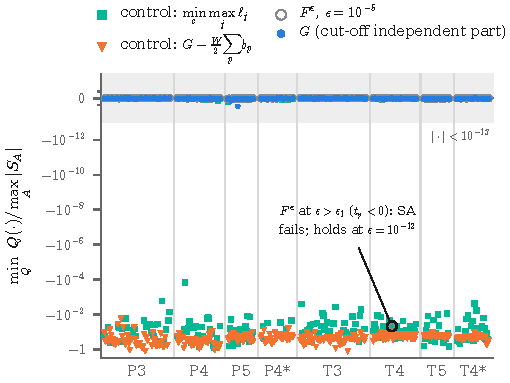
\includegraphics[width=0.6\textwidth]{fig/fig3_numerics.pdf}
\caption{Smallest facet value $\min_QQ(\cdot)/\max_A|S_A|$ of $\mathcal{C}_3,\mathcal{C}_4,\mathcal{C}_5$
(7, 20 and 372 facets) for 308 random configurations on pairs of pants (P) and one-holed tori (T) with two
metrics of common marking, $N=3,4,5$ parties (asterisk: wider parameter ranges). $G$ and $F^\eps$ lie at
rounding level; the single $F^\eps$ outlier has $\eps>\eps_1$ and is removed at smaller $\eps$, as
Theorem~2(i) of the Letter (Theorem~\ref{thm:HRTcone}(ii)) predicts. Two control functionals violate facets in most configurations.}
\label{fig:numericsSM}
\end{figure}

\emph{Results} (Table~\ref{tab:schottky} and Fig.~\ref{fig:numericsSM}). Over 308 configurations and 4428 regions, $G$ satisfies every facet
to rounding and is $\eps$-independent to $2\times10^{-14}$ between $\eps=10^{-3}$ and $10^{-5}$. The single violation by $F^\eps$ is the
threshold effect predicted by Theorem~\ref{thm:graph}: in that configuration a marked point is very close to its neighbour, $d_p$ is
large and $\min_pt_p(10^{-5})=-1.73<0$, i.e.\ $\eps>\eps_1$; the violated facet is subadditivity, which is unbalanced. At
$\eps=10^{-12}$ all facets hold (smallest value $-8\times10^{-17}$). Both controls violate facets in most configurations.
\emph{Limitations:} bounded word length (evidence, not proof, that the true minimiser was found); on the tori no minimiser used a
closed geodesic; the explicit cell graph of Theorem~\ref{thm:graph} was built only on the disc; these tests check the conclusion
$G\in\CN$.

\subsection{Identities}

\emph{Disc, exact graph realisation} (\texttt{disc\_exact.py}, seed 7). $X=\Hyp$, $k\in\{1,2,3\}$ metrics realised as configurations of
the same cyclically ordered marked points (pure $\AdS$ is $k=2$, $w=\frac12$), random horoball normalisations, random party
assignments with $N+2$ to $N+4$ pieces. $G$ is computed three ways: as $F^\eps-\sum_pt_pb_p$; as $\min_c\sum_\tau\mu'(\tau)i(\tau,c)$ with
$\mu'(\tau)$ the Liouville masses (logarithms of cross-ratios) of pairs of non-adjacent pieces; and as the min-cut of the explicit cell
graph of Theorem~\ref{thm:graph} (arrangement in the Klein model, one generic chord per class). For $N=3,4,5$ (300, 200, 60 trials)
the three agree to $5.3\times10^{-14}$, and all facets hold for $F^\eps$ and for $G$ (smallest relative values $-10^{-15}$ and
$-1.5\times10^{-14}$). $G$ satisfies the unbalanced facets too, a non-trivial check since it has no divergent terms.

\emph{Cylinder, renormalised Crofton formula} (\texttt{cylinder\_identity.py}). $\Hyp/\langle z\mapsto e^\ell z\rangle$, 2--5 marked points on
one boundary, random normalisations; for single arcs winding $0,1,2$ times, $i(\mbar',c)$ is computed as an explicit sum over test
classes truncated at 40 periods (largest truncated mass $<10^{-16}$). In 181 cases
$\max|\ell^\eps(c)-i(\mbar',c)-\sum_pe_p\log(1/\eps d_p)|=5.7\times10^{-14}$; for the core geodesic
$\sum_\tau\mbar(\tau)i(\tau,\mathrm{core})=\ell$ to $4\times10^{-16}$.

\emph{Facet lists and contraction maps} (\texttt{cones.py}, \texttt{check\_facets.py}, \texttt{contraction\_mrv.py}). The facet lists
reproduce the orbit sizes of Ref.~\cite{AvisHernandezCuenca2023} (for $\mathcal C_5$: 15, 20, 45, 72, 90, 10, 60, 60, total 372). Two
independent searches find a weighted contraction map for every orbit representative except one $\mathcal C_5$ orbit, consistent with
Refs.~\cite{AvisHernandezCuenca2023,GHHS2026}; 200 random graph models per $N$ satisfy all facets; the non-holographic vector of
Ref.~\cite{Bao2015} violates them.

\subsection{Earlier tests of the contraction-map inequalities and of the slice geometry}

\begin{table}[h]
\caption{Further tests (violations/trials). The scripts are \texttt{contraction.py}, \texttt{annulus\_test.py 1 3000 25.0},
\texttt{fourholed\_test.py 3 600 7 fn}, \texttt{fourholed\_certified.py 3 40}, \texttt{lemmaA\_test.py 0 400},
\texttt{separation\_check.py 0}, \texttt{pleated\_btz\_check.py}, \texttt{spacelike\_check.py}.}
\label{tab:earlier}
\begin{ruledtabular}
\begin{tabular}{p{0.34\textwidth}p{0.30\textwidth}p{0.28\textwidth}}
test & result & control\\
\hline
Contraction-map certificates (SSA, MMI, 5- and 7-party cyclic), exhaustive search and integer verification & maps found and verified & reversed MMI: no map\\
Cylinder ($\pi_1=\Z$), interval parties, $k=1,2,3$ metrics, same class in all; SSA, MMI, 5-party cyclic (3000 each), 7-party (750) & $0$ violations; smallest slack $-2\times10^{-13}$ & $\min_c\max_j\ell_j$: 923/3000 (MMI), 559/3000 (5-cyclic)\\
Four-holed sphere ($\pi_1=F_3$), whole boundaries, Fenchel--Nielsen metrics, $k=1,2,3$; MMI, SSA & $0/600$ each; essential curve in a minimal cut in $\ge99\%$ & $\max$ functional: 299/600\\
Same, certified enumeration (ping-pong Schottky groups, branch and bound over all words), $k=1,2$ & $0/40$ each & ---\\
Lemma~\ref{lem:A} itself on the cylinder, exact integers, arbitrary input cuts & dominating output found in 7800/7800 & reversed MMI: none in 1077/2400\\
Separation Lemma, random acausal circles & $0/160{,}000$; smallest ratio $1.00005$ & crossing triangles: timelike pairs in $16\%$\\
Pleated slice of rotating BTZ, fans spiralling into the horizon, $\ell_L\ne\ell_R$ & $0/360{,}000$ pairs & triangle across the horizon: 113/90,000\\
Lightlike tilt of pleats (Remark~\ref{rem:tilt}) & normalised $\det$ of face normals constant for $\ell_L=\ell_R$, decays to $0$ otherwise & ---\\
\end{tabular}
\end{ruledtabular}
\end{table}

These earlier tests (Table~\ref{tab:earlier}) predate the full-cone results and check the contraction-map inequalities, Lemma~\ref{lem:A}
on the cylinder, and the acausality of pleated slices. Three earlier test versions were found to be vacuous (an essential curve
rarely entered a minimal cut) or to use a non-discrete representation; they are not counted. Lemma~\ref{lem:A} has been tested
directly only for $\pi_1=\Z$, and the embedding part of Proposition~\ref{prop:P} is not tested numerically.

\subsection{Matter in $2+1$ dimensions: Vaidya tests}\label{sec:numvaidya3}

These tests concern Secs.~\ref{sec:nu}--\ref{sec:jacobi}. They test the crossing inequality, Lemma~\ref{lem:N3} and
Proposition~\ref{prop:J}; they cannot test (JM) itself or Theorem~\ref{thm:Hprime}, which would need an independent HRT
solver with homology on all slices.

\begin{sloppypar}
\emph{Thin-shell Vaidya--BTZ, two-sided, $\pi_1=\Z$} (\texttt{vaidya\_btz\_first\_order.py 0}, 23\,s; \texttt{vaidya\_btz\_exact.py},
77\,s). Eternal BTZ ($M_1=1$) with a null shell from the right boundary at boundary time $v_0$, mass $M_2=1+\Delta M$ after it;
metric $-(r^2-M(v))dv^2+2dvdr+r^2d\phi^2$, NEC $\Leftrightarrow\Delta M\ge0$; $L(h)=2\pi$. \emph{First order}, $D=D_0+\Delta M\,D_1$ with
$D_1=\frac12\int\theta(v-v_0)(dv/ds)^2ds$ along vacuum geodesics, on a wiggly boundary slice ($t_R=0.6+0.4\sin(\phi+0.3)$,
$t_L=0.4+0.3\sin(2\phi+1.1)$) and 400 random quadruples on the lifted circle: the vacuum rectangle values $B_0$ are positive in all, and
$\max(-B_1/B_0)=0.0073$ (a first-order NEC violation would need $\Delta M>137$). Lemma~\ref{lem:N3}: $d^{(0)}_n-2\pi=-2.4$,
$-1.3\times10^{-2}$, $-2.5\times10^{-5},\dots$, and $d^{(1)}_n=2.0\times10^{-3},3.6\times10^{-5},\dots,2\times10^{-16}$: $d_n$ increases to
$L(h)$ with vanishing first-order shift of the limit, as predicted. \emph{Exact} single-crossing geodesics (a BTZ($M_2$) piece and a
BTZ($M_1$) piece joined at the critical break point on the shell, equivalent to the refraction law) reproduce $D_0$ to
$4\times10^{-16}$ at $\Delta M=0$ and $dD/d\Delta M=0.059838$ from both codes. For $(t_R,t_L)\in\{(0.6,0.2),(3,0),(3,2),(1,3)\}$ and
$\Delta M$ from $+3$ to $-0.97$, between 51 and 120 random rectangles per case, no rectangle has $\nu<0$, and $d_n\to2\pi$ throughout. For
strongly NEC-violating shells the positivity margin collapses ($\min\nu/\nu_0\to0.03$) at the edge of the solvable region but does not
become negative there; configurations whose geodesics re-enter the shell region (e.g.\ $t_R=3,t_L=2$, $|\Delta\phi|\lesssim1.5$) are
outside the single-crossing solver and excluded. This solver therefore does not exhibit the necessity of the NEC.
\end{sloppypar}

\begin{sloppypar}
\emph{Smooth planar Vaidya--$\AdS$, test of Proposition~\ref{prop:J}} (\texttt{check\_nec\_sign.py}, \texttt{check\_jacobi\_identities.py},
\texttt{jacobi\_sign\_vaidya.py}, 5\,min; \texttt{nearnull\_slice.py}, 25\,s). $ds^2=z^{-2}(-(1-m(v)z^2)dv^2-2dv\,dz+dx^2)$ with
$m=m_0+\Delta m\,(1+\tanh((v-v_0)/w))/2$; NEC $\Leftrightarrow m'\ge0$ ($R_{ab}+2g_{ab}=\frac12zm'\delta^v_a\delta^v_b$, checked symbolically).
Geodesics by Hamiltonian shooting (DOP853, rtol $10^{-12}$, cutoff $2\times10^{-4}$, mass continuation); mixed derivatives by 4-point
differences with $h=0.02$ (step check $h=0.04,0.02,0.01$: $D_{ll}=-0.24989,-0.24860,-0.24828$). With $+$ the future-right and $-$ the
future-left null direction and $x_1<x_2$, $D_{++}=D_{lk}$, $D_{--}=D_{kl}$, $D_{+-}=D_{ll}$, $D_{-+}=D_{kk}$. Endpoint pairs
$(v,x)$: $((0,0),(0.4,1.5))$, $((-0.3,0),(0.6,1.2))$, $((0.5,0),(-0.2,1.3))$, $((0.2,0),(0.2,2.0))$. Results in
Table~\ref{tab:jacobi}: all 16 NEC sign predictions hold, the vacuum cross terms vanish to solver accuracy, and \emph{every}
NEC-violating case flips the sign of both cross terms. On a spacelike boundary slice that is nearly null at the endpoints (slope
$+S$ at $P=(0,0)$, $-S$ at $Q=(0.4,1.5)$), the crossing density $\partial_s\partial_tD$ is, for $S=0.9$ and $S=0.99$: vacuum $+0.182$, $+0.019$;
NEC shell $\Delta m=+1.5$: $+0.400$, $+0.265$; NEC-violating $\Delta m=-0.8$: $+0.061$, $\mathbf{-0.117}$. Without the NEC the crossing
inequality, here ordinary SSA for intervals of one boundary slice, fails on an admissible slice, consistent with
Ref.~\cite{CallanHeHeadrick2012}.
\end{sloppypar}

\begin{table}[h]
\caption{Signs of the null mixed derivatives of $D$ in smooth planar Vaidya--$\AdS$ (four endpoint configurations per row;
ranges over the configurations). Proposition~\ref{prop:J} predicts $D_{lk},D_{kl}>0$ and $D_{ll},D_{kk}\le0$ under the NEC, with
$D_{ll}=D_{kk}=0$ in vacuum. Last column: crossing density on a spacelike boundary slice with endpoint slopes $\pm0.5/\mp0.3$.}
\label{tab:jacobi}
\begin{ruledtabular}
\begin{tabular}{lccccc}
geometry $(m_0,\Delta m,v_0,w)$ & $D_{lk}$ & $D_{kl}$ & $D_{ll}$ & $D_{kk}$ & $\nu$-density\\
\hline
vacuum $(1,0,0,0.3)$ & $0.64\dots10.9$ & $0.72\dots45.8$ & $\le6\times10^{-7}$ & $\le6\times10^{-7}$ & $>0$\\
NEC $(1,1.5,0,0.3)$ & $>0$ & $>0$ & $-0.11\dots-0.40$ & $-0.005\dots-0.06$ & $>0$\\
NEC $(0.5,4,0.2,0.25)$ & $>0$ & $>0$ & $-0.06\dots-0.45$ & $-0.008\dots-0.22$ & $>0$\\
NEC-violating $(1,-0.8,0,0.3)$ & $>0$ & $>0$ & $+0.06\dots+0.23$ & $+0.003\dots+0.04$ & $>0$\\
NEC-violating $(1,-0.95,0.2,0.25)$ & $>0$ & $>0$ & $+0.013\dots+0.11$ & $+0.001\dots+0.06$ & $>0$\\
\end{tabular}
\end{ruledtabular}
\end{table}

\emph{Wheeler--DeWitt patch} (\texttt{wdw\_singularity.py}): the numbers quoted in Sec.~\ref{sec:JMsuff}.

\subsection{Strips in $\mathrm{AdS}_4$: thin-shell Vaidya}\label{sec:numstrips}

\begin{sloppypar}
These tests concern Sec.~\ref{sec:strips} (\texttt{vaidya\_strips.py}, about 8\,s before plotting;
\texttt{verify\_finite\_graph.py}; \texttt{check\_kk\_ricci.py}; \texttt{expand\_facets.py}). Geometry
$ds^2=z^{-2}[-(1-\Theta(v)z^3)dv^2-2dv\,dz+dx^2+dy^2]$, AdS radius and final horizon radius one; the strip area functional
$\mathcal A=\int dx\,z^{-2}\sqrt{1-fv'^2-2v'z'}$ with the equations of Liu and Suh~\cite{LiuSuh2014} (Sec.~III.A). For each shell ratio
$r=z_c/z_t$ a scalar equation fixes the turning point from the width; all intersections visible in the parameterised scan are
bracketed and refined, and up to three candidates (two shell-crossing, one static) are compared, with the smallest area selected; the
family is not assumed monotone in boundary time. An analytic short-strip bound excludes deep radially returning branches in this
reflection-symmetric family (for the largest width, $z_t\le0.748$ and all returning solutions lie outside the final horizon). The
reflection-symmetric solver is a numerical restriction separate from the transverse-translation theorem; the matching formula
\eqref{eq:T7} is an analytic input, and the computation does not independently establish symmetry or common maximin slices.
\end{sloppypar}

Configurations: contiguous strips of widths $(0.10,0.14,0.18,0.16,0.12)$, and separated width-$0.12$ strips with gap $0.0741$; the
first 3, 4 and all 5 parties of each (six cases). All 372 five-party facets~\cite{HernandezCuenca2019} (eight orbits under $S_6$,
expanded from the author-maintained representatives; absent parties set empty) are evaluated at 551 boundary times (a uniform
401-point grid on $[-0.025,0.7724]$, the quench and static-admissibility times, and refinements in the narrow saturation windows):
$1\,229\,832$ evaluations. The cone test uses a common radial truncation $\eps=10^{-4}$, $\mathcal A_\eps=2/\eps+a_\eps$; for a union with
$m_I$ connected intervals every matching has divergence $2m_I/\eps$, and $\sum_Ic_I\mathcal A_\eps(I)=(2/\eps)\sum_Ic_Im_I+\sum_Ic_Ia_\eps(I)$ is
evaluated with the integer UV coefficient kept exactly (it is nonnegative in every case). The minimum margin is $-7.11\times10^{-14}$, with
none below the tolerance $-2\times10^{-8}$; the separated pair loses mutual information at $t/z_h\simeq0.2336006115$
(Figs.~\ref{fig:strips1}, \ref{fig:strips2}). Validation: width and time residuals $1.2\times10^{-14}$ and $6\times10^{-16}$; quadrature
refinement (160 to 320 nodes) changes width, time and finite area below $9\times10^{-15}$; 48 independent multistart solves agree with
continuation to $1.6\times10^{-12}$. These are sampled floating-point checks at a literal radial truncation, which is a different regulator
from the endpoint prescription of Theorem~\ref{thm:strips}; they are evidence, not an all-time proof. The exact-rational graph check
verifies 756 min-cut/matching equalities (3--8 endpoints), and the Kaluza--Klein Ricci identity \eqref{eq:T4} is checked symbolically.

\begin{figure}[h]
\centering
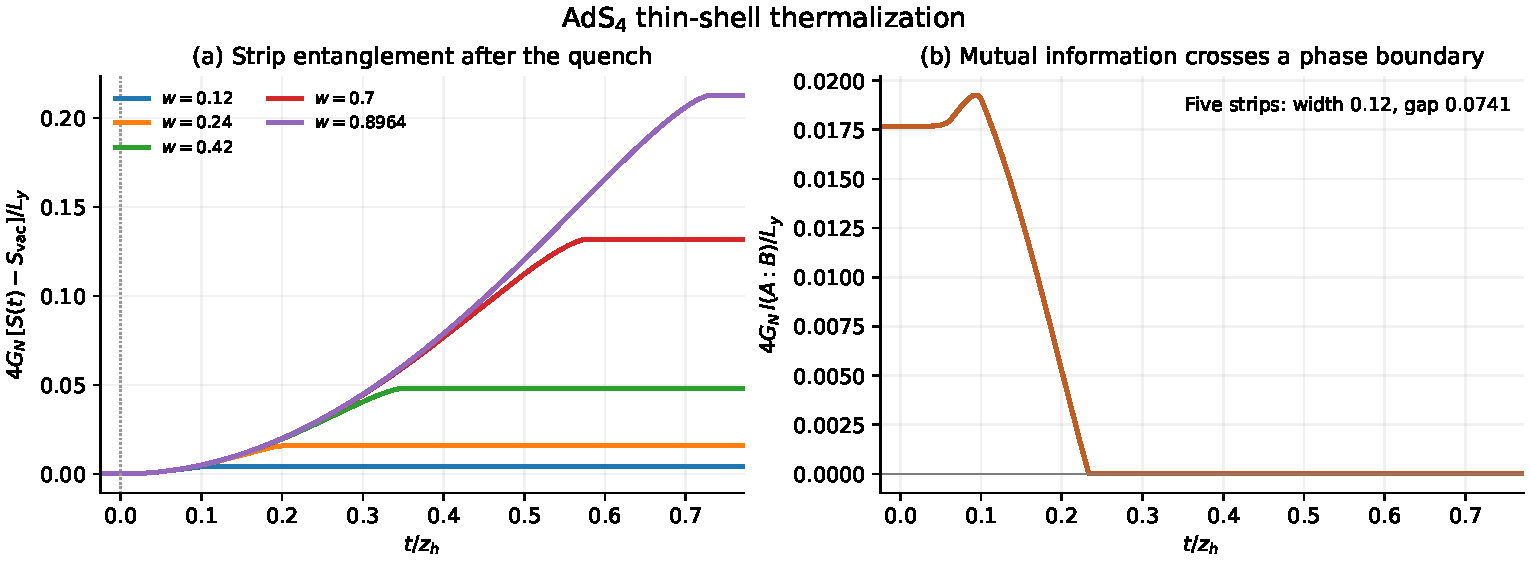
\includegraphics[width=\textwidth]{fig/strips_vaidya_entropy_cone.pdf}
\caption{Thin-shell thermalisation in $\mathrm{AdS}_4$. (a)~Vacuum-subtracted strip entropies, in units $4G_NS/L_y$, for several widths
(final horizon radius one). (b)~Mutual information between neighbouring width-$0.12$ strips separated by $0.0741$; the connected phase
disappears at $t\simeq0.23360$. At 551 sampled times all 372 five-party facets hold for the contiguous and separated three-, four- and
five-strip configurations, with largest negative residual $7.11\times10^{-14}$ (roundoff).}
\label{fig:strips1}
\end{figure}

\begin{figure}[h]
\centering
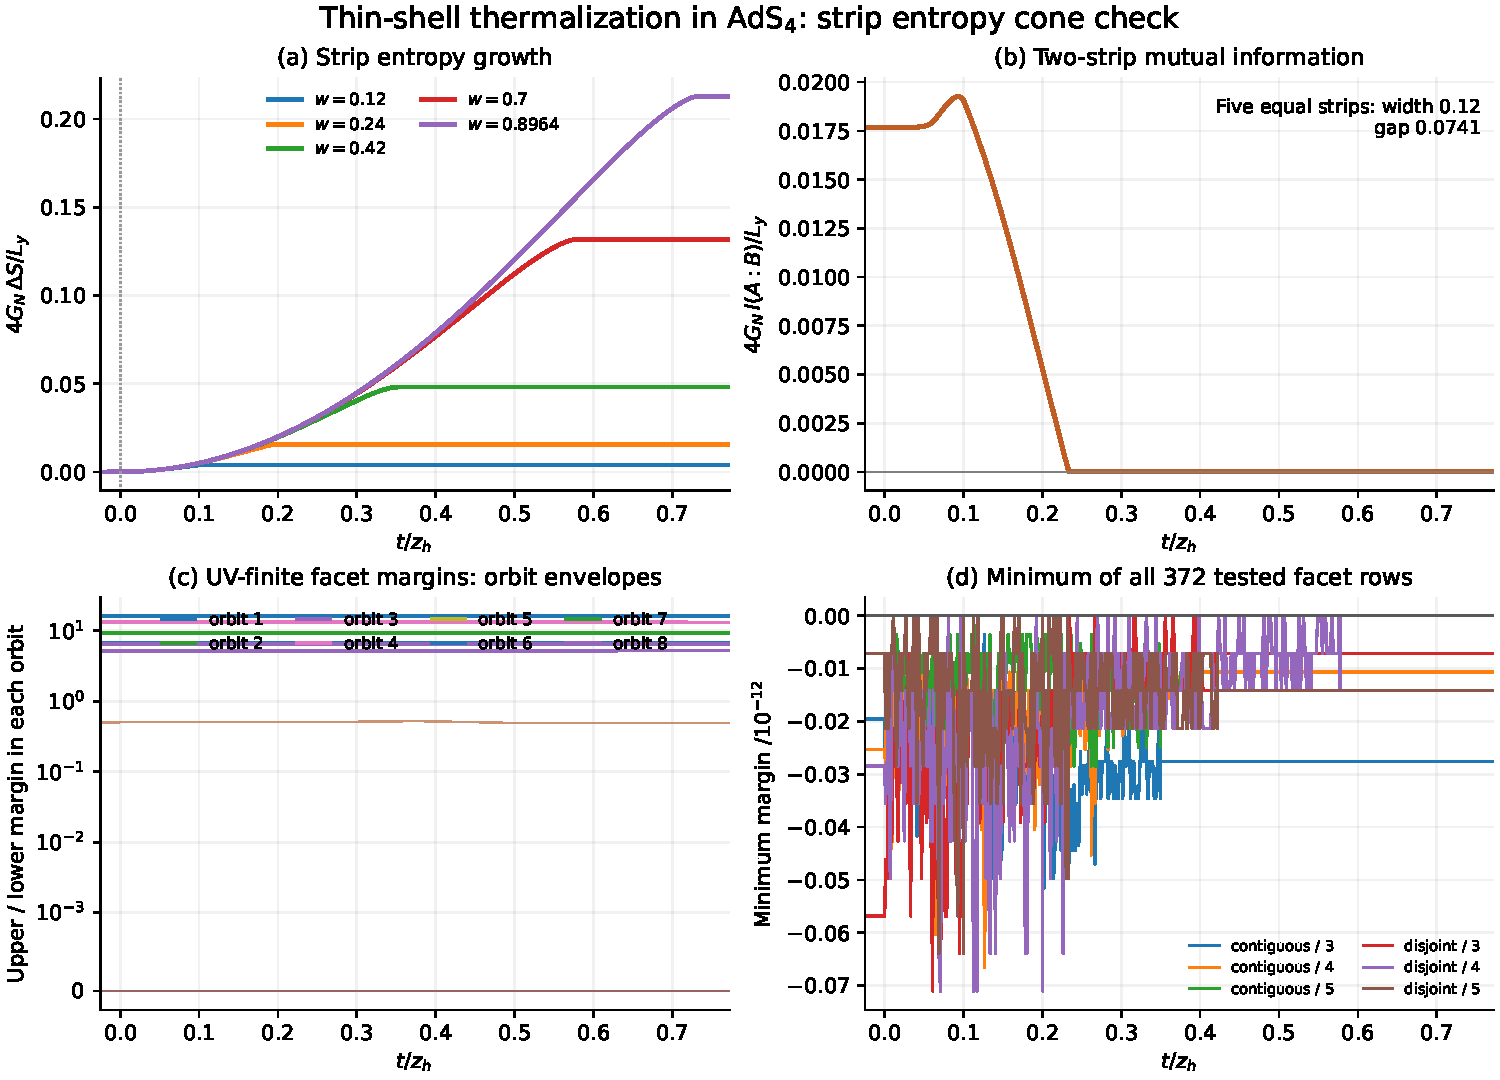
\includegraphics[width=0.8\textwidth]{fig/strips_vaidya_diagnostics.pdf}
\caption{Diagnostics for Fig.~\ref{fig:strips1}. (a),~(b) as there. (c)~Upper and lower envelopes of the UV-finite facet margins in
each of the eight facet orbits. (d)~Minimum over all 372 facets, in units of $10^{-12}$, for the six configurations (contiguous and
disjoint, 3, 4, 5 parties): all minima are at roundoff level and are shown with their signs.}
\label{fig:strips2}
\end{figure}

% ===================================================================================================
\section{Status of statements and cited inputs}\label{sec:status}

\begin{table}[h]
\caption{Status of the unconditional statements (Secs.~\ref{sec:setting}--\ref{sec:main}). ``Proved'' means a complete argument is given here, using only the cited inputs listed below
the table.}
\label{tab:status}
\begin{ruledtabular}
\begin{tabular}{p{0.45\textwidth}p{0.5\textwidth}}
statement & status\\
\hline
Lemma~\ref{lem:A} (topological contraction) & proved\\
Proposition~\ref{prop:crofton} (renormalised Crofton), Corollary~\ref{cor:decomp} (decomposition) & proved; checked numerically to $6\times10^{-14}$\\
Theorem~\ref{thm:graph} (graph realisation), Corollaries~\ref{cor:cone}, \ref{cor:contraction} & proved; graph checked on the disc to $5\times10^{-14}$\\
Proposition~\ref{prop:length} (length formula) & proved\\
Theorems~\ref{thm:C}, \ref{thm:E} (slices $=$ acausal Cauchy slices of $\Mbar$) & proved for $\Gamma\ne1$, given the cited action on $\EG$\\
Lemmas~\ref{lem:sep}, \ref{lem:tri}; Proposition~\ref{prop:P} & proved; not new in substance~\cite{MazzoliViaggi2022}\\
Lemma~\ref{lem:T} (spun family) & proved, given the existence of triangulations with prescribed vertices~\cite{Hatcher1991}\\
Theorem~\ref{thm:H} & proved, for slices satisfying (S1)--(S3), i.e.\ acausal Cauchy slices of $\Mbar$\\
Proposition~\ref{prop:Splus}, Corollary~\ref{cor:smoothH} (smooth uniformly spacelike slices) & proved, given Bernal--S\'anchez Theorem~1.1 and Remark~4.14~\cite{BernalSanchez2006} and Geroch's theorem\\
Theorem~\ref{thm:HRTcone} (HRT vector in $\CN$, every valid inequality) & proved, given the above\\
Theorem~\ref{thm:equality} (cone equality) & proved, given Bao \emph{et al.}~\cite{Bao2015}, Sec.~3.1, Lemma~4 and the graph characterisation of $\CN$\\
Matter without (JM); higher dimensions beyond invariant strips; extremal horizons; conical defects; non-orientable quotients; achronal slices with null pieces; homology regions not on a Cauchy slice; quantum corrections & not covered\\
\end{tabular}
\end{ruledtabular}
\end{table}

\begin{table}[h]
\caption{Status of the conditional results (Secs.~\ref{sec:matter}--\ref{sec:strips}). ``Proved mod X'' means a complete argument is
given here, assuming X and the cited inputs listed below.}
\label{tab:status2}
\begin{ruledtabular}
\begin{tabular}{p{0.45\textwidth}p{0.5\textwidth}}
statement & status\\
\hline
\multicolumn{2}{l}{\emph{Matter in $2+1$ dimensions (Secs.~\ref{sec:matter}--\ref{sec:jacobi}); (R) is assumed throughout}}\\
Proposition~\ref{prop:JMvac} ((JM) in vacuum) & proved, given Lemma~\ref{lem:P}\\
Proposition~\ref{prop:JMcons} (consequences of (JM)) & proved mod (JM); uses Epstein's theorem~\cite{Epstein1966}\\
Remark~\ref{rem:false} (joint maximin for linking pairs; single-class maximin for non-simple classes) & false as stated; not used\\
Lemma~\ref{lem:P} (componentwise null projection) & proved mod Wall's projection lemma~\cite{Wall2014} and (R1), (R4)\\
Lemma~\ref{lem:Q}, Proposition~\ref{prop:sandwich} (sandwich) & proved (no maximin hypothesis)\\
Theorem~\ref{thm:Hprime} (Theorem H$'$) & proved mod (JM)\\
Lemmas~\ref{lem:S}, \ref{lem:X} (crossing inequality), \ref{lem:Ccont}, \ref{lem:N3}, \ref{lem:N4}, \ref{lem:N2}; Corollary~\ref{cor:I} & proved mod (JM), (R); uses residual finiteness, Hall's and Scott's theorems~\cite{Hall1949,Scott1978}\\
Theorem~\ref{thm:M} (Theorem~4 of the Letter) & proved mod (JM), (R); not unconditional\\
Proposition~\ref{prop:bellmatter} (Bell-pair decomposition, all valid inequalities for intervals) & proved mod (JM), (R)\\
Propositions~\ref{prop:U}, \ref{prop:E} (usc; existence of maximisers; continuity of $D$) & proved mod (K), Ioffe's theorem~\cite{Ioffe1977}, Fefferman--Graham asymptotics\\
Proposition~\ref{prop:W2} ((JM) from (K) and (Reg)) & proved mod (K), (Reg), Sion's theorem~\cite{Sion1958}\\
(K) for NEC thin-shell Vaidya--BTZ wormholes & fails (ODE comparison; numerics)\\
Proposition~\ref{prop:J} (local crossing positivity) & proved mod (ND), Fefferman--Graham falloff; no maximin hypothesis\\
NEC necessity (Table~\ref{tab:jacobi}) & numerical: crossing density $-0.117$ on an admissible slice for a NEC-violating shell\\
\multicolumn{2}{l}{\emph{Strips in $d+1\ge4$ dimensions (Sec.~\ref{sec:strips})}}\\
Area identity \eqref{eq:T3}, Proposition~\ref{prop:KKric} (effective NEC) & proved; checked symbolically\\
Lemmas~\ref{lem:BV}, \ref{lem:liftext}, \ref{lem:relcut} (symmetry by averaging; extremal lifts; relative cutoff) & proved\\
Theorem~\ref{thm:stripsym} (invariant HRT surface) & proved mod (H4) (stable reduced maximin; boundary behaviour~\cite{Sorce2019})\\
Lemmas~\ref{lem:stripcompact}, \ref{lem:regmax} & proved under their stated compact-slab and regularity hypotheses\\
Matching formula \eqref{eq:T7} & proved mod (H3), (H4) (laminar joint maximin)\\
Theorem~\ref{thm:finitegraph} (finite graph theorem) & proved; 756 exact checks\\
Theorem~\ref{thm:strips} (Theorem~5 of the Letter) & proved mod (H1)--(H4); not a statement about all NEC spacetimes\\
\end{tabular}
\end{ruledtabular}
\end{table}

\emph{Cited inputs.} (i) Structure of the spacetimes: proper discontinuity of $\Gamma$ on $\Dt$ and on $\EG$ including the boundary,
and the identification of the asymptotic regions~\cite{Mess2007,Barbot2008,BKS2011}. (ii) Convex cocompactness and measure zero of
limit sets of Schottky-type Fuchsian groups. (iii) The Crofton formula~\cite{Santalo1976}. (iv) Geodesic representatives and minimal
position~\cite{Epstein1966,FarbMargalit2012}. (v) Triangulations of compact surfaces with prescribed vertices~\cite{Hatcher1991}.
(vi) Smooth Cauchy extension~\cite{BernalSanchez2006} and the Cauchy-surface criterion for global hyperbolicity~\cite{Geroch1970}.
(vii) For the cone statements: graph models, their closedness and polyhedrality, and the realisation of graphs by hyperbolic
surfaces~\cite{Bao2015}. No completeness statement about contraction maps~\cite{BaoFuruyaNaskar2025} and no characterisation theorem
for currents~\cite{MartinezGranadoThurston2026} is used. (viii) For the matter results: Wall's null projection and maximin
framework~\cite{Wall2014,MarolfWallWang2019}; the area theorem for achronal null boundaries~\cite{CDGH2001}; Epstein's
theorem~\cite{Epstein1966}; residual finiteness of free groups, subgroup separability~\cite{Hall1949} and Scott's
theorem~\cite{Scott1978}; Ioffe's semicontinuity theorem~\cite{Ioffe1977}; Sion's minimax theorem~\cite{Sion1958}; the
structure of globally hyperbolic spacetimes with timelike boundary~\cite{AkeFloresSanchez2021}; topological
censorship~\cite{GSWW1999}. Existence and regularity of (homotopy-restricted) maximin slices are \emph{assumed}, through (JM).
(ix) For the strips: Wall's Theorems~15, 17, Corollary~17(h) and Theorem~11~\cite{Wall2014}; same-anchor extremal
asymptotics~\cite{Sorce2019}; the graph characterisation of $\CN$~\cite{Bao2015}; existence and regularity of stable reduced
maximin are \emph{assumed}, through (H4).

\emph{Standing assumptions (Secs.~\ref{sec:setting}--\ref{sec:main}).} Orientable surfaces with funnel ends only; the same marking on both chiral surfaces; positive weights
(positivity is essential: the $\max$ functional violates the inequalities); the same class in all metrics; regions are unions of
elementary pieces on one boundary Cauchy slice; the HRT entropy is the leading classical term defined in
Definition~\ref{def:HRT}.

\bibliographystyle{apsrev4-2}
\bibliography{refs}

\end{document}
